\documentclass[a4paper, 12pt]{report}

\usepackage[dvipsnames]{xcolor}

%%%%%%%%%%%%%%%%
% Set Variables %
%%%%%%%%%%%%%%%%

\def\useItalian{0}  % 1 = Italian, 0 = English

\def\courseName{Advanced Algorithms}

\def\coursePrerequisites{Sufficient knowledge of computability theory, algorithm complexity, number theory and probability}

\def\book{\curlyquotes{Algorithm Design},\\ J. Kleinberg, É. Tardos}

\def\authorName{Simone Bianco}
\def\email{bianco.simone@outlook.it}
\def\github{https://github.com/Exyss/university-notes}
\def\linkedin{https://www.linkedin.com/in/simone-bianco}

% \def\authorName{Alessio Bandiera}
% \def\email{alessio.bandiera02@gmail.com}
% \def\github{https://github.com/aflaag-notes}
% \def\linkedin{https://www.linkedin.com/in/alessio-bandiera-a53767223}

%%%%%%%%%%%%
% Packages %
%%%%%%%%%%%%

\usepackage{../../packages/Nyx/nyx-packages}
\usepackage{../../packages/Nyx/nyx-styles}
\usepackage{../../packages/Nyx/nyx-frames}
\usepackage{../../packages/Nyx/nyx-macros}
\usepackage{../../packages/Nyx/nyx-title}
\usepackage{../../packages/Nyx/nyx-intro}

%%%%%%%%%%%%%%
% Title-page %
%%%%%%%%%%%%%%

\logo{../../packages/Nyx/logo.png}

\if\useItalian1
    \institute{\curlyquotes{\hspace{0.25mm}Sapienza} Università di Roma}
    \faculty{Ingegneria dell'Informazione,\\Informatica e Statistica}
    \department{Dipartimento di Informatica}
    \ifdefined\book
        \subtitle{Appunti integrati con il libro \book}
    \fi
    \author{\textit{Autore}\\\authorName}
\else
    \institute{\curlyquotes{\hspace{0.25mm}Sapienza} University of Rome}
    \faculty{Faculty of Information Engineering,\\Informatics and Statistics}
    \department{Department of Computer Science}
    \ifdefined\book
        \subtitle{Lecture notes integrated with the book \book}
    \fi
    \author{\textit{Author}\\\authorName}
\fi


\title{\courseName}
\date{\today}

% \supervisor{Linus \textsc{Torvalds}}
% \context{Well, I was bored\ldots}

%%%%%%%%%%%%
% Document %
%%%%%%%%%%%%

\addbibresource{./references.bib}

\begin{document}
    \maketitle

    % The following style changes are valid only inside this scope 
    {
        \hypersetup{allcolors=black}
        \fancypagestyle{plain}{%
        \fancyhead{}        % clear all header fields
        \fancyfoot{}        % clear all header fields
        \fancyfoot[C]{\thepage}
        \renewcommand{\headrulewidth}{0pt}
        \renewcommand{\footrulewidth}{0pt}}

        \romantableofcontents
    }

    \introduction

    %%%%%%%%%%%%%%%%%%%%%

    \chapter{Approximation algorithms}

    \section{Coping with untractability}

    In computer science and optimization, approximation algorithms are algorithms designed to find near-optimal solutions to computational problems that are $\mathsf{NP}$-hard, i.e. every problem that is verifiable in polynomial time can be reduced to them. Even though the $\mathsf{P} \stackrel{?}{=} \mathsf{NP}$ question is still unsolved -- which corresponds to determining if every problem efficiently verifiable is also efficiently solvable -- lots of theoretical results make us believe that $\mathsf{P} \neq \mathsf{NP}$. Hence, we usually assume that the conjecture has actually been proven as false. This means that every $\mathsf{NP}$-hard problem is \textbf{untractable}, meaning that there is no polynomial-time algorithm that can solve them exactly in all cases. Hence, \textbf{approximation algorithms} are used to find solutions that are \curlyquotes{good enough} or \curlyquotes{close enough} to the optimal, with a known error bound, sacrificing exactness for efficiency.

    In particular, approximation algorithms are used for \textbf{optimization problems}, i.e. every type of problem that asks to find a structure that maximizes or minimizes a property. An approximation algorithm is typically evaluated based on how close its solution is to the optimal solution. The approximation ratio is defined as the worst-case ratio between the cost of the solution produced by the algorithm and the cost of the optimal solution.
    
    For instance, if an algorithm for a minimization problem has an approximation ratio of $\rho$, then the value $\ell$ of the approximate solution is guaranteed to be at most $\rho$ times as large as the optimal solution value $\ell^*$.
    \[\ell \leq \rho \ell^* \implies \rho = \frac{\ell}{\ell^*}\]
    
    For a maximization problem, instead, the solution is guaranteed to be at least $\rho$ times as large as the optimal solution value $\ell^*$.
    \[\ell \geq \rho \ell^* \implies \rho = \frac{\ell^*}{\ell}\]

    \section{Approximations through randomness}

    \label{max_cut}

    The \textbf{Maximum Cut} problem is a fundamental optimization problem in graph theory and combinatorial optimization. In particular, the problem has numerous practical applications, including in network design, statistical physics (particularly in the study of spin glasses), and in various areas of machine learning, where it is used to model problems such as clustering and data partitioning. Given an undirected graph, the goal of the Max-cut problem is to \textbf{partition} the graph's vertices into two disjoint subsets such that the number of edges between the two subsets, i.e. outgoing from one subset to the other, is maximized. This partition is referred to as a \textbf{cut}, while the set of edges whose endpoints don't lie in the same subset is called \textbf{cut-set}. 
    
    \begin{figure}[H]
        \centering

        \begin{tikzpicture}[-,>=stealth,shorten >=1pt,auto,node distance=2cm, thick,main node/.style={scale=0.9,circle,draw,font=\sffamily\normalsize}]

            \node[] (x) []{};
            \node[main node] (1)[fill = Carmine, above left of = x] {};
            \node[main node] (2)[fill = BlueLagoon, above right of = x] {};
            \node[main node] (3)[fill = Carmine, right of = x] {};
            \node[main node] (4)[fill = Carmine, below right of = x] {};
            \node[main node] (5)[fill = BlueLagoon, below left of = x] {};
            \node[main node] (6)[fill = Carmine, left of = x] {};

            \path[every node/.style={font=\sffamily\small}]
                (1) edge[color = Green, line width = 2] (2)
                (2) edge[color = Green, line width = 2] (3)
                (3) edge (4)
                (4) edge[color = Green, line width = 2] (5)
                (5) edge[color = Green, line width = 2] (6)
                (6) edge (1)
                (1) edge (4)
                (2) edge[color = Green, line width = 2] (4)
                (3) edge (5)
                (2) edge (5)
                ;
        \end{tikzpicture}
        \caption{The red vertices and the blue vertices form a cut of the graph. The green edges are the edges of the cut-set.}
    \end{figure}
    
    To distinguish between directed and undirected graphs, in the undirected case we'll define the set of edges $E$ of a graph $G = (V,E)$ as $E \subseteq \binom{V}{2} = \{\{u,v\} \mid u,v \in V\}$, while in the directed case we have that $E \subseteq \{(u,v) \mid u,v \in V\}$, where $(u,v)$ represents and edge $u \to v$.

    \begin{frameddefn}{Cut of a graph}
        Given an undirected graph $G$, a cut of $G$ is a bipartition $(S,T)$ of $G$. The cut-set of a cut $(S,T)$ is defined as $\mathrm{cut}(S,T) = \{e \in E(G) \mid \abs{S \cap e} = 1\}$
    \end{frameddefn}

    The $\mathrm{MC}$ problem is concerned with finding the cut that maximizes the number of edges crossing between the two subsets of the cut (or the total weight of the edges in the cut-set in the weighted case). In particular, we'll focus on the unweighted case of this problem. Unlike its minimization counterpart, i.e. the Min-cut problem, the Max-cut problem is notable for being $\mathsf{NP}$-hard by reduction from the Maximum Independent set problem \cite{garey_npcomp}. The Min-cut problem, instead, is known to lie in $\mathsf{P}$ by reduction to the $s$-$t$ Maximum Cut problem, which is equivalent to the maximum network flow problem.
    
    While finding the optimal solution for the Max-cut problem is computationally intractable for large graphs, significant progress has been made in designing algorithms that can find near-optimal solutions efficiently. One such approach is the famous Goemans-Williamson algorithm, which provides a $(0.878\ldots)$-approximation for $\mathrm{MC}$, i.e. a solution that has at least a $(0.878\ldots)$-th of the edges of the optimal solution. using semidefinite programming and randomization. We'll see this algorithm in later sections. It is known that there exists a constant $c < 1$ such that there cannot exist any $c$-approximation algorithm for $\mathrm{MC}$ unless $\mathsf{P} = \mathsf{NP}$ is true \cite{inapprox_maxcut}, which we assume to be false. For $\mathrm{MC}$, this constant is known to be as small as $\frac{83}{84} \approx 0.988$.

    For now, we'll focus on showing that \textbf{randomness} can be used to get a trivial expected $\frac{1}{2}$-approximation of the problem in polynomial time with a sufficiently high probability. This represents the typical case where randomness can be used to get a good enough polynomial time solution with the small trade-off of having a low probability of getting a solution that is below-expectations.
    
    \begin{algorithm}[H]
        \caption{The random-cut algorithm}
        \textbf{Input:} an undirected graph $G$

        \textbf{Output:} a cut $(S, \overline{S})$ of $G$
        \begin{algorithmic}[1]
            \Function{random-cut}{$G$}
                \State $S \gets \varnothing$
                \For{$v \in V(G)$}
                    \State Flip a fair independent coin and set $c_v$ as the outcome
                    \If{$c_v = 1$}
                        \Comment 1 is heads, 0 is tails
                        \State $S \gets S \cup \{v\}$
                    \EndIf
                \EndFor
                \State Return $(S, \overline{S})$
            \EndFunction
        \end{algorithmic}
    \end{algorithm}

    The runtime of this algorithm is clearly $O(n)$ if $S$ is stored using a set data structure. We also notice that the \textsc{random-cut} algorithm actually doesn't even care about the graph structure: we're just flipping coins. This idea can be used for many other problems. We now prove that it yields an expected $\frac{1}{2}$-approximation of $\mathrm{MC}$.

    \begin{framedthm}{}
        Given a graph $G$, let $(S^*, \overline{S^*})$ be an optimal solution to $\mathrm{MC}(G)$. Given the output $(S, \overline{S})$ of $\textsc{random-cut}(G)$, it holds that:
        \[\Exp[\abs{\mathrm{cut}(S, \overline{S})}] \geq \frac{\abs{\mathrm{cut}(S^*, \overline{S^*})}}{2}\]
    \end{framedthm}

    \begin{proof}
        For any edge $e \in E(G)$, we know that $e \in \mathrm{cut}(S, \overline{S})$ if and only if $\abs{S \cap e} = 1$. If $e = \{u,v\}$, this is also also equivalent to saying that $u \in S, v \notin S$ or $u \notin S, v \in S$. We notice that:
        \[\begin{split}
            \Pr[e \in \mathrm{cut}(S, \overline{S})] &= \Pr[(u \in S, v \notin S) \lor (u \notin S, v \in S)] \\
            &= \Pr[u \in S, v \notin S] + \Pr[u \notin S, v \in S] - \Pr[u \in S, v \notin S, u \notin S, v \in S] \\
            &= \frac{1}{4} + \frac{1}{4} + 0
        \end{split}\]

        thus, we get that:
        \[\Exp[\abs{\mathrm{cut}(S, \overline{S})}] = \sum_{e \in E(G)} 1 \cdot \Pr[e \in \mathrm{cut}(S, \overline{S})] = \frac{\abs{E(G)}}{2}\]

        Finally, since each cut-set is by definition a subset of $E(G)$, we know that $\abs{\mathrm{cut}(S^*, \overline{S^*})} \leq E(G)$, concluding that:
        \[\Exp[\abs{\mathrm{cut}(S, \overline{S})}] =  \frac{\abs{E(G)}}{2} \geq \frac{\abs{\mathrm{cut}(S^*, \overline{S^*})}}{2}\]
    \end{proof}

    On first impact, this algorithm may seem useless: the solution is only \textit{expected} to be a $\frac{1}{2}$-approximation of the optimal maximum cut of the input graph. In fact, if we are very unlucky, the solution could contain all the edges or the graph or even no edges at all. However, this algorithm is actually enough. In fact, we can show that, by running this algorithm a sufficient amount of times, the probability of getting a bad solution can be highly reduced. 

    \begin{algorithm}[H]
        \caption{The $t$-times random-cut algorithm}
        \textbf{Input:} an undirected graph $G$ and a non-negative integer $t$

        \textbf{Output:} a cut $(S, \overline{S})$ of $G$
        \begin{algorithmic}[1]
            \Function{$t$-random-cut}{$G,t$}
                \For{$i \in [\ceil{t}]$}
                    \State $(S_i, T_i) \gets \Call{random-cut}{G}$
                \EndFor
                \State Return $(S, \overline{S}) \in \argmax\limits_{i \in [\ceil{t}]} \abs{\mathrm{cut}(S_i, T_i)}$
            \EndFunction
        \end{algorithmic}
    \end{algorithm}

    \begin{framedthm}{}
        Given a graph $G$ and a non-negative integer $t$, let $(S^*, \overline{S^*})$ be an optimal solution to $\mathrm{MC}(G)$. Given the output $(S, \overline{S})$ of $t\textsc{-random-cut}(G)$, it holds that:
        \[\Pr\sbk{\abs{\mathrm{cut}(S, T)} > \frac{(1-\varepsilon)}{2} \abs{\mathrm{cut}(S^*, \overline{S^*})}} > 1-\delta\]

        where $t = \frac{2}{\varepsilon} \ln \frac{1}{\delta}$ and $0 < \varepsilon, \delta < 1$.
    \end{framedthm}

    \begin{proof}
        For each $i \in [\ceil{t}]$, let $C_i = \mathrm{cut}(S_i,T_i)$, where $(S_1, T_1), \ldots, (S_t, T_t)$ are the cuts yielded by the algorithm, and let $N_i = \abs{E(G)} - C_i$. Since $N_i$ is a non-negative random variable, by Markov's inequality we have that:
        \[\Pr[N_i \geq (1+\varepsilon) \Exp[N_i]] \leq \frac{1}{1+\varepsilon} = 1 - \frac{\varepsilon}{1+\varepsilon} \leq 1- \frac{\varepsilon}{2}\]

        Through some algebraic manipulation, and by linearity of the expected value operator, we get that:
        \[\begin{split}
            1- \frac{\varepsilon}{2} &\geq \Pr[N_i \geq (1+\varepsilon) \Exp[N_i]]\\
            &= \Pr[\abs{E(G)}-C_i \geq (1+\varepsilon)(\abs{E(G)} - \Exp[C_i])] \\
            &= \Pr[-\varepsilon \abs{E(G)} \geq C_i - (1+\varepsilon) \Exp[C_i]] \\
        \end{split} \]

        Using the same argument of the previous theorem, we know that $\Exp[C_i] = \frac{\abs{E}}{2}$. Hence, we get that:
        \[\begin{split}
            1 - \frac{\varepsilon}{2} &\geq \Pr[-\varepsilon \abs{E(G)} \geq C_i - (1+\varepsilon) \Exp[C_i]] \\
            &= \Pr[C_i \leq \frac{1-\varepsilon}{2} \abs{E}] \\
            &= \Pr[C_i \leq (1-\varepsilon)\Exp[C_i]]
        \end{split} \]


        We notice that the event of the last probability corresponds to a \curlyquotes{bad solution}, i.e. one whose value is at most $(1-\varepsilon)$-th of the expected value. Since each run of \textsc{random-cut} is independent from the others, the probability of all the solutions being bad is bounded by:
        \[\Pr[\forall i \in [t] \; C_i \leq (1-\varepsilon) \Exp[C_i]] = \prod_{i = 1}^{\ceil{t}} \Pr[C_i \leq (1-\varepsilon) \Exp[C_i]] \leq \rbk{1-\frac{\varepsilon}{2}}^{\ceil{t}}\]

        Since $0 < 1- \frac{\varepsilon}{2} < 2$ and $1-\frac{\varepsilon}{2} \leq e^{-\frac{\varepsilon}{2}}$ (this last fact comes from the definition of $e$ itself), we get that:
        \[\Pr[\forall i \in [t] \; C_i \leq (1-\varepsilon) \Exp[C_i]] \leq \rbk{1-\frac{\varepsilon}{2}}^{\ceil{t}} \leq \rbk{1-\frac{\varepsilon}{2}}^{t} \leq e^{\frac{\varepsilon}{2} \rbk{\frac{2}{\varepsilon} \ln \frac{1}{\delta}}} = \delta\]

        Hence, the probability of at least one solution being good is bounded by:
        \[\Pr[\exists i \in [t] \; C_i > (1-\varepsilon) \Exp[C_i]] = 1-\Pr[\forall i \in [t] \; C_i \leq (1-\varepsilon) \Exp[C_i]] \geq 1 - \delta\]

        Finally, since the argmax operation inside the $t$\textsc{-random-cut} algorithm will select (in the worst case) such good solution, we conclude that:
        \[\begin{split}
            \Pr\sbk{\abs{\mathrm{cut}(S, T)} > \frac{1-\varepsilon}{2} \abs{\mathrm{cut}(S^*, \overline{S^*})}} &\geq \Pr[\exists i \in [t] \; C_i > \frac{1-\varepsilon}{2} \abs{\mathrm{cut}(S^*, \overline{S^*})}]\\
            &\geq \Pr[\exists i \in [t] \; C_i > (1-\varepsilon) \Exp[C_i]] \\
            &\geq 1-\delta
        \end{split}\]
    \end{proof}

    We observe that the result that we have just proved is very powerful. For instance, by choosing $\varepsilon, \delta = 0.1$, we get that:
    \[\Pr\sbk{\abs{\mathrm{cut}(S, T)} > (0.45) \abs{\mathrm{cut}(S^*, \overline{S^*})}} \geq 0.9\]

    and $t \approx 46$, meaning that we have to run \textsc{random-cut} approximately 46 times in order to almost certainly get a solution that is better than a $(0.45)$-approximation. We also notice that notice that $0 < \frac{1-\varepsilon}{2} < 0.5$ since $\forall \varepsilon > 0$, meaning that we will always sacrifice some optimality to boost our probability. 

    \section{Approximations through problem reduction}

    The \textbf{Minimum Vertex Cover} problem is a well-known optimization problem in graph theory and combinatorial optimization. It involves finding the smallest subset of vertices in a graph such that every edge is incident to at least one vertex in the set. Like the Max-cut problem, the Minimum Vertex Cover problem is also $\mathsf{NP}$-hard by reduction from the Maximum Clique problem.

    \begin{figure}[H]
        \centering
        \begin{tikzpicture}[-,>=stealth,shorten >=1pt,auto,node distance=1.75cm,thick,main node/.style={scale=0.9,circle,draw,font=\sffamily\normalsize}]
            \node[main node] (1) []{};
            \node[main node] (2) [fill = Carmine, below left of=1] {};
            \node[main node] (3) [fill = Carmine, below right of=1] {};
            \node[main node] (4) [fill = Carmine, below right of=2] {};
            \node[main node] (5) [below left of=2] {};
            \node[main node] (6) [below right of=3] {};

            \path[every node/.style={font=\sffamily\small}]
                (1) edge (2)
                (1) edge (3)
                (2) edge (4)
                (3) edge (4)
                (2) edge (5)
                (3) edge (6)
                (5) edge (4)
                (6) edge (4)
                ;
        \end{tikzpicture}

        \caption{The red nodes are the smallest possible vertex cover of the graph.}
    \end{figure}

    \begin{frameddefn}{Vertex Cover}
        Given an undirected graph $G$, a vertex cover over $G$ is a subset $C \subseteq V(G)$ such that $\forall e \in E(G)$ there is a vertex $v \in C$ such that $v \in e$.
    \end{frameddefn}

    Before proceeding, it's important to distinguish between the concepts of \textit{minimal} and \textit{minimum}. In general, given a property $P$, a sub-structure $X$ of a structure $S$ is said to be minimal for $P$ over $S$ if $P(X)$ is true and there is no other sub-structure $X'$ of $S$ such that $P(X')$ is true and $X'$ is contained inside $X$. Instead, $X$ is said to be the minimum for $P$ over $S$ if $P(X)$ is true and there is no other sub-structure $X'$ of $S$ with a lower value for the property $P(X)$. For instance, a minimal vertex cover is a vertex cover that doesn't contain another vertex cover inside it -- meaning that we cannot remove vertices and keep the property true -- while a minimum vertex cover is a vertex cover with the lowest possible cardinality.

    \begin{figure}[H]
        \centering
        \begin{tikzpicture}[-,>=stealth,shorten >=1pt,auto,node distance=1.75cm,thick,main node/.style={scale=0.9,circle,draw,font=\sffamily\normalsize}]
            \node[main node] (1) [fill = Carmine]{};
            \node[main node] (2) [below left of=1] {};
            \node[main node] (3) [below right of=1] {};
            \node[main node] (4) [fill = Carmine, below right of=2] {};
            \node[main node] (5) [fill = Carmine, below left of=2] {};
            \node[main node] (6) [fill = Carmine, below right of=3] {};

            \path[every node/.style={font=\sffamily\small}]
                (1) edge (2)
                (1) edge (3)
                (2) edge (4)
                (3) edge (4)
                (2) edge (5)
                (3) edge (6)
                (5) edge (4)
                (6) edge (4)
                ;
        \end{tikzpicture}

        \caption{The red nodes form a minimal vertex cover of the graph since removing any of them wouldn't preserve the cover property. This vertex cover is not a minimum one.}
    \end{figure}

    Vertex covers are highly related to the concept of \textbf{matching}. In fact, an approximation for the Minimum Vertex Cover problem can be achieved through the Maximal Matching problem. A matching over a graph is a subset of edges that share no common endpoint. The difference between maximality and maximum is the same as the one between minimality and minimum.
    
    \begin{frameddefn}{Matching}
        Given an undirected graph $G$, a matching over $G$ is a subset $M \subseteq E(G)$ such that $\forall e,e' \in M$ it holds that  $e \cap e' = \varnothing$
    \end{frameddefn}

    \begin{figure}[H]
        \centering

        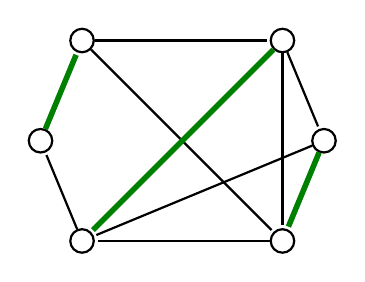
\begin{tikzpicture}[-,>=stealth,shorten >=1pt,auto,node distance=2cm, thick,main node/.style={scale=0.9,circle,draw,font=\sffamily\normalsize}]

            \node[] (x) []{};
            \node[main node] (1)[above left of = x] {};
            \node[main node] (2)[above right of = x] {};
            \node[main node] (3)[right of = x] {};
            \node[main node] (4)[below right of = x] {};
            \node[main node] (5)[below left of = x] {};
            \node[main node] (6)[left of = x] {};

            \path[every node/.style={font=\sffamily\small}]
                (1) edge (2)
                (2) edge (3)
                (3) edge[color = Green, line width = 2] (4)
                (4) edge (5)
                (5) edge (6)
                (6) edge[color = Green, line width = 2] (1)
                (1) edge (4)
                (2) edge (4)
                (3) edge (5)
                (2) edge[color = Green, line width = 2] (5)
                ;
        \end{tikzpicture}
        \caption{The green edges form a maximal matching of the graph.}
    \end{figure}

    Clearly, a maximal matching can be constructed in polynomial time through by simply adding edges until the property is preserved. In an even more efficient way, it can be computed by the following algorithm.

    \begin{algorithm}[H]
        \caption{The maximal matching algorithm}
        \textbf{Input:} an undirected graph $G$

        \textbf{Output:} a maximal matching $M$ of $G$
        \begin{algorithmic}[1]
            \Function{maximal-matching}{$G$}
                \State $M \gets \varnothing$
                \State $E' \gets E(G)$
                \While{$E' \neq \varnothing$}
                    \State Choose $e \in E'$
                    \State $S \gets S \cup \{e\}$
                    \State $E' \gets E' - \{f \in E' \mid e \cap f \neq \varnothing\}$
                \EndWhile
                \State Return $M$
            \EndFunction
        \end{algorithmic}
    \end{algorithm}

    We observe that the edges $e_1, \ldots, e_t$ picked by the algorithm are always a maximal matching: if $M = \{e_1, \ldots, e_t\}$ is not maximal then at least one edge could still get picked by the algorithm, meaning that it shouldn't have stopped.

    \begin{framedlem}{}
        Let $G$ be an undirected graph. For any matching $M$ of $G$ and any vertex cover $C$ of $G$ it holds that $\abs{M} \leq \abs{C}$. 
    \end{framedlem}

    \begin{proof}
        By definition, we observe that if $C$ is a vertex cover for $G$ then it is also a vertex cover for $G' = (V, E')$, where $E' \subseteq E(G)$. Hence, $C$ is also a vertex cover for any $G_M = (V,M)$, where $M$ is a matching of $G$. By definition of matching, in $G_M$ any vertex has either degree 0 or 1. Thus, each vertex of $C$ can cover at most one edge of $M$, meaning that $C$ has to have at least $\abs{M}$ vertices to cover all the edges of $M$.
    \end{proof}

    We observe that the lemma above is valid for any matching and any vertex cover, not only maximal and minimum ones, making it less specific for our situation. Nonetheless, we can use it to show that the following algorithm is actually a 2-approximation of VC.
    
    \begin{algorithm}[H]
        \caption{2-approximation of VC}
        \textbf{Input:} an undirected graph $G$

        \textbf{Output:} a vertex cover for $G$
        \begin{algorithmic}[1]
            \Function{2-approx-vc}{$G$}
                \State $M \gets \textsc{maximal-matching}(G)$
                \State Return $C = \bigcup\limits_{e \in M} e$
            \EndFunction
        \end{algorithmic}
    \end{algorithm}

    \begin{framedthm}{}
        Given a graph $G$, let $C^*$ be an optimal solution to $\mathrm{VC}(G)$. Given the output $C$ of \textsc{2-approx-vc}$(G)$, it holds that $\abs{C} \leq 2 \abs{C^*}$. 
    \end{framedthm}

    \begin{proof}
        Let $M = \{e_1, \ldots, e_t\}$ be the maximal matching returned by $\textsc{maximal-matching}(G)$. Since $\forall e,e' \in M$ it holds that $e \cap e' = \varnothing$ by definition of matching, it holds that $\abs{C} = 2 \abs{M}$. Hence, since $C^*$ is a vertex cover, by the previous lemma we get that $\abs{C} = 2 \abs{M} \leq 2 \abs{C^*}$.
    \end{proof}

    This result look quite easy, making us believe that this bound can be highly improved. However, it is conjectured that VC may be $\mathsf{NP}$-hard to approximate to any ratio $2-\varepsilon$ for any constant $\varepsilon > 0$ -- the Unique Games Conjecture implies this result, which is conjectured to be true. Hence, this simple approximation algorithm may actually be the best we can achieve.

    The vertex cover is also known to lie in the class of \textbf{Fixed-parameter Tractable (FPT)} problems, i.e the set of problems that can be solved in time $f(k) \cdot n^{O(1)}$, where $f$ is a computable function and $k$ is a fixed input parameter. We observe that, since $k$ is fixed, the value $f(k)$ becomes a \curlyquotes{constant}, making the running time polynomial with respect to the size of the input. The crucial part of the definition is to exclude functions of the form $f(k,n)$, such as $k^n$.
    
    \begin{algorithm}[H]
        \caption{Existence of a vertex cover}
        \textbf{Input:} an undirected graph $G$ an a non-negative integer $k$

        \textbf{Output:} True if $G$ has a vertex cover with at most $k$ vertices, False otherwise
        \begin{algorithmic}[1]
            \Function{VC}{$G,k$}
                \If{$E(G) \neq \varnothing$}
                    \State Return True
                \ElsIf{$k = 0$}
                    \State Return False
                \Else
                    \State Choose $\{u,v\} \in E(G)$
                    \If{$\textsc{VC}(G[V-\{u\}], k-1)$ or $\textsc{VC}(G[V-\{v\}], k-1)$}
                        \State Return True
                    \EndIf
                    \State Return False
                \EndIf
            \EndFunction
        \end{algorithmic}
    \end{algorithm}

    Here, the notation $G[V-\{u\}]$ corresponds to the \textbf{induced subgraph} by $V-\{u\}$ on $G$, i.e. the graph obtained by removing the vertices in $V-\{u\}$ from $G$ and all the edges that had one of such vertices as endpoints.

    \begin{frameddefn}{Induced subgraph}
        Given a graph $G$ and a subset $S \subseteq V(G)$, the subgraph induced by $S$ on $G$ is the graph $G[S] = (S, E')$ such that $E' = \{e \in E(G) \mid S \cap e \neq \varnothing\}$.
    \end{frameddefn}

    \begin{figure}[H]
        \centering

        \begin{tikzpicture}[-,>=stealth,shorten >=1pt,auto,node distance=2cm, thick,main node/.style={scale=0.9,circle,draw,font=\sffamily\normalsize}]

            \node[] (x) []{};
            \node[main node] (1)[fill = BlueLagoon, above left of = x] {};
            \node[main node] (2)[above right of = x] {};
            \node[main node] (3)[fill = BlueLagoon, right of = x] {};
            \node[main node] (4)[fill = BlueLagoon, below right of = x] {};
            \node[main node] (5)[fill = BlueLagoon, below left of = x] {};
            \node[main node] (6)[left of = x] {};

            \node[] (y) [right of = x, xshift = 175]{};
            \node[main node] (1y)[fill = BlueLagoon, above left of = y] {};
            \node[] (2y)[above right of = y] {};
            \node[main node] (3y)[fill = BlueLagoon, right of = y] {};
            \node[main node] (4y)[fill = BlueLagoon, below right of = y] {};
            \node[main node] (5y)[fill = BlueLagoon, below left of = y] {};
            \node[] (6y)[left of = y] {};

            \path[every node/.style={font=\sffamily\small}]
                (1) edge (2)
                (2) edge (3)
                (3) edge (4)
                (4) edge (5)
                (5) edge (6)
                (6) edge (1)
                (1) edge (4)
                (2) edge (4)
                (3) edge (5)
                (2) edge (5)

                (3y) edge (4y)
                (4y) edge (5y)
                (1y) edge (4y)
                (3y) edge (5y)
                ;
        \end{tikzpicture}
        \caption{The original graph (left) and the subgraph induced by the blue vertices (right).}
    \end{figure}

    To analyze the cost of the previous algorithm, we observe that the computational cost $T(n,m,k)$, where $n$ is the number of nodes and $m$ is the number of edges, is upper bounded by \[T(n,m,k) \leq 2T(n,m,k-1) + O(n+m)\]
    where $T(n,m,0) = T(n,0,k) = \Theta(1)$. Hence, we get that $T(n,m,k) = O(2^k (n+m))$. To get a more precise computational cost, we observe that if a graph $G$ has a vertex cover $C$ with $k$ vertices then $\abs{E(G)} \leq (n-1)k$ since in the worst case each of the $k$ vertices has degree $n-1$. Since $O(nk) = O(n)$ when $k$ is fixed, we get that $T(n,m,k) = O(2^kn)$.

    \chapter{Mathematical programming}

    \section{Approximations through Linear programming}

    Mathematical Programming involves using mathematical models and optimization techniques to solve problems that require finding the best solution from a set of possible choices, subject to constraints. It plays a key role in areas like operations research, artificial intelligence, machine learning, and systems design. In mathematical programming, an optimization problem is typically expressed as:
    \[
    \text{Minimize (or Maximize)} \quad f(x)
    \]
    subject to:
    \[
    g_i(x) \leq b_i \quad \forall i \in [m]
    \]
    \[
    h_i(x) = t_i \quad \forall i \in [m]
    \]
    \[
    x \in V
    \]
    Here, \( x \) is a vector of decision variables inside the vector space $V$ (usually $\Q^n$ or $\R^n$) and \( f(x) \) is an objective function, while \( g_i(x) \leq b_i\) and \( h_i(x) \leq t_i\)represent inequality and equality constraints. More specifically, we'll focus on \textbf{Linear Programming (LP)} and \textbf{Semi-Definite Programming (SDP)}. In linear programs, both the objective function and constraints are linear with respect to $\Q^n$ (or $\R^n$). Moreover, there is no equality constraints and each variable $x_i$ must be non-negative.
    \begin{figure}[H]
        \centering 
        \[\begin{split}
            \max x_1 + x_2 \\
            x_1 + 6x_2 & \leq 15 \\
            4x_1 - x_2 & \leq 10 \\
            x & \geq 0 \\
            x &\in \R^n
        \end{split}\]
        \caption{Example of a linear program.}
    \end{figure}

    \label{standard_lp}
    We observe that linear programs can be described in a compact matricial formulation.
    \begin{figure}[H]
        \centering 
        \[\begin{split}
            \max c^T x \\
            A x \leq b \\
            x  \geq 0 \\
            x \in \R^n
        \end{split}\]
        \caption{Standard matricial formulation of a linear program.}
    \end{figure}
    
    where $c \in \R^n, A \in \R^{m \times n}$ and $b \in \R^m$.
    \begin{figure}[H]
        \centering 
        \[\begin{split}
            \max \smat{1 & 1} \smat{x_1 \\ x_2} \\
            \smat{
                1 & 6 \\
                4 & -1 \\
                1 & -1
            } \smat{x_1 \\ x_2} &\leq \smat{15 \\ 10 \\ 1} \\
            x & \geq 0 \\
            x &\in \R^n
        \end{split}\]
        \caption{Matricial formulation of the previous a linear program example.}
    \end{figure}

    Linear programs can be solved in polynomial time. In particular, if a linear program has $n$ variables, $m$ constraints and each coefficient is representable as the ratio of two $t$-bits integers (real numbers get approximated as rational number) then the LP can be solved through the \textit{Ellipsoid method} in time $O((nmt)^c)$ for some $c > 0$ (this can be in someway extended also to SDPs). Even though it is theoretically guaranteed to have polynomial time, the Ellipsoid method becomes useful only for very large inputs. For more practical cases, the \textit{Simplex method} is used, which is based on \textit{pivot rules}. All of the pivot rules known for the Simplex method have a theoretical exponential lower bound through some particular programs that \curlyquotes{fool} the rule, but they have an average complexity that is way better than the Ellipsoid method. For our purposes, we do not care about how these methods work: we're only interested in knowing that LPs and SDPs can be solved in polynomial time.

    \textbf{Integer programs} are a particular type of linear program. Here, the vector space of interest is $\{0,1\}^n$. Lots of problem of common interested can be reduced to a linear program. For instance, given a graph $G$, consider the following integer program defined over the variables $x_{v_1}, \ldots, x_{v_n}$ where $V(G) = \{v_1, \ldots, v_n\}$.
    \begin{figure}[H]
        \centering 
        \[\begin{array}{ccc}
            \qquad\qquad\quad
            & \displaystyle \min \; \sum_{v \in V(G)} x_v \\\\
            & x_u + x_v \geq 1 & \forall \{u,v\} \in E(G) \\
            & x \in \{0,1\}^n
        \end{array}\]
        \caption{Integer program for the vertex cover problem.}
    \end{figure}

    Its easy to see that the above program perfectly describes the VC problem. In fact, the optimal integral solution to this IP actually gives us an optimal minimal vertex cover.
    
    \begin{framedlem}[label=ip_vc]{}
        Given a graph $G$, if $x^*$ is an optimal solution to the VC integer program then $C^* = \{v \mid v \in V(G), x^*_v = 1\}$ is a minimum vertex cover for $G$
    \end{framedlem}

    \begin{proof}
        Any feasible solution to the VC integer program corresponds to a vertex cover for $G$. In particular, in $C^*$ for all $\{u,v\} \in E(G)$ we have that: 
        \[\begin{array}{c}
           x^*_u + x^*_v \geq 1 \\
           x^*_u, x^*_v \in \{0,1\}
        \end{array} \iff x^*_u = 1 \lor x^*_v = 1 \iff u \in C^* \lor v \in C^*\]

        \textbf{Claim 1}: If $C'$ is a vertex cover for $G$ then there is a feasible $x'$ to the VP integer program such that $\sum_{v \in V(G)} x'_v = \abs{S}$.
        
        \begin{proof}[Proof of the claim.]
            Given a vertex cover $C'$, set $x'_v = 1$ if and only if $v \in S$. Then, since for all $\{u,v\} \in E(G)$ we have that $u \in S$ or $v \in S$, it must hold that $x_u = 1$ or $x_v = 1$, satisfying the constraint $x_u + x_v \geq 1$. Since each constraint is satisfied, $x'$ is a feasible solution. Moreover, by construction we have that $\sum_{v \in V(G)} x'_v = \abs{S}$.
        \end{proof}

        By way of contradiction, suppose that $C^*$ is not a minimum vertex cover. Then, there must be another vertex cover $V^\star$ such that $\abs{V^\star} < \abs{V^*}$. Thus, through the claim we know that there must another feasible solution $x^\star$ for which $\sum_{v \in V(G)} x^\star = \abs{V^\star} < \abs{V^*} = \sum_{v \in V(G)} x^*$, contradicting the fact that $x^*$ is optimal. Hence, $C^*$ must be a minimum vertex cover. 
    \end{proof}
    
    The above lemma implies that the Minimum Vertex Cover problem can be reduced to Integer programming. Hence, solving IPs is actually $\mathsf{NP}$-hard compared to solving LPs. This difference may seem counterintuitive: shouldn't the program be easier since we're working with way less feasible solutions? To give an intuition behind this hardness-gap, we can consider the fact that, since we're working over $\{0,1\}^n$ instead of $\Q^n$ or $\R^n$, we're intrinsically imposing lots of strong constrains over the space of feasible solutions, which becomes a lattice of integral vectors.

    Hence, IPs cannot be used to get perfect solutions. However, they can be used to get approximate solutions through \textbf{LP relaxation}. The idea is simple: we replace the constraints $x \in \{0,1\}^n$ and $x \geq 0$ with the constraints $x \in \R^n$ and $0 \leq x \leq 1$, transforming the IP into an LP.
    
    \begin{figure}[H]
        \centering 
        \[\begin{array}{ccc}
            \qquad\qquad\quad
            & \displaystyle \min \; \sum\limits_{v \in V(G)} x_v \\\\
            & x_u + x_v \geq 1 & \forall \{u,v\} \in E(G) \\
            & 0 \leq x \leq 1 & \\
            & x \in \R^n
        \end{array}\]
        \caption{LP relaxation for the vertex cover problem.}
    \end{figure}
    
    First of all, we observe that (generally) the space of feasible solution gets enlarged when the IP gets relaxed. In fact, every feasible solution to the original IP is a solution to the relaxed LP, but the optimal integral solution is not guaranteed to be an optimal solution to the LP. Moreover, we also observe that the optimal non-integral solution may not make sense for the original transformation.


    \begin{figure}[H]
        \centering

        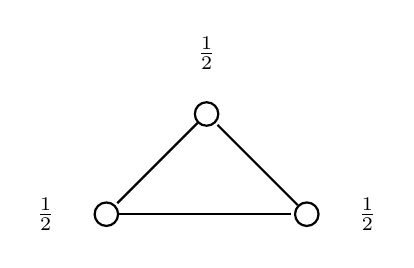
\begin{tikzpicture}[-,>=stealth,shorten >=1pt,auto,node distance=2cm, thick,main node/.style={scale=0.9,circle,draw,font=\sffamily\normalsize}]

            \node[main node] (1)[] {};
            \node[main node] (2)[below left of = 1] {};
            \node[main node] (3)[below right of = 1] {};

            \node[] (x)[above of = 1, yshift=-35] {$\frac{1}{2}$};
            \node[] (y)[left of = 2, xshift=35] {$\frac{1}{2}$};
            \node[] (z)[right of = 3, xshift=-35] {$\frac{1}{2}$};

            \path[every node/.style={font=\sffamily\small}]
                (1) edge (2)
                (2) edge (3)
                (3) edge (1)
                ;
        \end{tikzpicture}
        \label{vc_gap}
        \caption{The non-integral optimal solution for $K_3$ is $\overline{x} = \smat{\frac{1}{2} & \frac{1}{2} & \frac{1}{2}}^T$.}
    \end{figure}

    To fix this issue, the LP optimal solution is usually transformed into an approximate solution through techniques such as \textbf{rounding}. For instance, in the VS problem the rounding procedure is pretty obvious: in order for the constraints to be satisfied, for each edge at least one the two endpoints must have value greater than $\frac{1}{2}$. Hence, we select all the nodes that have value at least $\frac{1}{2}$. Surprisingly, this simple rounding procedure is guaranteed to yield a 2-approximation for the VC problem.
    
    \begin{framedthm}[label={vc_relax}]{}
        Given a graph $G$, if $\overline{x}$ is an optimal solution to the LP relaxation of the VC integer program then $\overline{C} = \{v \mid v \in V(G), \overline{x}_v \geq \frac{1}{2}\}$ is a 2-approximation for $\mathrm{VC}(G)$.
    \end{framedthm}

    \begin{proof}
        First of all, we observe that any feasible solution to the VC relaxed program still corresponds to a vertex cover for $G$. In particular, in $\overline{C}$ for all $\{u,v\} \in E(G)$ we have that: 
        \[\begin{array}{c}
           \overline{x}_u + \overline{x}_v \geq 1 \\
           0 \leq \overline{x}_u, \overline{x}_v \leq 1
        \end{array} \implies \overline{x}_u \geq \frac{1}{2} \lor \overline{x}_v \geq \frac{1}{2} \iff u \in \overline{C} \lor v \in \overline{C}\]

        \textbf{Claim:} $\abs{\overline{C}} \leq 2 \sum\limits_{v \in V(G)} \overline{x}_v$.

        \begin{proof}[Proof of the claim.]
            We observe that:
            \[\abs{\overline{C}} = \sum_{v \in \overline{C}} 1 \leq \sum_{v \in \overline{C}} 2 \overline{x}_v = 2 \sum_{v \in \overline{C}} \overline{x}_v \leq 2 \sum_{v \in V(G)} 2 \overline{x}_v\]
        \end{proof}

        Consider now an optimal solution $x^*$ to the IP version of the problem. Since $x^*$ is also a solution of the LP, but it isn't guaranteed to be optimal for the LP. Moreover,  through \Cref{ip_vc} we know that $x^*$ describes a minimum vertex cover $C^*$. Hence, we conclude that:
        \[\abs{\overline{C}} \leq  \sum_{v \in V(G)} 2 \overline{x}_v \leq  \sum_{v \in V(G)} 2 x^*_v = 2 \abs{C^*}\]
    \end{proof}

    \section{Integrality gap}

    In the proof of \Cref{vc_relax}, we were able to claim that the simple rounding procedure based on LP relaxation that we used gives us a vertex cover $\overline{C}$ such that $\abs{\overline{C}} \leq 2 \mathrm{LP}^*$, where $\mathrm{LP}^*$ is the optimal value of the objective function for the relaxation. If the claim inside the proof could be improved to $\abs{\overline{C}} \leq (2-\varepsilon) \mathrm{LP}^*$, we would get a better approximation ratio for the theorem since $\abs{\overline{C}} \leq (2-\varepsilon) \mathrm{IP}^*$ naturally follows from it. However, it can be show that the claim's bound is the best we can achieve through simple LP relaxation.
    
    In \Cref{ip_vc}, we showed how the solution $\overline{x} = \smat{\frac{1}{2} & \frac{1}{2} & \frac{1}{2}}^T$ is the optimal solution for the relaxed LP for the graph $K_3$. For the IP, instead, the solution $x^* = \smat{1 & 1 & 0}^T$ is clearly optimal for $K_3$. Hence, we get that $\mathrm{IP}^* = 2$ and $\mathrm{LP}^* = \frac{3}{2}$. Consider now a value $\alpha > 0$ such that $\abs{\overline{C}} \leq \alpha \mathrm{LP}^*$. Then, it must hold that:
    \[\alpha \geq \frac{2}{\frac{3}{2}} = \frac{4}{3}\]

    since otherwise we would get that:
    \[\abs{\overline{C}} \leq \alpha \mathrm{LP}^* < \frac{4}{3} \cdot \frac{3}{2} = 2 = \mathrm{IP}^*\]

    meaning that $\overline{C}$ would be a solution better than the optimal solution of the VC integer program, which is impossible. This result implies that there is an \textbf{integrality gap} $\alpha$ between the value of the optimal solution of the IP and the optimal solution of the relaxed LP.

    \begin{frameddefn}{Integrality gap}
        Given a problem $P$, consider the IP equivalent to $P$. Given an instance $I$ of $P$, let $\mathrm{IP}_P^*(I)$ and $\mathrm{LP}_P^*(I)$ be the optimal values of the IP and the LP relaxation of the IP for $I$. The integrality gap between between $\mathrm{IP}_P^*(I)$ and $\mathrm{LP}_P^*(I)$, denoted as $\mathrm{IG}_P(I)$, is defined as:
        \[\mathrm{IG}_P(I) = \frac{\mathrm{IP}_P^*(I)}{\mathrm{LP}_P^*(I)}\]

        The integrality gap for $P$, denoted as $\mathrm{IG}_P$, is defined as:
        \[\mathrm{IG}_P(I) = \sup_{I \in P} \mathrm{IG}_P(I) = \sup_{I \in P} \frac{\mathrm{IP}_P^*(I)}{\mathrm{LP}_P^*(I)}\]
    \end{frameddefn}

    \begin{framedprop}{Limits of LP relaxations}
        Given a problem $P$, let $\mathrm{ALG}_P$ be an algorithm that approximates $P$. Then:
        \begin{itemize}
            \item If $P$ is a minimization problem and $\mathrm{ALG}_P \leq \alpha \mathrm{LP}_P^*$ then $\alpha \geq \mathrm{IG}_P$
            \item If $P$ is a maximization problem and $\mathrm{ALG}_P \geq \alpha \mathrm{LP}_P^*$ then $\alpha \leq \mathrm{IG}_P$
        \end{itemize}
    \end{framedprop}

    \begin{proof}
        Assume that $P$ is a minimization problem. By way of contradiction, suppose that $\alpha < \mathrm{IG}_P$. Then, for any instance $I$ of $P$, it holds that:
        \[\mathrm{ALG}_P(I) \leq \alpha \mathrm{LP}^*(I) < \mathrm{IG}_P(I) \cdot \mathrm{LP}(I)_P^* = \frac{\mathrm{IP}_P^*(I)}{\mathrm{LP}_P^*(I)} \cdot \mathrm{LP}_P^*(I) = \mathrm{IP}^*_P(I)\]
        which is a contradiction. A similar argument can be made for the case where $P$ is a maximization problem.
    \end{proof}

    When the context makes it clear, we'll refer to $\mathrm{IG}_P, \mathrm{IP}_P^*$ and $\mathrm{LP}_P^*$ directly as $\mathrm{IG}, \mathrm{IP}^*$ and $\mathrm{LP}^*$. For the vertex cover problem, we showed that $\mathrm{IG}(K_3) = \frac{4}{3} = 2 - \frac{2}{3}$, meaning that $\mathrm{IG} \geq 2 - \frac{2}{3}$. By generalizing the argument to $K_n$, we can show that the integrality gap of the vertex cover problem is exactly $2$, meaning that $\forall \varepsilon > 0$ there can be no algorithm $\mathrm{ALG}$ such that $\mathrm{ALG} \leq (2-\varepsilon) \mathrm{LP}^*$ holds for all graphs.

    \begin{framedthm}{Integrality gap of VC}
        $\mathrm{IG}_\mathrm{VC} = 2$
    \end{framedthm}

    \begin{proof}
        We already know that the rounding procedure that we used is such that for all graphs $G$ it holds that $\mathrm{ALG}(G) \leq 2 \mathrm{LP}^*(G)$. Since the output of such rounding procedure is a (non-optimal) vertex cover, we know that $\mathrm{IP}^*(G) \leq \mathrm{ALG}(G)$. Hence, for all graphs $G$ we get that:
        \[\mathrm{IP}^*(G) \leq 2 \mathrm{LP}^*(G) \implies \frac{\mathrm{IP}^*(G)}{\mathrm{LP}^*(G)} \leq 2\]
        
        concluding that $\mathrm{IG} \leq 2$. Consider now the graph $K_n$. We observe that the vector $\overline{x}$ such that $x_v = \frac{1}{2}$ for all $v \in V(K_n)$ is a feasible solution for the LP relaxation of the VC problem. Hence, we know that:
        \[\mathrm{LP}^*(K_n) \leq \sum_{v \in V(K_n)} x_v = \frac{n}{2}\]

        \textbf{Claim:} any minimum vertex cover for $K_n$ has exactly $n-1$ nodes.

        \begin{proof}[Proof of the claim.]
            First, we show that there is a vertex cover of size $n-1$ for $K_n$. Let $C = \{x_1, \ldots, x_{n-1}\}$. For each edge $\{x_i, x_j\} \in E(K_n)$ with $i,j \in [n-1]$ we have that both $x_i, x_j$ are inside $C$. For each edge $\{x_i, x_n\} \in E(K_n)$ with $i \in [n-1]$, instead, we have that $x_i \in C$. Since every edge is covered by a vertex in $C$, $C$ is a vertex cover of size $n-1$.

            Suppose now by way of contradiction that there is a minimum vertex cover $C^*$ for $K_n$ of size $\abs{C^*} \leq n-2$. Then, we have that $\exists u,v \in V-C^*$ where $u,v$. Since $K_n$ is a $n$-clique, we have that $\{u,v\} \in E(K_n)$. However, we know that $u,v \notin C^*$, meaning that $C$ doesn't cover $\{u,v\}$ and thus that it isn't a vertex cover.
        \end{proof}

        The claim concludes that $\mathrm{IP}^* = n-1$, thus the integrality gap for $K_n$ is bounded by:
        \[\mathrm{IG}(K_n) = \frac{\mathrm{IP}^*(K_n)}{\mathrm{LP}^*(K_n)} \geq \frac{n-1}{\frac{n}{2}} = 2 - \frac{2}{n}\]

        Hence, we conclude that:
        \[\mathrm{IG} = \sup_{G} \mathrm{IG}(G) \geq \sup_{n \in \N} \mathrm{IG}(K_n) \geq \lim_{n \to +\infty} \; 2 - \frac{2}{n} = 2\]

    \end{proof}

    Even thought the above propositions only refers to algorithms that are bounded by linear relaxations, meaning that other algorithms may indeed produce a better approximation ratio, for many problems we conjecture that the integrality gap is actually the best possible approximation ratio of any algorithm for the problem. For instance, it is conjectured that there is no $(2-\varepsilon)$-approximation of the VC problem unless $\mathsf{P} \neq \mathsf{NP}$, even thought no one has yet proven such result.

    \newpage

    \subsection{The Minimum Set Cover problem}

    In the previous section we were able to show that the integrality gap of the minimum vertex cover can be exactly computed, concluding that $\mathrm{IG}_{\mathrm{VC}} = 2$. However, the integrality gap cannot be always nicely computed. Nonetheless, finding upper and lower bounds to it still allows us know if our rounding procedure is good enough or not. This is the case of the \textbf{Minimum Set Cover} problem.

    Given a number $n \in N$, let $\mathcal{U} = [n]$ be the universe set and let $\mathcal{C} = \{S_1, \ldots, S_m\}$ be a collection of subsets $S_i \subseteq \mathcal{U}$. The SC problems asks us to find the smallest sub-collection $\mathcal{S} \subseteq \mathcal{C}$ such that:
    \[\mathcal{U} = \bigcup_{S_j \in \mathcal{S}} S_j\]
    
    For instance, given $\mathcal{U} = [4]$ and $S_1 = \{1,2\}, S_2 = \{2,3\}, S_3 = \{3,4\}$, the smallest set cover is given by $\mathcal{S} = \{S_1, S_3\}$. It's easy to see that the VC problem can be reduced to the SC problem by considering the universe set $\mathcal{U} = [\abs{E(G)}]$ and the collection $\mathcal{C} = \{S_{v_1}, \ldots, S_{v_n}\}$ where $S_{v_i} = \{i \in [\abs{E(G)}] \mid v_i \in e_i\}$, making the SC problem $\mathsf{NP}$-hard. The IP program equivalent to the SC problem can be obtained by imposing constraints similar to the ones of the VC problem over the variables $x_1, \ldots, x_m$, where $x_j = 1$ if and only if $j$ is selected in the output cover.

    \begin{figure}[H]
        \centering 
        \[\begin{array}{ccc}
            \qquad\qquad\quad
            & \displaystyle \min \; \sum_{j \in [m]} x_j \\\\
            & \displaystyle \sum_{\substack{j \in [m] \\ \text{ s.t. } i \in S_j}} x_j \geq 1 & \forall i \in [n] \\
            & x \in \{0,1\}^m
        \end{array}\]
        \caption{Integer program for set cover problem.}
    \end{figure}

    We observe that the $\frac{1}{2}$ rounding rule that we used on the optimal solution of the LP relaxation of vertex cover cannot be used for the LP relaxation of set cover. In the VC problem, we had constraints of the form $x_u + x_v \geq 1$, which imply that:
    \[\max(x_u, x_v) \geq \frac{x_u + x_v}{2} \geq \frac{1}{2}\]

    guaranteeing that at least one between $x_u$ and $x_v$ can be rounded to 1. Here, we have constraints of the form $\sum_{\substack{j \in [m] \\ \text{ s.t. } i \in S_j}} x_j \geq 1$, which imply that:
    \[\max(x_{j_1}, \ldots, x_{j_k}) \geq \frac{x_{j_1} + \ldots + x_{j_k}}{k} \geq \frac{1}{k}\]

    where $j_1, \ldots, j_k$ are the indexed in $[m]$ for which $i \in S_{j_h}$. Thus, there is no guarantee of at least one between $x_{j_1}, \ldots, x_{j_j}$ to be rounded to 1. This means that we need a new rounding rule for such problem. In particular, we'll use a \textbf{randomized rounding rule}, which, surprisingly, is the best for most problems.

    \begin{algorithm}[H]
        \caption{Randomized rounding for SC}
        \textbf{Input:} an universe set $\mathcal{U}$ and a collection $\mathcal{C}$

        \textbf{Output:} a set cover $A$ for $\mathrm{U}$
        \begin{algorithmic}[1]
            \Function{randomized-rounding-SC}{$\mathcal{U}, \mathcal{C}$}
                \State $A \gets \varnothing$
                \State $\overline{x} \gets \mathrm{LP}_{\mathrm{SC}}^*(\mathcal{U}, \mathcal{S})$
                \For{$k \in [\ceil{2 \ln n}]$}
                    \State $A_k \gets \varnothing$
                    \For{$j \in [m]$}
                        \State Flip a coin with head probability set to $\overline{x_j}$ and set $c_{k,j}$ as the outcome
                        \If{$c_{k,j} = 1$}
                            \Comment{1 is heads, 0 is tails}
                            \State $A_k \gets A_k \cup \{S_j\}$
                        \EndIf
                    \EndFor
                    \State $A \gets A \cup A_k$
                \EndFor
                \State Return $A$
            \EndFunction
        \end{algorithmic}
    \end{algorithm}

    \begin{framedlem}{}
        Let $(\mathcal{U}, \mathcal{C})$ be an input of the SC problem. Given the output $\mathcal{S}$ of \textsc{randomized-rounding-sc}$(\mathcal{U}, \mathcal{C})$, it holds that:
        \[\Pr \sbk{\mathcal{U} \text{ covered by } A}  = 1-\frac{1}{n}\]
    \end{framedlem}

    \begin{proof}
        Fix an iteration $k \in [\ceil{2 \ln n}]$ of the outer for loop and fix an element $i \in [n]$. Recalling that $\forall x \in \R$ it holds that $1-x \leq e^{-x}$, we observe that:
        \[\begin{split}
            \Pr[i \text{ not cov. by } A_k] = \prod_{\substack{j \in [m] \\ \text{s.c. } i \in S_j}} 1-\overline{x}_j \leq \prod_{\substack{j \in [m] \\ \text{s.c. } i \in S_j}} e^{-\overline{x}_j} \leq \exp\rbk{-\sum_{\substack{j \in [m] \\ \text{s.c. } i \in S_j}} \overline{x}_j}\\
        \end{split}\]

        Since $\overline{x}$ is a solution to $\mathrm{LP}_{SC}$, we have that:
        \[\begin{split}
            \Pr[i \text{ not cov. by } A_k] \leq \exp \rbk{-\sum_{\substack{j \in [m] \\ \text{s.c. } i \in S_j} } \overline{x}_j} \leq e^{-1}
        \end{split}\]

        Since $A = A_1 \cup \ldots \cup A_k$, by iterating over all $k \in [\ceil{2 \ln n}]$ the probability of $i$ not being covered by $A$ is bounded by:
        \[\begin{split}
            \Pr[i \text{ not cov. by } A] &= \Pr[\forall k \;\; i \text{ not cov. by } A_k] \leq \prod_{k \in [\ceil{2 \ln n}]} e^{-1} = e^{- \ceil{2 \ln n}} \leq e^{- 2 \ln n} = \frac{1}{n^2}
        \end{split}\]

        Finally, by iterating over all $i \in [n]$, we get that:
        \[\Pr[\mathcal{U} \text{ not cov. by } A] = \Pr[\exists i \in [n] \;\; i \text{ not cov. by } A] \leq \sum_{i \in [n]} \Pr[i \text{ not cov. by } A] \leq\frac{1}{n}\]
    \end{proof}

    The above lemma guarantees with enough probability that the output of the randomized rounding rule is indeed a set cover -- recall that we're interested to solve the problem for large values of $n$. We'll now show that the expected value of the solution is not so bad.

    \begin{framedlem}{}
        Let $(\mathcal{U}, \mathcal{C})$ be an input of the SC problem. Given the output $\mathcal{S}$ of \textsc{randomized-rounding-sc}$(\mathcal{U}, \mathcal{C})$, it holds that:
        \[\Exp[\abs{A}] \leq \ceil{2 \ln n} \mathrm{IP}^*\]
    \end{framedlem}

    \begin{proof}
        Fix an iteration $k \in [\ceil{2 \ln n}]$. We observe that:
        \[\Exp[\abs{A_k}] = \sum_{j \in [m]} \Pr[S_j \in A_k] = \sum_{j \in [m]} \overline{x}_j = \mathrm{LP}^*\]
        Since $A = A_1 \cup \ldots \cup A_k$, by linearity of the expected value operator we get that:
        \[\Exp[ \abs{A}] \leq \Exp\sbk{\sum_{k \in [\ceil{2 \ln n}]} \abs{A_k}} = \sum_{k \in [\ceil{2 \ln n}]} \Exp\sbk{\abs{A_k}} = \ceil{2 \ln n} \mathrm{LP}^* \leq \ceil{2 \ln n} \mathrm{IP}^*\]
    \end{proof}

    Since through the above lemma we have implicitly proven that $\Exp[\abs{A}] \leq \ceil{2 \ln n} \mathrm{LP}^*$, through the law of large numbers we know that if for each pair $(\mathcal{U}, \mathcal{C})$ we repeatedly compute the algorithm \text{randomized-rounding-sc} we will, eventually, get an output $A'$ such that $\abs{A'} \leq  \ceil{2 \ln n} \mathrm{LP}^*$. Since $\mathrm{IP}^* \leq \abs{A'}$, we get that:
    \[\mathrm{IG}_{\mathrm{SC}} \leq \ceil{2 \ln n}\]

    Moreover, we observe that the algorithm can be modified to get a better bound. By simply replacing the number of iterations of the outer loop with $\ceil{(1+\varepsilon) \ln n}$, for any $\varepsilon > 0$, we get that $\Exp[\abs{A}] \leq \ceil{(1+\varepsilon) \ln n} \mathrm{LP}^*$, even though we would also have that $\Pr \sbk{\mathcal{U} \text{ covered by } A}  = 1-n^{-\varepsilon}$, which is worse for small values of $\varepsilon$ -- this probability can still be boosted by repeatedly computing the output. Hence, actually get that:
    \[\mathrm{IG}_{\mathrm{SC}} \leq \ceil{\ln n}\]

    To show a lower bound on the integrality gap of set cover, we proceed in a way similar to what we did for the vertex cover problem. However, in this case we're not able to show a tight bound. The result is due to \textcite{ig_sc}.
    
    \begin{framedthm}{Integrality gap of SC}
        For any $n \in \N$ it holds that:
        \[\frac{1}{4 \ln 2} \; \ln n \leq \mathrm{IG}_{\mathrm{SC}} \leq \ceil{\ln n}\]
    \end{framedthm}

    \begin{proof}
        We have already showed that $\mathrm{IG}_{\mathrm{SC}} \leq \ceil{\ln n}$, hence proving the lower bound suffices. Fix $n \in \N$ and let $m \in \N$ be the even number such that $n = \binom{m}{\frac{m}{2}}$. We observe that:
        \[n = \binom{m}{\frac{m}{2}} = \Theta \rbk{\frac{2^m}{\sqrt{m}}} \implies m = \log n - \Theta(\log \log n)\]
        
        Let $\mathcal{U}_n$ be the set of all elements representing a subset of $[m]$ with $\frac{m}{2}$ elements:
        \[\mathcal{U}_n = \{e_a \mid A \in \binom{[m]}{\frac{m}{2}}\}\]

        Let $\mathcal{C}_n = \{S_1, \ldots, S_m\}$, where $S_i = \{e_A \in \mathcal{U}_n \mid i \in A\}$.

        \textbf{Claim 1}: $\mathrm{LP}^*(\mathcal{U}_n, \mathcal{C}_n) \leq 2$

        \begin{proof}[Proof of Claim 1.]
            First, we observe that, by construction, every element $e_A \in \mathcal{U}_n$ is in exactly $\abs{A}$ sets. Hence, given the vector $x = \smat{\frac{2}{m} & \cdots & \frac{2}{m}}^T$ for each $e_A \in \mathcal{U}_n$ we have that:
            \[\sum_{\substack{j \in [m] \\ \text{s.t. } e_A \in S_j}} x_j = \sum_{\substack{j \in [m] \\ \text{s.t. } e_A \in S_j}} \frac{2}{m} = \abs{A} \; \frac{2}{m} = 1\]
            meaning that $x$ is a feasible solution for $\mathrm{LP}^*(\mathcal{U}_n, \mathcal{C}_n)$ with objective value $2$.
        \end{proof}

        \textbf{Claim 2:}  $\mathrm{IP}^*(\mathcal{U}_n, \mathcal{C}_n) \geq \frac{1}{2} \; \log n - O(\log log n)$

        \begin{proof}[Proof of Claim 2.]
            By way of contradiction, suppose that there is a sub-collection $\mathcal{S} = \{S_{i_k}, \ldots, S_{i_k}\}$ with $k \leq \frac{m}{2}$ that covers $\mathcal{U}_n$. Given $T = [m] - \{i_1, \ldots, i_k\}$, it holds that $\abs{T} \geq m - \frac{m}{2} = \frac{m}{2}$. Hence, we can always find a subset $A \subseteq T$ such that $\abs{A} = \frac{m}{2}$. Since $A \subseteq T$, we have that $e_A \notin S_{i_1} \cup \ldots \cup S_{i_k}$, contradicting the fact that $\mathcal{S}$ is a cover of $\mathcal{U}_n$.

            Hence, there for any set cover $\mathcal{S}$ of $(\mathcal{U}_n, \mathcal{C}_n)$ it must hold that
            \[\abs{\mathcal{S}} > \frac{m}{2} = \frac{1}{2}\log n - \Theta(\log \log n) \implies \mathrm{IP}^* \geq \frac{m}{2} = \frac{1}{2}\log n - O(\log \log n)\]

            \textit{Note}: the asymptotic notation changes from $\Theta$ to $O$ due to the less than constraint
        \end{proof}
        
        From the two claims we get that:
        \[\mathrm{IG} = \sup_{(\mathcal{U}, \mathcal{C})} \mathrm{IG}(\mathcal{U}, \mathcal{C}) \geq \max_{n \in \N} \mathrm{IG}(\mathcal{U}_n, \mathcal{C}_n) \geq \max_{n \in \N} \; \frac{\frac{1}{2}\log n - O(\log \log n)}{2}\]
        
        which can happen only if:
        \[\mathrm{IG} = \sup_{(\mathcal{U}, \mathcal{C})} \mathrm{IG}(\mathcal{U}, \mathcal{C}) \geq \frac{1}{4} \;\log n = \frac{1}{4 \ln 2} \; \ln n\]
    \end{proof}

    \subsection{The Densest Subgraph problem}

    The \textbf{Densest Subgraph} problem asks to find a non-empty subset of vertices $S$ in a given graph $G$ whose induced subgraph $G[S]$ maximizes a measure of \textbf{density} $\rho(S)$, defined as the ratio between the number of edges in $G[S]$ and the number of vertices in $S$.
    \[\rho(S) = \frac{{\abs{E(G[S])}}}{\abs{S}}\]

    \begin{figure}[H]
        \centering

        \begin{tikzpicture}[-,>=stealth,shorten >=1pt,auto,node distance=2cm, thick,main node/.style={scale=0.9,circle,draw,font=\sffamily\normalsize}]

            \node[] (x) []{};
            \node[main node] (1)[fill = BlueLagoon, above left of = x] {};
            \node[main node] (2)[above right of = x] {};
            \node[main node] (3)[fill = BlueLagoon, right of = x] {};
            \node[main node] (4)[fill = BlueLagoon, below right of = x] {};
            \node[main node] (5)[fill = BlueLagoon, below left of = x] {};
            \node[main node] (6)[left of = x] {};

            \path[every node/.style={font=\sffamily\small}]
                (1) edge (2)
                (2) edge (3)
                (3) edge (4)
                (4) edge (5)
                (5) edge (6)
                (6) edge (1)
                (1) edge (4)
                (2) edge (4)
                (3) edge (5)
                (2) edge (5)
                ;
        \end{tikzpicture}
        \caption{The subgraph induced by the blue nodes has density $\frac{4}{3}$}
    \end{figure}

    The Densest Subgraph problem became of particular interest in the '00s, mostly in Social Networks. For instance, companies such as Google used dense subgraphs to cut off \textit{spam-networks}, i.e. website networks that used to spam-link each other in order to boost their ranking for the PageRank algorithm used by Google to recommend websites. We observe that the densest subgraph problem is equivalent to the \textbf{Maximum Average Degree Subgraph} problem:
    \[\argmax_{S \subseteq V} \frac{{\abs{E(G[S])}}}{\abs{S}} = \argmax_{S \subseteq V} \frac{{\abs{E(G[S])}}}{\abs{S}} = \argmax_{S \subseteq V} \frac{\sum\limits_{v \in S} \deg_{G[S]}(v)}{2\abs{S}} = \argmax_{S \subseteq V} \frac{\sum\limits_{v \in S} \deg_{G[S]}(v)}{\abs{S}}\]

    This equivalence between the two problems allows us to formulate the following IP representation of the problem, where each variable $x_{i,j}$ corresponds to an edge $\{i,j\} \in E(G)$ and each variable $y_i$ corresponds to a vertex $i \in V(G)$.

    \begin{figure}[H]
        \centering 
        \[\begin{array}{ccc}
            \qquad\qquad\quad
            & \displaystyle \max \; \frac{\sum_{\{i,j\} \in E(G)} x_{i,j}}{\sum_{i \in V(G)} y_i} \\\\
            & x_{i,j} \leq y_i & \forall \{i,j\} \in E(G) \\
            & x_{i,j} \leq y_j & \forall \{i,j\} \in E(G) \\
            & \displaystyle \sum_{\substack{i \in V(G)}} y_i \leq 1 & \\
            & x \in \{0,1\}^{m} \\
            & y \in \{0,1\}^{n}
        \end{array}\]
        \caption{Integer program for densest subgraph problem.}
    \end{figure}

    To get a more standard looking IP program, we can normalize the variables in the following way.

    \begin{figure}[H]
        \centering 
        \[\begin{array}{ccc}
            \qquad\qquad\quad
            & \displaystyle \max \; \sum_{\{i,j\} \in E(G)} x_{i,j} \\\\
            & x_{i,j} \leq y_i & \forall \{i,j\} \in E(G) \\
            & x_{i,j} \leq y_j & \forall \{i,j\} \in E(G) \\
            & \displaystyle \sum_{\substack{i \in V(G)}} y_i \leq 1 & \\
            & x \in \{0,1\}^{m} \\
            & y \in \{0,1\}^{n}
        \end{array}\]
        \caption{Normalized integer program for densest subgraph problem.}
        \label{ds_normalized}
    \end{figure}

    \textcite{charikar} proved that the integrality gap of this normalized version is 1, meaning that $IP_{\mathrm{DS}}^* = LP^*_{\mathrm{DS}}$. To show this, we prove the two following lemmas.

    \begin{framedlem}[label={ig_ds_1}]{}
        Let $G$ be a graph. Then, for each subset $S \subseteq V(G)$ there is a feasible solution to $LP_{\mathrm{DS}}(G)$ with objective value equal to $\rho(S)$.
    \end{framedlem}

    \begin{proof}
        Given $S \subseteq V(G)$, let $\overline{x}, \overline{y}$ be defined as:
        \[\overline{x_{i,j}} = \soe{ll}{
            \frac{1}{\abs{S}} & \text{if } \{i,j\} \in S \\
            0 & \text{otherwise}\\
        } \qquad \qquad \overline{y_i} = \soe{ll}{
            \frac{1}{\abs{S}} & \text{if } \{i,j\} \in E(G[S]) \\
            0 & \text{otherwise}\\
        }\]

        \textbf{Claim:} $\overline{x}, \overline{y}$ is a feasible solution

        \begin{proof}[Proof of the claim.]
            By construction, we have that:
            \[\sum_{\substack{i \in V(G)}} y_i = \sum_{i \in S} y_i + \sum_{i \in \overline{S}} y_i = \sum_{i \in S} \frac{1}{\abs{S}} + \sum_{i \in \overline{S}} 0 = 1\]
            hence the third constraint is satisfied. For each edge $\{i,j\} \in E(G)$, if $\{i,j\} \in E(G[S])$ then $i,j \in S$, implying that $x_i = y_i = y_j = \abs{\frac{1}{S}}$. If $\{i,j\} \notin E(G[S])$, instead, we have that $x_{i,j} = 0 \leq y_i, y_j$. In both cases, the constraints are satisfied.
        \end{proof}

        Finally, we observe that the objective value of $\overline{x}, \overline{y}$ is equal to the density of $S$:
        \[\sum_{\{i,j\} \in E(G)} x_{i,j} = \sum_{\{i,j\} \in E(G[S])} x_{i,j} + \sum_{\{i,j\} \in E(G)-E(G[S])} x_{i,j} = \frac{\abs{E(G[S])}}{\abs{S}} = \rho(S)\]

    \end{proof}

    \begin{framedlem}[label={ig_ds_2}]{}
        Let $G$ be a graph. Then, for each feasible solution to $LP_{\mathrm{DS}}(G)$ with objective value $v$, there is a subset $S \subseteq V(G)$ such that $\rho(S) \geq v$
    \end{framedlem}

    \begin{proof}
        Let $x',y'$ be any feasible solution to $LP_{\mathrm{DS}}(G)$. We observe that this solution may have some \curlyquotes{slack} from the constraints, meaning that they are not satisfied at equality. To make things easier, we can transform the solution $x',y'$ to a new solution objective value at least $v$ and without slack. To achieve this, let $\overline{x}, \overline{y}$ such that $\overline{y_i} = y'_i$ for all $i \in V(G)$ and $\overline{x_{i,j}} = \min(y'_i, y'_j)$ for all $\{i,j\} \in E(G)$.

        \textbf{Claim 1:} $\overline{x}, \overline{y}$ is a feasible solution with objective value at least $v$
        
        \begin{proof}[Proof of Claim 1.]
            Since $x',y'$ is a feasible solution, it satisfies the constraints of the LP. Hence, we get that:
            \[\sum_{\substack{i \in V(G)}} \overline{y}_i = \sum_{\substack{i \in V(G)}} y'_i \leq 1\]
            and that:
            \[x_{i,j} = \min(y'_i, y'_j) \leq y_i', y_j'\]

            for each $\{i,j\} \in E(G)$. Moreover, also by feasibility of $x',y'$, we have that:
            \[\sum_{\{i,j\} \in E(G)} \overline{x}_{i,j} = \sum_{\{i,j\} \in E(G)} \min(y_i', y_j') \geq \sum_{\{i,j\} \in E(G)} x'_{i,j} = v\]
        \end{proof}

        For each $r \in \R$, let $S(r) = \{i \mid \overline{y}_i \geq r\}$ and let $E(r) = \{\{i,j\} \mid \overline{x}_{i,j} \geq r\}$.

        \textbf{Claim 2:} $\{i,j\} \in E(r)$ if and only if $i,j \in S(r)$, i.e. $E(r) = E(G[S(r)])$

        \begin{proof}[Proof of Claim 2.]
            If $\{i,j\} \in E(r)$, we have that:
            \[r \leq \overline{x_{i,j}} = \min(y'_i, y'_j) \leq \overline{y'}_i, \overline{y'}_j\]
            hence $i,j \in S(r)$. Vice versa, if $i,j \in S(r)$ then:
            \[r \leq \min(\overline{y}_i, \overline{y}_j) = \min(y'_i, y'_j) = \overline{x_{i,h}}\]
            hence $\{i,j\} \in E(r)$.
        \end{proof}

        Now, things will get pretty strange and seemingly pointless -- don't worry, keep going with the flow. Let $\pi$ be a permutation of indices that orders $y_1, \ldots, y_n$ in ascending order:
        \[0 \leq \overline{y}_{\pi(1)} \leq \ldots \leq \overline{y}_{\pi(n)}\]
        In other words, $\pi$ is a permutation that sorts $\overline{y}$ in ascending order. Consider now the following integral:
        \[\int_{0}^{\overline{y}_{\pi(n)}} \abs{S(r)} \, dr\]

        We notice that, for each $r \in \R$ such that $0 \leq r \leq \overline{y}_{\pi(1)}$ it holds that $\abs{S(r)} = n$. Similarly, for each $r \in R$ such that $\overline{y}_{\pi(1)} < r \leq \overline{y}_{\pi(2)}$ it holds that $\abs{S(r)} = n-1$, and so on (see \Cref{int_ds} below). Hence, we have that:
        \[\begin{split}
            \int_{0}^{\overline{y}_{\pi(n)}} \abs{S(r)} \, dr &= \int_{0}^{\overline{y}_{\pi(1)}} \abs{S(r)} \, dr + \int_{\overline{y}_{\pi(1)}}^{\overline{y}_{\pi(2)}} \abs{S(r)} \, dr + \ldots + \int_{\overline{y}_{\pi(n-1)}}^{\overline{y}_{\pi(n)}} \abs{S(r)} \, dr \\
            &= \int_{0}^{\overline{y}_{\pi(1)}} n \, dr + \int_{\overline{y}_{\pi(1)}}^{\overline{y}_{\pi(2)}} n-1 \, dr + \ldots + \int_{\overline{y}_{\pi(n-1)}}^{\overline{y}_{\pi(n)}} 1 \, dr \\
            &= n(\overline{y}_{\pi(1)}-0) + (n-1)(\overline{y}_{\pi(2)}-\overline{y}_{\pi(1)}) + \ldots + (\overline{y}_{\pi(n)}-\overline{y}_{\pi(n-1)}) \\
            &= \overline{y}_{\pi(1)}(n-(n-1)) + \ldots + \overline{y}_{\pi(n)}(2-1) \\
            &= \overline{y}_{\pi(1)} + \ldots + \overline{y}_{\pi(n)} \\
            &= y'_1 + \ldots + y'_n \\
            &\leq 1
        \end{split}\]

        Proceeding in a similar way, we get that:
        \[\begin{split}
            \int_{0}^{\overline{y}_{\pi(n)}} \abs{E(r)} \, dr = \sum_{\{i,j\} \in E(G)} x_{i,j} \geq v \\
        \end{split}\]

        \textbf{Claim 3:} there is an $r \in \R$ with $0 \leq r \leq \overline{y}_{\pi(n)}$ such that $\abs{E(r)} \geq v \abs{S(r)}$

        \begin{proof}{Proof of Claim 3.}
            By way of contradiction, suppose that for all $r \in \R$ with $0 \leq r \leq \overline{y}_{\pi(n)}$ it holds that $\abs{E(r)} < v \abs{S(r)}$. Then, the two previous integrals are bounded in the following way:
            \[v \leq \int_{0}^{\overline{y}_{\pi(n)}} \abs{E(r)} \, dr <  \int_{0}^{\overline{y}_{\pi(n)}} v \abs{S(r)} \, dr \leq v\]
            raising a contradiction.
        \end{proof}

        Let $r^*$ be a value satisfying Claim 3. Then, we have that:
        \[\rho(S(r^*)) = \frac{\abs{E(G[S(r^*)])}}{\abs{S(r^*)}} = \frac{\abs{E(r^*)}}{\abs{S(r^*)}} \geq v\]

    \end{proof}

    \begin{figure}[H]
        \centering
        \begin{tikzpicture}[scale=0.7]
            \draw[-stealth] (-0.5,0) -- (2,0) node[below]{$\overline{y}_{\pi(1)}$} -- (4,0) node[below]{$\overline{y}_{\pi(2)}$} -- (7,0) node[below]{$\cdots$} -- (10,0) node[below]{$\overline{y}_{\pi(n - 2)}$} -- (12,0) node[below]{$\overline{y}_{\pi(n - 1)}$} -- (14,0) node[below]{$\overline{y}_{\pi(n)}$} -- (15,0) node[right]{$r$};
            \draw[-stealth] (0,-0.5) -- (0,0) node[below left]{0} -- (0,1) node[left]{1} -- (0,2) node[left]{2} -- (0,3.5) node[left]{$\cdots$} -- (0,5) node[left]{$n - 1$} -- (0,6) node[left]{$n$} -- (0,7.5) node[above]{$\abs{S(r)}$};
            \draw[thick, orange] (0,6) -- (2,6) -- (2,5) -- (4,5) -- (4, 4) -- (5,4);
            \draw[dashed, orange] (5,4) -- (6,4);
            \draw[dashed, orange] (9,3) -- (8,3);
            \draw[thick, orange] (14,0) -- (14,1) -- (12,1) -- (12,2) -- (10,2) -- (10,3) -- (9,3);
        \end{tikzpicture}
        \caption{Plot of the value $\abs{S(r)}$ with increasing values of $r$ }
        \label{int_ds}
    \end{figure}

    \begin{framedthm}{Integrality gap of DS}
        $\mathrm{IG}_{\mathrm{DS}} = 1$
    \end{framedthm}

    \begin{proof}
        Follows from \Cref{ig_ds_1} and \Cref{ig_ds_2}.
    \end{proof}
    
    We observe that the above theorem implies only that the optimal value of the IP and the LP relaxation is equal, not that every solution to the LP is an maximum densest subgraph. In fact, the optimal solution of the LP found by the Ellipsoid method or the Simplex method may be fractional: every optimal integral solution is also an optimal linear solution, but not vice versa. Hence, we still need to apply some rounding procedure. Luckily, the proof of \Cref{ig_ds_2} implicitly gives us a perfect rounding procedure, one for which the output value is perfectly optimal and non-approximated.
    
    \begin{algorithm}[H]
        \caption{Charikar's optimal program for the DS problem}
        \textbf{Input:} an undirected graph $G$

        \textbf{Output:} the densest subgraph of $G$ 
        \begin{algorithmic}[1]
            \Function{densest-subgraph}{$G$}
                \State $\overline{x}, \overline{y} \gets \mathrm{LP}^*_{\mathrm{DS}}(G)$
                \State $S \in \argmax\limits_{i \in [n]} \rho(S(\overline{y}_i))$
                \State Return $G[S]$
            \EndFunction
        \end{algorithmic}
    \end{algorithm}

    Even thought this program is optimal, polynomial-time and deterministic, its runtime is actually $O(n^9)$, making it \textbf{unusable} for real applications such as spam-network detection, where the input graph has more than $10^24$ vertices. 

    \section{Approximations through duality}

    As we discussed, LPs can be solved in polynomial time through the Ellipsoid method. However, such polynomial is way too high to make it practical. For instance, Charikar's optimal algorithm for the DS problem has a runtime of $O(n^9)$, making this approach impractical for large graphs. To fix this issue, \textcite{charikar} developed a greedy $\frac{1}{2}$-approximation for the problem that actually runs in $O(n)$. The idea used by Charikar is based on the concept of \textbf{linear program duality}.

    Consider a maximization problem in standard matricial form (see \Cref{standard_lp}) 
    \begin{figure}[H]
        \centering 
        \[\begin{split}
            \max c^T x \\
            A x \leq b \\
            x  \geq 0 \\
            x \in \R^n
        \end{split}\]
    \end{figure}
    
    The \textbf{dual} of such problem is the linear program defined as:
    \begin{figure}[H]
        \centering 
        \[\begin{split}
            \max b^T y \\
            A^T y \geq c \\
            y  \geq 0 \\
            y \in \R^m
        \end{split}\]
    \end{figure}

    while the original program is referred to as the \textbf{primal}.

    \begin{figure}[H]
        \centering
        \[\begin{array}{ccc}
            \begin{array}{c}
                \max \; \smat{2 & 3} \smat{x_1 \\ x_2} \\
                \begin{split}
                    \smat{
                        4 & 8 \\
                        2 & 1 \\
                        3 & 2 
                    }
                    \smat{
                        x_1 \\ x_2
                    } &\leq
                    \smat{
                        12 \\ 3 \\ 4
                    }
                    \\
                    x_1, x_2 &\geq 0
                \end{split}
            \end{array}
                

            &\qquad\qquad\qquad\qquad&

            \begin{array}{c}
                \min \; \smat{12 & 3 & 4} \smat{y_1 \\ y_2 \\ y_3} \\
                \begin{split}
                    \smat{
                        4 & 2 & 3 \\
                        8 & 1 & 2
                    }
                    \smat{
                        y_1 \\ y_2 \\ y_3
                    } \geq
                    \smat{
                        2 \\ 3
                    }
                    \\
                    y_1, y_2, y_3 \geq 0
                \end{split}
            \end{array}
        \end{array}\]
        \caption{Example of a primal program (left) and its dual program (right).}
    \end{figure}
    
    We observe that the dual of the dual program is the primal program. Duality plays a fundamental role in linear programming and algorithm design. For the former, the importance comes from the \textbf{Weak Duality Theorem}.

    \begin{framedthm}{Weak Duality Theorem}
        Let $(P,D)$ be a pair of primal-dual programs. If both $P$ and $D$ are feasible then for any feasible solution $\overline{x}$ of $P$ and any feasible solution $\overline{y}$ of $D$ it holds that $c^T\overline{x} \leq b^T \overline{y}$.
    \end{framedthm}

    \begin{proof}
        By feasibility of $\overline{x}$ and $\overline{y}$, we know that $A \overline{x} \leq b$ and $A^T \overline{y} \geq c$. Hence, we get that:
        \[c^T\overline{x} = \overline{x}^Tc \leq \overline{x}^TA^T \overline{y} = (A\overline{x})^T \overline{y} \leq b^T \overline{y}\]
    \end{proof}

    The Weak Duality Theorem implies that any solution of the primal program is bounded by the dual program. When both the primal and dual program have a feasible solution, the Weak Duality Theorem can be used to efficiently find the optimal solution of the primal and the dual. But there's more to it: the primal and dual program are intrinsically related to each other. This powerful result is expressed through the \textbf{Strong Duality Theorem}.

    \begin{framedthm}{Strong Duality Theorem}
        Let $(P,D)$ be a pair of primal-dual programs. Then, exactly one of the following holds:
        \begin{enumerate}
            \item Both $P$ and $D$ are infeasible
            \item $P$ is feasible but unbounded and $D$ is infeasible
            \item $P$ is infeasible and $D$ is feasible but unbounded 
            \item Bot $P$ and $D$ are feasible, bounded and they share the same optimal value.
        \end{enumerate}
    \end{framedthm}

    \begin{proof}
        Omitted.
    \end{proof}

    The fourth case of the Strong Duality Theorem directly implies that. when the dual program is easier than the primal, we can solve the primal by solving the dual. This deep connection between primal and dual programs is often used for algorithm design, mostly in approximation algorithms: if the dual is easier to approximate, we're good to go.

    This powerful idea is the core of many approximation algorithms. In fact, we observe that we have already secretly used duality in some of the previous algorithms, in particular the $2$-approximation of the minimum vertex cover problem. In that approximation, we proved that each matching is upper bounded by each vertex cover. This result immediately follows from the weak duality theory. In fact, the minimum vertex cover problem is actually the dual of the maximum matching problem.

    \begin{figure}[H]
        \centering 
        \[\begin{array}{cc}
            \begin{array}{ccl}
                \qquad\qquad\quad
                & \displaystyle \max \; \sum_{\{i,j\} \in E(G)} x_{i.j} \\\\
                & \displaystyle \sum_{\{i,j\} \in E(G)} x_{i,j} & \forall i \in V(G)\\
                & x \geq 0 \\
                & x \in \R^m
            \end{array}
            &
            \begin{array}{ccl}
                \qquad\qquad\quad
                & \displaystyle \min \; \sum_{i \in V(G)} y_{i} \\\\
                & \displaystyle y_i + y_j & \forall \{i,j\} \in E(G)\\
                & y \geq 0 \\
                & y \in \R^n
            \end{array}
        \end{array}\]
        \caption{The primal maximum matching problem (left) and the dual minimum vertex cover problem (right).}
    \end{figure}

    Consider now the normalized LP relaxation for the densest subgraph problem.

    \begin{figure}[H]
        \centering 
        \[\begin{array}{ccl}
            \qquad\qquad\quad
            & \displaystyle \max \; \sum_{\{i,j\} \in E(G)} x_{i,j} \\\\
            & x_{i,j} - y_i \leq 0 & \forall \{i,j\} \in E(G) \\
            & x_{i,j} - y_j \leq 0 & \forall \{i,j\} \in E(G) \\
            & \displaystyle \sum_{\substack{i \in V(G)}} y_i \leq 1 & \\
            & x, y \geq 0 \\
            & x \in \R^{m} \\
            & y \in \R^{n}
        \end{array}\]
        \caption{The densest subgraph problem.}
    \end{figure}

    \newpage

    The dual program is given by:

    \begin{figure}[H]
        \centering 
        \[\begin{array}{ccl}
            \qquad\qquad\quad
            & \displaystyle \min \; \delta \\\\
            & \gamma_{i,j} + \gamma_{j,i} \geq 1 & \forall \{i,j\} \in E(G) \\
            & \displaystyle \delta - \sum_{\substack{j \in V(G) \\ \text{s.t. } \{i,j\} \in E(G)}} \gamma_{i,j} \geq 0 & \forall i \in V(G)\\
            & \gamma, \delta \geq 0 \\
            & \gamma \in \R^{m} \\
            & \delta \in \R
        \end{array}\]
        \caption{The dual program of the densest subgraph problem.}
    \end{figure}
    
    After rewriting it in a more convenient way, Charikar observed that the dual program corresponds to the \textbf{Minimum Max-in-degree Orientation problem}, i.e. the problem that asks to find an orientation of the edges in an undirected graph whose maximum in-degree is as low as possible.

    \begin{figure}[H]
        \centering 
        \[\begin{array}{ccl}
            \qquad\qquad\quad
            & \displaystyle \min \; \delta \\\\
            & \gamma_{i,j} + \gamma_{j,i} \geq 1 & \forall \{i,j\} \in E(G) \\
            & \displaystyle \delta \geq \deg(i) & \forall i \in V(G)\\
            & \gamma, \delta \geq 0 \\
            & \gamma \in \R^{m} \\
            & \delta \in \R
        \end{array}\]
        \caption{The Minimum Max-in-degree Orientation problem.}
    \end{figure}

    In fact, the first claim of the proof of \Cref{charikal} is directly implied by the Weak Duality Theorem, whole the orientation $\phi$ defined inside of it is always a solution to the dual problem. Hence, the real idea behind Charikal's $\frac{1}{2}$-approximation is to yield a solution to the dual program, hence an orientation, whose value is upper bounded by twice the density of the densest set. First, we give a formal definition of edge orientation.

    \begin{frameddefn}{Edge orientation}
        Let $G$ be an undirected graph. An \textbf{edge orientation} on $G$ is a function $\phi : E \to V$ such that $\phi(\{u,v\}) \in \{u,v\}$ for all $\{u,v\} \in E(G)$. If $\phi(\{u,v\}) = u$ then the edge $\{u,v\}$ gets oriented towards $u$, otherwise it gets oriented towards $v$.
    \end{frameddefn}

    \newpage

    For instance, given the following graph:
    
    \begin{figure}[H]
        \centering
        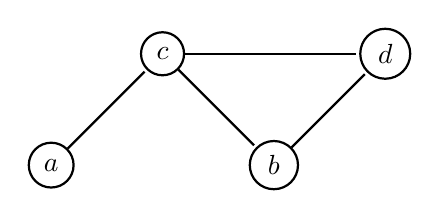
\begin{tikzpicture}[-,>=stealth,shorten >=1pt,auto,node distance=2cm, thick,main node/.style={scale=0.9,circle,draw,font=\sffamily\normalsize}]

            \node[circle, draw]  (1) []{$a$};
            \node[circle, draw]  (2) [above right of = 1]{$c$};
            \node[circle, draw]  (3) [below right of = 2]{$b$};
            \node[circle, draw]  (4) [above right of = 3]{$d$};

            % \path[every node/.style={font=\sffamily\small}]

            \draw[-] (1) to (2);
            \draw[-] (2) to (3);
            \draw[-] (2) to (4);
            \draw[-] (3) to (4);

            ;
        \end{tikzpicture}
    \end{figure}

    and the following edge orientation $\phi$:

    \begin{center}
        \begin{tabular}{c|c c c c} 
            $e$ & $ac$ & $bc$ & $bd$ & $cd$ \\
            \hline
            $\phi(e)$ & $c$ & $c$ & $b$ & $d$
        \end{tabular}
    \end{center}

    we get the following directed graph:

    \begin{figure}[H]
        \centering
        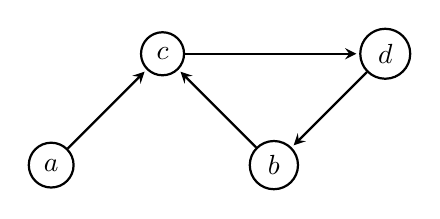
\begin{tikzpicture}[-,>=stealth,shorten >=1pt,auto,node distance=2cm, thick,main node/.style={scale=0.9,circle,draw,font=\sffamily\normalsize}]

            \node[circle, draw]  (1) []{$a$};
            \node[circle, draw]  (2) [above right of = 1]{$c$};
            \node[circle, draw]  (3) [below right of = 2]{$b$};
            \node[circle, draw]  (4) [above right of = 3]{$d$};

            % \path[every node/.style={font=\sffamily\small}]

            \draw[->] (1) to (2);
            \draw[->] (3) to (2);
            \draw[->] (2) to (4);
            \draw[->] (4) to (3);

            ;
        \end{tikzpicture}
        \label{oriented_graph}
    \end{figure}

    We observe that every graph has $2^{\abs{E(G)}}$ possible orientation. We denote with $\deg_{\phi}(v)$ the in-degree of a vertex $v$ over an orientation $\phi$, while $\Delta_\phi$ denotes the maximum degree under the orientation.
    \[\Delta_\phi = \max_{v \in V(G)} \deg_\phi(v)\]

    We observe that, similarly to the Handshaking Lemma, we have that:
    \[\sum_{v \in V(G)} \deg_\phi(v) = \abs{E(G)}\]

    After analyzing all the details and relations, Charikar came up with the following $\frac{1}{2}$-approximation.

    \begin{algorithm}[H]
        \caption{Charikar's $\frac{1}{2}$-approximation for DS}
        \textbf{Input:} an undirected graph $G$

        \textbf{Output:} a subset of vertices
        \begin{algorithmic}[1]
            \Function{$\frac{1}{2}$-approx-ds}{$G$}
                \State $S_0 \gets V(G)$
                \For{$i \in [n]$}
                    \State Find $v_i \in \argmin\limits_{v \in S_{i-1}} \deg_{G[S_{i-1}]}(v)$
                    \State $S_i \gets S_{i-1} - \{v\}$
                \EndFor
                \State Return $S \in \argmax_{i \in [n]} \rho(S_i)$
            \EndFunction
        \end{algorithmic}
    \end{algorithm}

    \begin{framedthm}[label={charikal}]{}
        Given a graph $G$, let $S^*$ be an optimal solution to $\mathrm{DS}(G)$. Given the output $S$ of \textsc{$\frac{1}{2}$-approx-ds}$(G)$, it holds that $\abs{S} \geq \frac{1}{2} \abs{S^*}$. 
    \end{framedthm}

    \begin{proof}
        Since the orientation problem is the dual of the densest subgraph, by the weak duality theorem we expect any orientation to give an upper bound on the density. In fact, the following claim holds.

        \textbf{Claim 1:} for any orientation $\phi$ on $G$ it holds that:
        \[\max_{S' \subseteq V(G)} \rho(S') \leq \Delta_\phi\]

        \begin{proof}
            Since any orientation can be restricted to an orientation over any induced subgraph of $G$, we get that:
            \[\max_{S' \subseteq V(G)} \frac{\abs{E(G[S'])}}{\abs{S'}} = \max_{S' \subseteq V(G)} \frac{\abs{\sum_{v \in S'} \deg_{\phi, G[S']}}}{\abs{S'}} \leq \frac{\abs{\sum_{v \in S'} \Delta_\phi}}{\abs{S'}} = \Delta_\phi\]
        \end{proof}
        
        Let $S_0, \ldots, S_n$ and $v_1, \ldots, v_n$ respectively be the subsets and vertices defined inside \textsc{$\frac{1}{2}$-approx-ds}$(G)$. Consider the orientation $\phi$ on $G$ defined as follows: for each $i \in [n]$ and for each edge $e \in G[S_{i-1}]$, if $v_i \in e$ then $\phi(e) = v_i$. In other words, $\phi$ is the orientation on $G$ such that each edge incident to the vertex $v_i$ removed in the $i$-th iteration gets oriented towards $v_i$.

        \textbf{Claim 2:} for each $i \in [n]$ it holds that $\deg_\phi(v_i) \leq 2 \rho(S_{i-1})$

        \begin{proof}
            By construction, we have that $\deg_\phi(v_i) = \deg_{G[S_{i-1}]}(v_i)$. Then, by choice of $v_i$ inside the algorithm, we have that:
            \[\deg_{G[S_{i-1}]}(v_i) = \min_{v \in S_{i-1}} \deg_{G[S_{i-1}]}(v) \leq \avg_{v \in S_{i-1}} \deg_{G[S_{i-1}]}(v) = \frac{\sum_{v \in S_{i-1}} \deg_{G[S_{i-1}]}(v)}{\abs{S_{i-1}}}\]

            By the Handshaking lemma, we conclude that:
            \[\deg_{G[S_{i-1}]}(v_i) \leq \frac{\sum_{v \in S_{i-1}} \deg_{G[S_{i-1}]}(v)}{\abs{S_{i-1}}} = \frac{2 \abs{E(G[S_{i-1}])}}{\abs{S_{i-1}}}\]
        \end{proof}

        Through the two claims, we conclude that:
        \[\rho(S^*) \leq \Delta_\phi = \max_{i \in [n]} \deg_{\phi}(v_i) \leq \max_{i \in [n]} 2 \rho(S_{i-1}) = 2 \rho(S)\] 
    \end{proof}

    \section{Approximation and runtime trade-offs}

    We showed how Charikar came up with an exact solution to the DS problem that runs in $O(n^9)$ and a $\frac{1}{2}$-approximation that is way faster. However, the number of iterations this approximation are still too many: we're iterating over $n$ nodes and each iteration requires $O(n+m)$ steps, making the total cost $O(n(n+m))$. For real-life purposes, this runtime is still too much -- for instance, Google could never use such algorithm to detect spam-networks since the underlying graph contains more than $10^{30}$ nodes. What if we modify the algorithm in order to make it remove a all the nodes of minimum degree instead of a single node at a time?

    \begin{algorithm}[H]
        \caption{Charikar's $\frac{1}{2}$-approximation for DS (2nd version)}
        \textbf{Input:} an undirected graph $G$

        \textbf{Output:} a subset of vertices
        \begin{algorithmic}[1]
            \Function{$\frac{1}{2}$-approx-ds}{$G$}
                \State $S_0 \gets V(G)$
                \For{$i \in [n]$}
                    \State Find $A_i = \{v \in S_{i-1} \mid \deg_{G[S_{i-1}]} (v) = \min_{u \in S_{i-1}} \deg_{G[S_{i-1}]}(u)\}$
                    \State $S_i \gets S_{i-1} - A_i$
                \EndFor
                \State Return $S \in \argmax_{i \in [n]} \rho(S_i)$
            \EndFunction
        \end{algorithmic}
    \end{algorithm}

    Even though this second version works better on average, there are still some instances for which it strictly requires almost $n$ iterations. For instance, consider the three graphs in the figure below. For the first graph, the new version requires only one iteration since every vertex has the same degree. For the second graph, it requires $\frac{n}{2}$ iterations, while the third graph requires $n-2$ iterations. 

    \begin{figure}[H]
        \centering
        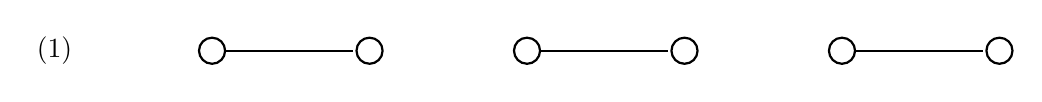
\begin{tikzpicture}[-,>=stealth,shorten >=1pt,auto,node distance=2cm, thick,main node/.style={scale=0.9,circle,draw,font=\sffamily\normalsize}]

            \node[circle, draw]  (1) []{};
            \node[circle, draw]  (2) [right of = 1]{};
            \node[circle, draw]  (3) [right of = 2]{};
            \node[circle, draw]  (4) [right of = 3]{};
            \node[circle, draw]  (5) [right of = 4]{};
            \node[circle, draw]  (6) [right of = 5]{};

            \node[]  (x) [left of = 1]{$(1)$};

            \path[every node/.style={font=\sffamily\small}]
                (1) edge (2)
                (3) edge (4)
                (5) edge (6)
            ;
        \end{tikzpicture}
        
        \qquad
        
        \qquad

        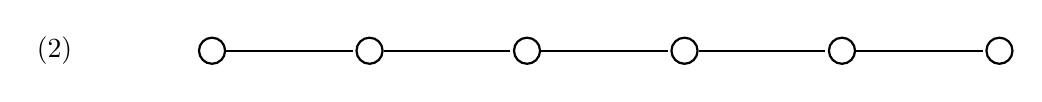
\begin{tikzpicture}[-,>=stealth,shorten >=1pt,auto,node distance=2cm, thick,main node/.style={scale=0.9,circle,draw,font=\sffamily\normalsize}]

            \node[circle, draw]  (1) []{};
            \node[circle, draw]  (2) [right of = 1]{};
            \node[circle, draw]  (3) [right of = 2]{};
            \node[circle, draw]  (4) [right of = 3]{};
            \node[circle, draw]  (5) [right of = 4]{};
            \node[circle, draw]  (6) [right of = 5]{};

            \node[]  (x) [left of = 1]{$(2)$};

            \path[every node/.style={font=\sffamily\small}]
                (1) edge (2)
                (2) edge (3)
                (3) edge (4)
                (4) edge (5)
                (5) edge (6)
            ;
        \end{tikzpicture}

        \qquad
        
        \qquad

        \begin{tikzpicture}[-,>=stealth,shorten >=1pt,auto,node distance=2cm, thick,main node/.style={scale=0.9,circle,draw,font=\sffamily\normalsize}]

            \node[circle, draw]  (1) []{};
            \node[circle, draw]  (2) [right of = 1]{};
            \node[circle, draw]  (3) [right of = 2]{};
            \node[circle, draw]  (4) [right of = 3]{};
            \node[circle, draw]  (5) [right of = 4]{};
            \node[]  (6) [right of = 5]{};
            \node[circle, draw]  (7) [above of = 6, yshift=-30]{};
            \node[circle, draw]  (8) [below of = 6, yshift=30]{};

            \node[]  (x) [left of = 1]{$(3)$};

            \path[every node/.style={font=\sffamily\small}]
                (1) edge (2)
                (2) edge (3)
                (3) edge (4)
                (4) edge (5)
                (5) edge (7)
                (5) edge (8)
                (7) edge (8)
            ;
        \end{tikzpicture}
    \end{figure}
    
    We observe that the proof of Charikar's doesn't require the selected vertices to be the ones with minimum degree: we require the vertices to be just below the average degree.

    \begin{algorithm}[H]
        \caption{Charikar's $\frac{1}{2}$-approximation for DS (3nd version)}
        \textbf{Input:} an undirected graph $G$

        \textbf{Output:} a subset of vertices
        \begin{algorithmic}[1]
            \Function{$\frac{1}{2}$-approx-ds}{$G$}
                \State $S_0 \gets V(G)$
                \For{$i \in [n]$}
                    \State Find $A_i = \{v \in S_{i-1} \mid \deg_{G[S_{i-1}]} (v) \leq \avg_{u \in S_{i-1}} \deg_{G[S_{i-1}]}(u)\}$
                    \State $S_i \gets S_{i-1} - A_i$
                \EndFor
                \State Return $S \in \argmax_{i \in [n]} \rho(S_i)$
            \EndFunction
        \end{algorithmic}
    \end{algorithm}

    We observe however, that this constraint is still \curlyquotes{too strict}: the third graph now requires 2 iterations, while the second graph still requires $\frac{n}{2}$ iterations since only the endpoints are below the average degree (which has value $\frac{10}{6} = 1.\overline{6}$). To fix this, we can make the boundary more flexible by adding a small bias factor of $(1+\varepsilon)$ to the selection criteria, where $\varepsilon > 0$. This solutions was proposed by \textcite{bahmani}, obtaining a solid upper bound on the number of iterations, with a small loss on the approximation rate. With this final version, we observe that even a small value such as $\varepsilon = 0.4$ is sufficient to make the algorithm run in 1 iteration even for the second case.

    \begin{algorithm}[H]
        \caption{$\frac{1}{2(1+\varepsilon)}$-approximation for DS}
        \textbf{Input:} an undirected graph $G$

        \textbf{Output:} a subset of vertices
        \begin{algorithmic}[1]
            \Function{$\frac{1}{2(1+\varepsilon)}$-approx-ds}{$G$}
                \State $S_0 \gets V(G)$
                \For{$i \in [n]$}
                    \State Find $A_i = \{v \in S_{i-1} \mid \deg_{G[S_{i-1}]} (v) \leq (1+\varepsilon)\avg_{u \in S_{i-1}} \deg_{G[S_{i-1}]}(u)\}$
                    \State $S_i \gets S_{i-1} - A_i$
                \EndFor
                \State Return $S \in \argmax_{i \in [n]} \rho(S_i)$
            \EndFunction
        \end{algorithmic}
    \end{algorithm}

    \begin{framedthm}[]{}
        Given a graph $G$, let $S^*$ be an optimal solution to $\mathrm{DS}(G)$. Given the output $S$ of \textsc{$\frac{1}{2(1+\varepsilon)}$-approx-ds}$(G)$, for all $\varepsilon > 0$  it holds that $\abs{S} \geq \frac{1}{2(1+\varepsilon)} \abs{S^*}$. Moreover, the algorithm \textsc{$\frac{1}{2(1+\varepsilon)}$-approx-ds} does at most $O(\log_{1+\varepsilon} n)$ iterations.
    \end{framedthm}

    \begin{proof}
        Let $S^*$ be the optimal solution. If $\rho(S^*) = 0$ then $E(G) = \varepsilon$, so any solution is optimal. Suppose now that $\rho(S^*) > 0$. Then, $E(G) \neq \varepsilon$, implying that $\abs{S^*} \geq 2$. This observation allows us to claim the following.

        \textbf{Claim}: for all $v \in S^*$ it holds that $\rho(S^*) \leq \deg_{S^*}(v)$.

        \begin{proof}[Proof of the claim.]
            Fix a vertex $v \in S^*$. By optimality of $S^*$, we know that $\rho(S^*) \geq \rho(S^* - \{v\})$. Moreover, we observe that:
            \[\rho(S^*-\{v\}) = \frac{\abs{E(G[S^*-\{v\}])}}{\abs{S^*-\{v\}}} = \frac{\abs{E(G[S^*])} - \deg_{S^*}(v)}{\abs{S^*}-1}\]

            Hence, we get that:
            \[\rho(S^*) \geq \rho(S^* - \{v\}) \implies \frac{\abs{E(G[S^*])}}{\abs{S^*}} \geq \frac{\abs{E(G[S^*])} - \deg_{S^*}(v)}{\abs{S^*}-1}\]

            The claim follows by solving the inequality.
        \end{proof}

        We observe that by construction of the algorithm at least one node is removed in each iteration since at least the vertex with minimum degree will be selected:
        \[\min_{v \in S_{i-1}} \deg_{G[S_{i-1}]}(v) \leq \avg_{v \in S_{i-1}} \deg_{G[S_{i-1}]}(v) \leq (1+\varepsilon)\avg_{v \in S_{i-1}} \deg_{G[S_{i-1}]}(v)\]

        Hence, the algorithm will eventually select a vertex of $S^*$. Let $i$ be the first iterations such that $A_i \cap S^* \neq \varepsilon$. Moreover, since $i$ is the smallest iteration with such property, it must hold that $S^* \subseteq S_{i-1}$. Hence, given any vertex $v_i \in A_i \cap S^*$ it holds that:
        \[\rho(S^*) \leq \deg_{S^*} (v) \leq \deg_{S_{i-1}}(v) \leq (1+\varepsilon
        ) \avg_{v \in S_{i-1}} \deg_{G[S_{i-1}]}(v) = 2(1+\varepsilon) \rho(S_i)\]

        Thus, we conclude that:
        \[\rho(S_{i-1}) \geq \frac{1}{2(1+\varepsilon)} \rho(S^*)\]

        meaning that the solution $S$ returned by algorithm will be at least as good as a $\frac{1}{2(1+\varepsilon)}$-approximation.
        \[S \in \argmax_{j\in [n]} \rho(S_j) \geq \rho(S_{i-1}) \geq \frac{1}{2(1+\varepsilon)} \rho(S^*)\]

        Consider now a generic iteration $k \in [n]$. We observe that:
        \[\begin{split}
            2\abs{E(G[S_k])} &= \sum_{v \in S_k} \deg_{G[S_k]}(v) \\
            &= \sum_{v \in A_k} \deg_{G[S_k]}(v) + \sum_{v \in S_k-A_k} \deg_{G[S_k]}(v) \\
            &\geq \sum_{v \in S_k-A_k} \deg_{G[S_k]}(v) \\
            &> \sum_{v \in S_k-A_k} (1+\varepsilon) \avg_{u \in S_k} \deg_{G[S_k]}(u) \\
            &= (\abs{S_k}-\abs{A_k})(1+\varepsilon) \avg_{u \in S_k} \deg_{G[S_k]}(u) \\
            &= \abs{S_{k+1}}(1+\varepsilon) \frac{2 \abs{E(G[S_k])}}{\abs{S_k}}
        \end{split}\]

        Thus, we get that:
        \[2\abs{E(G[S_k])} > \abs{S_{k+1}}(1+\varepsilon) \frac{2 \abs{E(G[S_k])}}{\abs{S_k}}\implies 1 > \frac{\abs{S_{k+1}}}{\abs{S_k}} (1+\varepsilon) \implies \abs{S_{k+1}} < \frac{\abs{S_k}}{1+\varepsilon}\]

        Let $i^*$ be the last iteration of the algorithm. Since $\abs{S_0} = n$ and since $i^*$ is reached when $\abs{S_{i^*}} = 1$, we get that:
        \[\abs{S_{i^*}} < \frac{n}{(1+\varepsilon)^{i^*}} \implies 1 < \frac{n}{(1+\varepsilon)^{i^*}} \implies i^* \leq \log_{1+\varepsilon} n\]
    \end{proof}

    \section{Approximations through Semidefinite programming}

    In \Cref{max_cut}, we briefly mentioned how the best known approximation ratio for the Max-Cut problem is around $0.878$. After developing all the standard tools for approximations through linear programs, we're finally ready to discuss such ratio. First, let's take a step back to were we started. We gave a $\frac{1}{2}$-approximation for Max-Cut that doesn't even care about the structure of the graph itself: the algorithm simply flips a coin and decides if the corresponding vertex has to be added or not.

    Using the new tools that we know, we start by formulating an integer program that exactly models the Max-Cut problem. For each edge $\{i,j\}$ we define a variable $y_{i,j}$, while for each vertex $v$ we define the variable $x_v$.
    
    \begin{figure}[H]
        \centering 
        \[\begin{array}{ccl}
            \qquad\qquad\quad
            & \displaystyle \max \; \sum_{\{i,j\} \in E(G)} y_{i,j} \\\\
            & y_{i,j} \leq x_i + x_j & \forall \{i,j\} \in E(G) \\
            & y_{i,j} \leq 2 - (x_i + x_j) & \forall \{i,j\} \in E(G) \\
            & x \in \{0,1\}^{n} \\
            & y \in \{0,1\}^{m} \\
        \end{array}\]
        \caption{Integer program for the Max-Cut problem.}
    \end{figure}

    However, we observe that in the LP relaxation of such program the optimal solution will always set every single vertex variable $x_v$ to $\frac{1}{2}$ and every edge variable $y_{i,j}$ to $1$. In other words, the optimal solution to the LP relaxation gives us no information at all! In fact, this is the reason why $\frac{1}{2}$-approximation can just flip coins for every vertex without considering the structure of the graph. But how good can this relaxation get? We already know that our algorithm gives implies that $\mathrm{IG}_{\mathrm{MC}} \leq 2$. Moreover, it can be proven that for any $n \in \N$ the gap of $K_n$ is at least $2-\varepsilon$, for some $\varepsilon > 0$, concluding that $\mathrm{IG}_{\mathrm{MC}} = 2$ holds for this program.
    
    Since the exact LP relaxation always gives a trivial solution with a gap of $2$, researchers tried for many years to improve the gap by considering variants of the program, introducing constraints that may improve the gap. However, each try failed.
    
    \begin{figure}[H]
        \centering 
        \[\begin{array}{ccl}
            \qquad\qquad\quad
            & \displaystyle \max \; \sum_{\{i,j\} \in E(G)} y_{i,j} \\\\
            & y_{i,j} \leq x_i + x_j & \forall \{i,j\} \in E(G) \\
            & y_{i,j} \leq 2 - (x_i + x_j) & \forall \{i,j\} \in E(G) \\
            & y_{i,j} + y_{j,k} + y_{k,i} \leq 2 & \forall \{i,j,k\} \in \binom{V(G)}{3} \text{ s.t. } i \sim j \sim k \\
            & x \in \{0,1\}^{n} \\
            & y \in \{0,1\}^{m} \\
        \end{array}\]
        \caption{Variant of the IP with an additional \curlyquotes{triangle constraint}, which forces the solution to have at most 2 edges for each $K_3$ inside the graph.}
    \end{figure}

    In the '90s, many results proved that even by adding a polynomial amount of constraints to the original problem, each with a constant number of variables, while keeping it a Max-Cut relaxation, the integrality gap is still lower bounded by $2-\varepsilon$ for any $\varepsilon > 0$, making researchers believe that no improvement could be achieved. 
    
    Surprisingly, \textcite{goemans_williamson} proved in a ground breaking result that this gap can indeed be improved, but only by completely changing the approach: instead of using an integer linear program, they modeled the Max-Cut problem through a \textbf{Quadratic Program (QP)}.

    \begin{figure}[H]
        \centering 
        \[\begin{array}{ccl}
            \qquad\qquad\quad
            & \displaystyle \max \; \frac{1}{2}x^TQx+c^Tx\\\\
            & Ax \leq b \\
            & x \in V \\
        \end{array}\]
        \caption{Standard form of a quadratic program.}
    \end{figure}

    The QP that exactly models the Max-Cut is very similar to the IP that models it, with the exception of edge constraints being \curlyquotes{implicit} in the objective function.

    \begin{figure}[H]
        \centering 
        \[\begin{array}{ccl}
            \qquad\qquad\quad
            & \displaystyle \max \; \sum_{\{i,j\} \in E(G)} \frac{1-x_ix_j}{2}\\\\
            & x \in \{1,-1\}^n \\
        \end{array}\]
        \caption{Quadratic program for the Max-Cut problem.}
    \end{figure}

    We observe that for any edge $\{i,j\}$ we have that:
    \[ \frac{1-x_ix_j}{2} = \soe{ll}{
        0 & \text{if } x_i = x_j \\
        1 & \text{if } x_i \neq x_j \\
    }\]

    Nonetheless, solving quadratic programs is also $\mathsf{NP}$-Hard. However, the genius idea of Goemans and Williamson involved \textit{casting} such quadratic program into a \textbf{Semidefinite Program (SDP)}. 

    \begin{figure}[H]
        \centering 
        \[\begin{array}{ccl}
            \qquad\qquad\quad
            & \displaystyle \max \; \sum_{i,j \in [n]} c_{i,j} \abk{v_i, v_j}\\\\
            & \displaystyle \max \; \sum_{i,j \in [n]} a_{i,j,k} \abk{v_i, v_j} \leq b_k& \forall k \in [n] \\
            & v_i \in \R^n & \forall i \in [n] \\
        \end{array}\]
        \caption{Standard form of a semidefinite program.}
    \end{figure}

    We observe that differently from linear and quadratic programs, SDPs work on \textit{vector variables}, where $\abk{v_i, v_j}$ denotes the dot product. Like LPs, SDPs can also be solved in polynomial time through an extension of the Ellipsoid method., making them a good tool for algorithm design. In particular, they are mostly used for \textit{computational geometry}.
    
    \begin{figure}[H]
        \centering 
        \[\begin{array}{ccl}
            \qquad\qquad\quad
            & \displaystyle \max \; \sum_{\{i,j\} \in E(G)} \frac{1-\abk{v_i,v_j}}{2}\\\\
            & \abk{v_i, v_i} = 1 & \forall i \in [n]\\\\
            & v_i \in \R^n & \forall i \in [n] \\
        \end{array}\]
        \caption{Goemans and Williamson's SDP relaxation for the Max-Cut problem.}
    \end{figure}

    The correctness of this relaxation comes in a pretty natural way. Let $\overline{x}$ be a feasible solution to the QP. If we map each component $\overline{x}_i$ with the vector $v_i = \smat{\overline{x}_i & 0 & \ldots & 0}^T$, we observe that:
    \[\abk{v_i, v_j} = \sum_{k \in [n]} v_{k,i} v_{k,j} = \overline{x}_i \overline{x}_j\]

    Moreover, the constraint $\abk{v_i, v_i} = 1$ is always satisfied:
    \[\abk{v_i, v_i} = \sum_{k \in [n]} v_{k,i}^2 = \overline{x}_i^2 = 1\]

    This concludes that $\mathrm{SDP}_{\mathrm{MC}}^* \geq \mathrm{QP}^* = \mathrm{OPT}_{\mathrm{MC}}$. The algorithm proposed by the two authors, however, is not so natural. In fact, it looks pretty much like \textit{black magic}.

    \begin{algorithm}[H]
        \caption{GW $0.878$-approximation for MC}
        \textbf{Input:} an undirected graph $G$

        \textbf{Output:} a cut of $G$
        \begin{algorithmic}[1]
            \Function{$0.878$-approx-mc}{$G$}
                \State $\{v_1, \ldots, v_n\} \gets \mathrm{SDP}_{\mathrm{MC}}(G)$
                \State $S_n \gets \{x \in \R^n \mid \norm{x} = 1\}$
                \Comment $S_n$ is the $n$-dimensional hypersphere
                \State Sample a uniform-at-random vector $y$ from $S_n$
                \State $S \gets \{i \mid \abk{v_i, y} \geq 0 \}$
                \State Return $(S, \overline{S})$
            \EndFunction
        \end{algorithmic}
    \end{algorithm}

    \begin{framedthm}{}
        Given a graph $G$, let $(S^*, \overline{S^*})$ be an optimal solution to $\mathrm{MC}(G)$. Given the output $(S, \overline{S})$ of \textsc{$0.878$-approx-mc}$(G)$, it holds that 
        \[\Exp[\abs{\mathrm{cut}(S, \overline{S})}] \geq \alpha_{\mathrm{GW}} \cdot \abs{\mathrm{cut}(S^*, \overline{S^*})}\]

        where:
        \[\alpha_{\mathrm{GW}} = \frac{2}{\pi} \min_{x \in (-1,1)} \frac{\arccos(x)}{\pi} = 0.878\ldots\]
    \end{framedthm}

    \begin{proof}[Proof. (Sketch)]
        A formal proof of this claim would require advanced analytical arguments that are out of the scope of this course. We give an informal intuition behind how and why the algorithm works by focusing on the 2D case. First, we observe that the dot product between two vectors $u,w$ can be geometrically described as:
        \[\abk{u,w} = \norm{u} \cdot \norm{w} \cdot \cos(\theta_{u,w})\]

        where $\theta_{u,w}$ is the angle between the two vectors. Since each $v_1, \ldots, v_n$ has to satisfy the constraint $\abk{v_i, v_i} = 1$, we know that:
        \[1 = \abk{v_i, v_i} = \norm{v_i}^2 \implies 1 = \norm{v_i}\]

        Hence, since the vector $y$ is sampled from $S_n$, we get that $\abk{v_i,y} = \cos(\theta_{v_i, y})$. We also observe that for any angle $\theta$ it holds that:
        \[\cos(\theta) \geq 0 \iff 2k\pi - \frac{\pi}{2} \leq \theta \leq 2k\pi + \frac{\pi}{2}\]

        Geometrically, this describes the fact that the two vertices are \textit{close enough} (see \Cref{gw_1}). In other words, the set $S$ contains vectors that are similar to each other (up to some degree of freedom). This vector-comparison metric is often used in Machine Learning. 

        \textbf{Claim 1}: $\displaystyle \Pr[\{i,j\} \in \mathrm{cut}(S, \overline{S})] = \frac{\theta_{v_i, v_j}}{\pi}$

        \begin{proof}[Proof of Claim 1.]
            For each $k \in [n]$, let $H_k$ be the $1$-dimensional hyperplane passing through the origin and perpendicular to $v_k$. This hyperplane splits $S_2$ in half: one half contains all the vectors $x$ such that $\cos(\theta_{v_k, x}) \geq 0$, while all the others lie on the other half. 

            Consider now the two hyperplanes $H_i, H_j$ and \Cref{gw_2}. We notice that two hyperplanes induce a another split of $S_2$ into four subspaces:
            \begin{enumerate}
                \item The green sector contains all the vectors $x$ such that $\cos(\theta_{v_i, x}) \geq 0$ and $\cos(\theta_{v_j, x}) \geq 0$
                \item The blue sector contains all the vectors $x$ such that $\cos(\theta_{v_i, x}) \geq 0$ and $\cos(\theta_{v_j, x}) < 0$
                \item The yellow sector contains all the vectors $x$ such that $\cos(\theta_{v_i, x}) < 0$ and $\cos(\theta_{v_j, x}) \geq 0$
                \item The white sector contains all the vectors $x$ such that $\cos(\theta_{v_i, x}) < 0$ and $\cos(\theta_{v_j, x}) < 0$
            \end{enumerate}

            We also observe that the angle describing the yellow and blue sectors is exactly equal to $\theta_{v_i, v_j}$. Hence, the portion of the sphere for both sectors is given by $\frac{\theta_{v_i, v_j}}{2\pi}$, implying that:
            \[\begin{split}
                \Pr[\{i,j\} \in \mathrm{cut}(S, \overline{S})] &= \Pr[i \in S, j \notin S \lor i \notin S, j \in S] \\
                &= \Pr[i \in S, j \notin S] + \Pr[i \notin S, j \in S] \\
                &= \frac{\theta_{v_i, v_j}}{2\pi} + \frac{\theta_{v_i, v_j}}{2\pi} \\
            \end{split}\]
        \end{proof}

        Through Claim 1, we get that:
        \[\begin{split}
            \Exp[\abs{\mathrm{cut}(S, \overline{S})}] &= \sum_{\{i,j\} \in E(G)} \Pr[\{i,j\} \in \mathrm{cut}(S, \overline{S})] \\
            &= \sum_{\{i,j\} \in E(G)} \frac{\theta_{v_i, v_j}}{\pi} \\
            &= \sum_{\{i,j\} \in E(G)} \frac{\arccos(\abk{v_i,v_j})}{\pi}
        \end{split}\]

        \textbf{Claim 2}: if $\alpha \in \R$ is a value such that $\displaystyle \alpha \leq \frac{2}{\pi} \frac{\arccos(x)}{1-x}$ for all $x \in (-1,1)$ then
        \[\Exp[\abs{\mathrm{cut}(S, \overline{S})}] \geq \alpha \mathrm{SPD}_{MC}^*(G)\]

        \begin{proof}[Proof of Claim 2.]
            Through some algebraic manipulation we get that:
            \[\frac{\arccos(x)}{\pi} \geq \alpha \rbk{\frac{1-x}{2}}\]

            Hence, since $-1 \leq \abk{v_i,v_j} \leq 1$, it holds that:
            \[\Exp[\abs{\mathrm{cut}(S, \overline{S})}] \geq \sum_{\{i,j\} \in E(G)} \frac{\arccos(\abk{v_i,v_j})}{\pi} \geq \alpha \sum_{\{i,j\} \in E(G)} \rbk{\frac{1-\abk{v_i,v_j}}{2}} = \alpha \mathrm{SPD}_{MC}^*(G)\]
        \end{proof}

        In order to satisfy Claim 2, it's sufficient to consider the value $\alpha_{\mathrm{GW}}$ defined as:
        \[\alpha_{\mathrm{GW}} = \frac{2}{\pi} \min_{x \in (-1,1)} \frac{\arccos(x)}{\pi} = 0.878\]

        Moreover, since the SDP is a relaxation of the QP, we get that:
        \[\Exp[\abs{\mathrm{cut}(S, \overline{S})}] \geq \alpha_{\mathrm{GW}} \mathrm{SPD}_{MC}^*(G) \geq \alpha_{\mathrm{GW}} \mathrm{QP}_{MC}^*(G)\]
    \end{proof}

    \begin{figure}[H]
        \centering
        \includegraphics[scale=0.65]{images/gw_1.png}
        \caption{If $y$ falls in the blue sector then $\cos(\theta_{v_i, y}) \geq 0$, hence $i \in S$.}
        \label{gw_1}
    \end{figure}

    \begin{figure}[H]
        \centering
        \includegraphics[scale=0.65]{images/gw_2.png}
        \caption{Partition of $S_2$ into the four subspaces induced by $H_i, H_j$. }
        \label{gw_2}
    \end{figure}

    We observe that the approximation ratio $\alpha_\mathrm{GW}$ for the MC problem is actually \textit{tight}. In fact, it can be proven that $\mathrm{IG}_{\mathrm{GW}}^{\mathrm{SDP}} = \alpha_\mathrm{GW}$: the above proof of the algorithm implicitly gives the lower bound, while the upper bound is given by the graph $C_n$. For instance, consider the following $C_5$ graph.

    \begin{figure}[H]
        \centering
        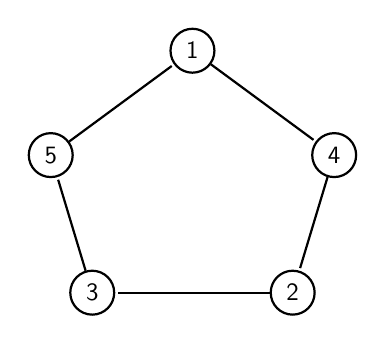
\begin{tikzpicture}[-,>=stealth,shorten >=1pt,auto,node distance=2cm,thick,main node/.style={scale=0.9,circle,draw,font=\sffamily\normalsize}]
            \node[] (x) {};
            \node[main node] (1) [above of = x] {1};
            \node[main node] (2) [right of = x, yshift=15]{4};
            \node[main node] (3) [below right of = x]{2};
            \node[main node] (4) [below left of = x]{3};
            \node[main node] (5) [left of = x, yshift=15]{5};

            \path[every node/.style={font=\sffamily\small}]
                (1) edge (2)
                (2) edge (3)
                (3) edge (4)
                (4) edge (5)
                (5) edge (1)
                ;
        \end{tikzpicture}
        
        \caption{The graph $C_5$ giving the lower bound for $\mathrm{IG}_{\mathrm{MC}}^{\mathrm{SDP}}$.}
    \end{figure}

    We observe that the order of the indices labeling such vertices is not arbitrary, but carefully chosen in order to make the following computations easier. First, we notice that the cut $(\{1,2\}, \{3,4,5\})$ is optimal for this graph, meaning that $\mathrm{OPT}_{\mathrm{MC}}(C_5) = 4$. We'll now construct a feasible solution to the SDP program in order to get a lower bound on $\mathrm{SDP}^*$. For every $j \in [n]$, we set:
    \[v_j = \smat{\cos \rbk{\frac{2j\pi}{5}} & \sin \rbk{\frac{2j\pi}{5}} & 0 & 0 & 0}\]

    It's easy to see that every vertex satisfies the constraint of the SDP:
    \[\abk{v_j, v_j} = \cos^2 \rbk{\frac{2j\pi}{5}} + \sin^2 \rbk{\frac{2j\pi}{5}} = 1\]

    Moreover, using the same reasoning as the previous proof we know that:
    \[\sum_{\{i,j\} \in E(C_5)} \frac{1-\abk{v_i, v_j}}{2} = \sum_{\{i,j\} \in E(C_5)} \frac{1-\cos(\theta_{v_i,v_j})}{2}\]

    Now, we observe that the angle between each pair $v_i,v_j$ such that $\{i,j\} \in E(C_5)$ is exactly $\frac{4\pi}{5}$ (see \Cref{gw_3}). Hence, we get that:
    \[\sum_{\{i,j\} \in E(C_5)} \frac{1-\abk{v_i, v_j}}{2} = \sum_{\{i,j\} \in E(C_5)} \frac{1-\cos\rbk{\frac{4\pi}{5}}}{2} = \frac{5(1-\cos\rbk{\frac{4\pi}{5}})}{2}\]

    Thus, the integrality gap for $C_5$ corresponds to:
    \[\mathrm{IG}_{\mathrm{MC}}^{\mathrm{SDP}} = \frac{4}{\dfrac{5(1-\cos\rbk{\frac{4\pi}{5}})}{2}} = 0.884\ldots\]

    concluding that $0.878 \approx \alpha_{\mathrm{GW}} \leq \mathrm{IG}_{\mathrm{MC}}^{\mathrm{SDP}} \leq \mathrm{IG}_{\mathrm{MC}}^{\mathrm{SDP}}(C_5) \approx 0.884$.

    \begin{figure}[H]
        \centering
        \includegraphics[scale=0.65]{images/gw_3.png}
        
        \caption{The vectors $v_1,\ldots, v_5$ actually describe the 5 roots of unity. For $C_n$, the argument is generalized to the $n$ roots of unity.}
    \end{figure}

    \begin{framedthm}{Integrality gap of MC with SDP}
        $\mathrm{IG}_{\mathrm{MC}}^{\mathrm{SDP}} = \alpha_\mathrm{GW} \approx 0.878$
    \end{framedthm}

    Hence, we conclude that Goemans and Williamson's algorithm is the best rounding algorithm that can be achieved through SDPs. Moreover, researchers believe that this approximation ratio is the best that can be achieved for the MC problem over all techniques. In particular, the main tool of reasoning behind this result is the \textbf{Unique Games Conjecture}, which will be discussed in the following section.
    
    \section{The Unique Games Conjecture}
    
    Before diving into the conjecture, we have to define the concept of \textbf{Unique Label Cover}, first defined by \textcite{khot}. We're given a bipartite graph with bipartition $(A,B)$ and a set of $k$ labels (also called \textit{colors}). Each edge $e \in E(G)$ has a permutation $\pi_{e} : [k] \to [k]$. An ULC is an assignment $\phi$ that labels each vertex with a color. An edge $\{a,b\}$ of the graph is said to be \textit{satisfied} by $\phi$ if the color $\phi(a)$ gets permuted into the color $\phi(b)$ by the permutation $\pi_{\{a,b\}}$.

    \begin{frameddefn}{Unique Label Cover}
        Let $G$ be a bipartite graph with bipartition $(A,B)$. Given a value $k \in \N$ and a permutation $\pi_e : [k] \to [k]$ for each $e \in E(G)$, an \textbf{unique label cover} of $G$ is an assignment $\phi : A \cup B \to [k]$ defining the set $S_\phi$ of satisfied edges:
        \[S_\phi = \{\{a,b\} \in E(G) \mid a \in A, b \in B, \pi_{\{a,b\}}(\phi(a)) = \phi(b)\}\]
    \end{frameddefn}

    \begin{figure}[H]
        \centering
        \includegraphics[scale=1.2]{images/ucl_3.png}

        \caption{(a) and (c) are two instances of the ULC problem with 2 colors. In (b) is a solution to (a) that satisfies all the edges, while (d) is a solution to (c) with an unsatisfied edge.}
    \end{figure}

    We observe that the ULC instances are \textit{strongly constrained} in the sense that the color of a vertex uniquely defines the colors of its neighbors and, by propagation, of its entire connected component. Thus, if the input instance admits a valid assignment, then such an assignment can be found efficiently by iterating over all colors of a single node. In particular, this implies that the problem of deciding if a given instance admits a satisfying assignment can be solved in polynomial time. 

    The \textit{value} of a ULC instance is the ratio of edges that are satisfiable by any assignment. For satisfiable instances, this value is 1 and is easy to find through the above procedure. On the other hand, it seems to be very difficult to determine the value of an unsatisfiable game, even approximately. Khot's \textbf{Unique Games Conjecture} formalizes this difficulty in terms of $\mathsf{NP}$-hardness.

    \begin{framedconj}{Unique Games Conjecture}
        It is conjectured that for each $\varepsilon > 0$ there is a value $k_\varepsilon$ for which it is $\mathsf{NP}$-Hard to determine if for an ULC problem with $k_\varepsilon$ labels one of the following holds:
        \begin{itemize}
            \item At most an $\varepsilon$-fraction of the edges are satisfied
            \item At least an $(1-\varepsilon)$-fraction of the edges are satisfied
        \end{itemize}
    \end{framedconj}

    Khot's conjecture has been proven to be intrinsically linked with \textbf{Constraint Satisfaction Problems (CSP)}, a particular subset of optimization problems. CSPs are defined in terms of a set of values $[q]$ and a set of \textit{$k$-ary} predicates $\mathcal{P}$ on $[q]$ -- the \textit{arity} of a predicate on $[q]$ is a function $f : [q]^k \to \{0,1\}$. An instance of a CSP is given by a set of variables $x_1, \ldots, x_n$ taking value over $[q]$ and a set of constraints, each taken from $\mathcal{P}$ and redefined over a subset of $k$ variables $x_{i_1}, \ldots, x_{i_k}$.

    \begin{frameddefn}{Constraint Satisfaction Problem (CSP)}
        Let $\mathcal{P}$ be a set of $k$-ary predicates defined on $[q]$, where $q,k \in \N$. An instance of a \textbf{Constraint Satisfaction Problem (CSP)} is a set of variables $X = \{x_1, \ldots, x_n\}$ and a set of constraints $C_1, \ldots, C_m$ such that $C_j = \abk{I_j, P_j}$, where $I_j \subseteq [n]$ and $P_j \in \mathcal{P}$. A constraint $C_j = \abk{I_j, P_j}$ is said to be satisfied by an assignment $\alpha : I_j \to \{0,1\}$ if $P_j\smat{x_{i_1} & \cdots & x_{i_k} \\ \alpha(x_{i_1}) & \cdots & \alpha(x_{i_k})}$ evaluates as true.
    \end{frameddefn}


    The goal of a CSP problem is to find an assignment maximizing the number of satisfied constraint. Lots of optimization problems, even those that we have already discussed, can be described in terms of CSP. 
    \begin{enumerate}
        \item The \textit{max-cut problem} can be described in terms of a CSP with value $q = 2$ and predicate set $\mathcal{P} = \{p(a,b)\}$ with arity 2, where $p(a,b) = $ \curlyquotes{$a \neq b$}. Given a graph $G$, for each node $x \in V(G)$ we define the variable $x_v$ and for each edge $\{u,v\} \in E(G)$ we define the constraint $p(x_u,x_v)$
        \item The \textit{max $k$-coloring problem} asks to find a $k$-coloring of a graph that maximizes the number of well-colored edges, that being the edges whose endpoints have different color. This problem can be described in terms of a CSP with value $q = k$ and predicate set $\mathcal{P} = \{p(a,b)\}$ with arity 2, where $p(a,b) = \curlyquotes{a \neq b}$. Given a graph $G$, for each node $x \in V(G)$ we define the variable $x_v$ and for each edge $\{u,v\} \in E(G)$ we define the constraint $p(x_u,x_v)$ -- this is basically a generalization of the max-cut problem.
        \item The \textit{max 3-sat problem} asks to find an assignment maximizing the number of clauses satisfied in a 3CNF formula. This problem can be described in terms of a CSP with value $q = 2$ and predicate set:
        \[\begin{split}
            \mathcal{P} = \{ &p_0(a,b,c) = \text{\curlyquotes{$a \lor b \lor c$}}, p_1(a,b,c) = \text{\curlyquotes{$a \lor b \lor \overline{c}$}}, \\
            & p_2(a,b,c) = \text{\curlyquotes{$a \lor \overline{b} \lor c$}}, p_3(a,b,c) = \text{\curlyquotes{$a \lor \overline{b} \lor \overline{c}$}}, \\
            & p_4(a,b,c) = \text{\curlyquotes{$\overline{a} \lor b \lor c$}}, p_5(a,b,c) = \text{\curlyquotes{$\overline{a} \lor b \lor \overline{c}$}}, \\
            & p_6(a,b,c) = \text{\curlyquotes{$\overline{a} \lor \overline{b} \lor c$}}, p_7(a,b,c) = \text{\curlyquotes{$\overline{a} \lor \overline{b} \lor \overline{c}$}}\}
        \end{split}\]

        For instance, given the formula $F = (\overline{x_1} \lor x_2 \lor x_7) \land (\overline{x_3} \lor \overline{x_4} \lor \overline{x_{10}})$ we define the constraints $p_4(x_1,x_2,x_7)$ and $p_7(x_3,x_4,x_{10})$
    \end{enumerate}

    \textcite{raghavendra} used CSPs to show that the connection between approximation algorithms, SDPs and the Unique Games Conjecture is as deep as possible. In fact, if the conjecture is proven to be true, Raghavendra's theorem directly implies that the SDP integrality gap of every problem describable through a CSP is the best possible approximation ratio. Many researchers believe the conjecture to be true, but none has yet proven it. Given a problem describable through a CSP $\mathcal{C}$, we denote with $\alpha(\mathcal{C})$ the best possible approximation ratio for $\mathcal{C}$, i.e. the minimum ratio such that the problem doesn't become $\mathsf{NP}$-Hard to approximate.
    
    \begin{framedthm}{Raghavendra's theorem}
        For every CSP $\mathcal{C}$ with values in $[q]$ and arity $k$, it holds that:
        \begin{itemize}
            \item There is an SDP with integrality gap of $\alpha(\mathcal{C})$ and a rounding algorithm that is an $\alpha(\mathcal{C})$-approximation of $\mathcal{C}$
            \item If the Unique Games Conjecture is true, it is $\mathsf{NP}$-Hard to approximate $\mathcal{C}$ with a ratio $\alpha(\mathcal{C})-\varepsilon$ for any $\varepsilon > 0$
        \end{itemize}
    \end{framedthm}

    \begin{proof}
        Omitted.
    \end{proof}

    As a direct corollary of Raghavendra's theorem, we get that the previously found approximation ratios for max-cut and vertex cover are the best possible ones. 

    \begin{framedcor}{}
        If the Unique Games Conjecture is true then $\mathrm{IG}_{\mathrm{MC}}^{\mathrm{SDP}} = \alpha(\mathrm{MC})$ and  $\mathrm{IG}_{\mathrm{VC}} = \alpha(\mathrm{VC})$
    \end{framedcor}
    
    \chapter{Metric geometry}

    \section{Metrics and isometrical embeddings}

    At this point, we have widely discussed the max-cut problem, showing that it is $\mathsf{NP}$-Hard and arguing that the Goemans-Williamson $0.878$-approximation is probably the best that can be achieved. Moreover, we also briefly mentioned that the min-cut problem can, instead, be solved in polynomial time through a reduction to the maximum flow problem, using the \textit{Max-flow/Min-cut theorem}.

    Now, we'll introduce a variant of the Min-cut problem: the \textit{Sparsest Cut} problem. Given a graph $G$, the \textbf{Sparsest Cut} problem asks to find a non-empty subset of vertices $S$ whose \textit{sparsity} $\psi(S)$ is minimized, where:
    \[\psi(S) = \frac{\abs{\mathrm{cut}(S,\overline{S})}}{\abs{S \times \overline{S}}} = \frac{\abs{\mathrm{cut}(S,\overline{S})}}{\abs{S} \cdot \abs{\overline{S}}}\]

    In other words, the goal is to partition a given graph into two large pieces while removing as few edges as possible. The sparsest cut problem plays an important role in theory of network flow, geometric embeddings and form a crucial component of divide-and-conquer approaches in applications such as packet routing, VLSI layout and clustering.

    A good tool of reasoning for the S-Cut problem is the \textbf{Erdős-Rényi Random Graph} \cite{random_graph}. Given two values $n,\mu$, where $n \in \N$ and $0 \leq \mu \leq 1$, the Erdős-Rényi graph, written as $G(n, \mu)$, is a graph with a fixed vertex set $V(G) = [n]$ and a probabilistic edge set, where each edge $e \in \binom{[n]}{2}$ has probability $\mu$ of being added to the edge set.
    \[\forall e \in \binom{[n]}{2} \;\; \Pr[e \in E(G)] = \mu\]

    By definition, this model represents a \curlyquotes{evenly sparse graph}. In fact, we observe that for each non-empty subset $S \subseteq V(G)$ it holds that:
    \[\Exp[\psi(S)] = \frac{\Exp{\abs{\mathrm{cut}(S, \overline{S})}}}{\abs{S} \cdot \abs{\overline{S}}} = \frac{\sum_{\{i,j\} \in S \times \overline{S}} \Pr[\{i,j\} \in \mathrm{cut}(S, \overline{S})]}{\abs{S} \cdot \abs{\overline{S}}} = \frac{\mu \cdot \abs{S} \cdot \abs{\overline{S}}}{\abs{S} \cdot \abs{\overline{S}}} = \mu\]

    For general graphs, we observe that for each non-empty subset $S \subseteq V(G)$ it holds that:
    \[0 \leq \abs{\mathrm{cut}(S, \overline{S})} \leq \abs{S} \cdot \abs{\overline{S}}\]

    implying that $0 \leq \psi(S) \leq 1$. In particular, we observe that $\psi(S) = 0$ holds when $S$ is disconnected from $\overline{S}$, while $\psi(S) = 1$ when $S$ is \curlyquotes{fully connected} to $\overline{S}$, meaning that every edge of $S$ is connected to every edge of $\overline{S}$.

    Considering the set $S^*$ inducing the minimal sparsity value $\psi(S^*)$, we have that $\psi(S^*) = 0$ when the whole graph $G$ is disconnected, while $\psi(S^*) = 1$ when $G$ is a complete graph, i.e. $G = K_n$.

    Not-so surprisingly, the Max-Cut problem can be reduced to the S-Cut problem, implying that the latter is also $\mathsf{NP}$-Hard. The problem can, however, be approximated through the \textit{Leighton-Rao algorithm}. This algorithm is based on LP relaxation and a series of reduction. In particular, the integrality gap of such algorithm is bounded by \textit{geometrical arguments}, in particular geometric embeddings. With the excuse of proving such result, we'll dive deeply into \textbf{metric geometry}.


    Intuitively, a \textbf{metric} (or \textit{distance}) is a tool for measuring objects. In metric geometry, a metric is defined as a symmetric non-negative function from a set $S$ to $\R$ that respects the triangle inequality, where any object in $S$ has distance 0 from itself.

    \begin{frameddefn}{Metric}
        Let $S$ be a set. A \textbf{metric} on $S$ is a function $d : S \times S \to \R$ such that:
        \begin{enumerate}
            \item \textit{Non-negativity}: for all $x,y \in S$ it holds that $d(x,y) \geq 0$
            \item \textit{Symmetry}: for all $x,y \in S$ it holds that $d(x,y) = d(y,x)$
            \item \textit{Self-distance}: for all $x \in S$ it holds that $d(x,x) = 0$
            \item \textit{Triangle inequality}: for all $x,y,z \in S$ it holds that $d(x,y) \leq d(x,z) + d(z,y)$
        \end{enumerate}
    \end{frameddefn}

    The typical example of metric is the \textit{Euclidean distance}, i.e. $d(x,y) = \abs{x-y}$. In the context of cuts, we're interested in \textit{cut metrics}. In particular, given a graph $G$, for each subset $T \subseteq V(G)$ we define the \textbf{elementary cut metric} on $T$ as the function $d_T : V(G) \times V(G) \to \R$ such that:
    \[d_T(x,y) = \soe{ll}{
        1 & \text{if } \abs{T \cap \{x,y\}} = 1 \\
        0 & \text{otherwise}
    }\]

    \begin{framedprop}{}
        Each elementary cut metric is a metric.
    \end{framedprop}

    \begin{proof}
        Given a graph $G$ and a subset $T \subseteq V(G)$, consider the cut metric $d_T$. The first three axioms are trivially satisfied by the definition, hence we have to prove that the triangle inequality is also satisfied.
        
        Fix three vertices $x,y,z \in V(G)$. We have three cases:
        \begin{enumerate}
            \item If $x,y,z \in T$ then:
            \[0 = d_T(x,y) \leq d_T(x,z) + d_T(z,y) = 0 + 0\]
            \item If $x,y,z \notin T$ then:
            \[0 = d_T(x,y) \leq d_T(x,z) + d_T(z,y) = 0 + 0\]
            \item If $\exists A \in \{T,\overline{T}\}$ such that exactly one of $x,y,z$ is in $A$, we have three sub-cases:
            \begin{enumerate}
                \item If $x \in A$ then:
                \[1 = d_T(x,y) \leq d_T(x,z) + d_T(z,y) = 1 + 0\]
                \item If $y \in A$ then:
                \[1 = d_T(x,y) \leq d_T(x,z) + d_T(z,y) = 0 + 1\]
                \item If $z \in A$ then:
                \[0 = d_T(x,y) \leq d_T(x,z) + d_T(z,y) = 1 + 1\]
            \end{enumerate}
        \end{enumerate}
    \end{proof}

    We notice that, by definition, it always holds that $d_T(x,y) = d_{\overline{T}}(x,y)$. More importantly, we observe that the concept of elementary cut metric is deeply related to the concept of sparsity. In fact, we will show that the S-Cut problem is actually an optimization over elementary cut metrics. Given an elementary cut metric $d_T$, let $\phi(d_T)$ be the \textbf{cut-ratio} of $T$ induced by $d_T$:
    \[\phi(d_T) = \frac{\sum_{\{i,j\} \in E(G)} d_T(x,y)}{\sum_{\{i,j\} \in \binom{V(G)}{2}} d_T(x,y)}\]

    \begin{framedprop}{}
        Given a graph $G$, for each subset $T \subseteq V(G)$ it holds that $\phi(d_T) = \psi(T)$
    \end{framedprop}

    \begin{proof}
        Through some algebraic manipulation we have that:
        \[\phi(d_T) = \frac{\sum_{\{i,j\} \in E(G)} d_T(x,y)}{\sum_{\{i,j\} \in \binom{V(G)}{2}} d_T(x,y)} = \frac{\sum_{\{i,j\} \in E(G)} \1[x \in T \oplus y \in T]}{\sum_{\{i,j\} \in \binom{V(G)}{2}} \1[x \in T \oplus y \in T]} = \frac{\abs{\mathrm{cut}(S,\overline{S})}}{\abs{S} \cdot \abs{\overline{S}}} = \psi(T)\]
    \end{proof}

    Elementary cut metrics are generalized through the concept of \textbf{cut metric}, i.e. linear combinations over a set of elementary cut metrics.

    \begin{frameddefn}{Cut metric}
        Let $G$ be a graph and let $d_{T_1}, \ldots, d_{T_k}$ be elementary cut metrics on $G$. Given $\lambda_1, \ldots, \lambda_k > 0$, a \textbf{cut metric} is a function $d : V(G) \times V(G) \to \R$ defined as:
        \[d(x,y) = \sum_{i \in [k]} \lambda_i d_{T_i}(x,y)\]
    \end{frameddefn}

    It can be easily proven that cut metrics are indeed metrics. Moreover, we observe that the cut-ratio of each cut metric is lower bounded by the minimal cut-ratio of all the elementary cut metrics that define it.

    \begin{framedlem}{}
        Let $d$ be a cut metric on the graph $G$ defined through $d_{T_1}, \ldots, d_{T_k}$. Then, it holds that:
        \[\phi(d) \geq \min_{i \in [k]} \phi(d_{T_i})\] 
    \end{framedlem}

    \begin{proof}
        Let $\lambda_1, \ldots, \lambda_k > 0$ be the scalars such that:
        \[d(x,y) = \sum_{i \in [k]} \lambda_i d_{T_i}(x,y)\]

        We observe that:
        \[\begin{split}
            \phi(d) &= \frac{\sum_{\{i,j\} \in E(G)} d(x,y)}{\sum_{\{i,j\} \in \binom{V(G)}{2}} d(x,y)} \\
            &= \frac{\sum_{i \in [k]} \sum_{\{i,j\} \in E(G)}  \lambda_i d_{T_i}(x,y)}{\sum_{i \in [k]} \sum_{\{i,j\} \in \binom{V(G)}{2}} \lambda_i d_{T_i}(x,y)}
        \end{split}\]

        \textbf{Claim}: for any $a_1, \ldots, a_k, b_1, \ldots, b_k > 0$ it holds that:
        \[\frac{\sum_{i \in [k]} a_i}{\sum_{i \in [k]} b_i} \geq \min_{i \in [k]} \frac{a_i}{b_i}\]

        \begin{proof}[Proof of the claim.]
            Let $p = \min_{i \in [k]} \frac{a_i}{b_i}$. Then, it holds that:
            \[\frac{\sum_{i \in [k]} a_i}{\sum_{i \in [k]} b_i} = \frac{\sum_{i \in [k]} \frac{b_i}{b_i} \cdot a_i}{\sum_{i \in [k]} b_i} \geq \frac{\sum_{i \in [k]} b_i p}{\sum_{i \in [k]} b_i} = p\]
        \end{proof}

        Through the claim, we get that:
        \[\begin{split}
            \phi(d) &= \frac{\sum_{i \in [k]} \sum_{\{i,j\} \in E(G)}  \lambda_i d_{T_i}(x,y)}{\sum_{i \in [k]} \sum_{\{i,j\} \in \binom{V(G)}{2}} \lambda_i d_{T_i}(x,y)}\\
            &\geq \min_{i \in [k]} \frac{\sum_{\{i,j\} \in E(G)}  \lambda_i d_{T_i}(x,y)}{\sum_{\{i,j\} \in \binom{V(G)}{2}} \lambda_i d_{T_i}(x,y)} \\
            & =  \min_{i \in [k]} \frac{\sum_{\{i,j\} \in E(G)} d_{T_i}(x,y)}{\sum_{\{i,j\} \in \binom{V(G)}{2}} d_{T_i}(x,y)} \\
            & = \min_{i \in [k]} \phi(d_{T_i})
        \end{split}\]
    \end{proof}

    Since elementary cut metrics are also cut metrics, the previous lemma concludes that  optimizing over the sparsest cut is equivalent to both optimizing over all elementary cut metrics and cut metrics in general.

    \begin{framedcor}{}
        Given a graph $G$, it holds that:
        \[\min_{T \subseteq V(G)} \psi(T) = \min_{T \subseteq V(G)} \phi(d_T) = \min_{d \text{ cut metric}} \phi(d)\]
    \end{framedcor}

    Cut metrics are highly related with other types of metrics, in particular  the $\ell_1$ metric. In general, $\ell_\mu$ metrics represent a generalization of the Manhattan and Euclidean distances, which correspond to $\ell_1$ and $\ell_2$.

    \begin{frameddefn}{$\ell_\mu$ metric}
        The $\mathbf{\ell_\mu}$ \textbf{metric} is a function $\ell_\mu : S \times S \to \R$, where $S \subseteq \R^d$, defined as:
        \[\ell_\mu(x,y) = \sqrt[\mu]{\sum_{i = 1}^d \abs{x_i - y_i}^\mu}\]
    \end{frameddefn}

    We observe that $\ell_\mu$, with $\mu \in \R$, is a metric for each $\mu \geq 1$, while it isn't for $0 < \mu < 1$. The relation between any cut metric $d$ over $k$ cuts and $\ell_1$ metrics is stated through the concept of \textit{isometric embedding}, i.e. a map between the topological spaces $(V(G), d)$ and $(\R^k, \ell_1)$ that preserves distances. 

    \begin{frameddefn}{Isometrical embedding}
        Let $d_1 : A \times A \to B$ and $d_2 : X \times X  \to Y$ be two metrics. We say that $d_1$ is \textbf{isometrically embedded} into $d_2$ if there is a function $f : A \to X$ such that:
        \[d_1(x,y) = d_2(f(x), f(y))\]
    \end{frameddefn}

    \begin{framedlem}[label=cut_ell1]{}
        Any cut metric over $k$ cuts is isometrically embedded into $\ell_1$ over $\R^k$
    \end{framedlem}

    \begin{proof}
        Let $d$ be a cut metric defined over $T_1, \ldots, T_k$, where:
        \[d(x,y) = \sum_{i \in [k]} \lambda_i d_{T_i}(x,y)\]

        For each $u \in V(G)$, let $\overline{x_u} \in \R^k$ be a vector defined as:
        \[\overline{x_{i,u}} = \soe{ll}{
            \lambda_i & \text{if } u \in T_i \\
            0 & \text{otherwise}
        }\]

        Given the function $f : V(G) \to \R^k : u \mapsto \overline{x_u}$, we observe that:
        \[\begin{split}
            d(u,v) &= \sum_{i \in [k]} \lambda_i d_{T_i}(x,y) \\
            &= \sum_{i \in [k]} \lambda_i \cdot \1[\abs{\{u,v\} \cap T_i} = 1] \\
            &= \sum_{i \in [k]} \abs{\overline{x_{i,u}} - \overline{x_{i,v}}} \\
            &= \abs{\overline{x_{u}} - \overline{x_{v}}} \\
            &= \ell_1(f(u), f(v))
        \end{split}\]

        Thus $d$ is embedded into $\ell_1$ over $\R^k$.
    \end{proof}

    \begin{framedlem}[label=ell1_cut]{}
        If $X \underset{fin}{\subseteq} \R^d$ then the $\ell_1$ metric over $X$ is isometrically embedded into a cut metric over $d \cdot (\abs{X}-1)$ cuts
    \end{framedlem}

    \begin{proof}
        We prove the case $d=1$ and then extend it to all other values of $d$. Let $X \underset{fin}{\subseteq} \R^d$ and let $X = \{x_1, \ldots, x_n\}$. Let $\pi : [n] \to [n]$ be the permutation of indices ordering the $n$ points in ascending order:
        \[x_{\pi(1)} \leq x_{\pi(2)} \leq \ldots \leq x_{\pi(n)}\]

        For each $j \in [n-1]$, let $S_j = \{\pi(1), \ldots, \pi(j)\}$. By construction, we have that $S_1 \subseteq \ldots S_{j}$ for all $j \in [n-1]$. For each $j \in [n-1]$, we set $\lambda_j = x_{\pi(j+1)} - x_{\pi(j)}$. Since the indices are ordered, we know that $\lambda_j \geq 0$.
        
        Set $d$ as the cut metric over the cuts $S_1, \ldots, S_n$ with coefficients $\lambda_1, \ldots, \lambda_n$. For each $i,j$ such that $i < j$, we get that:
        \[\begin{split}
            d(x_{\pi(i)}, x_{\pi(j)}) &= \sum_{t \in [j]} \lambda_t d_{S_t}(x_{\pi(i)}, x_{\pi(j)}) \\
            &= \sum_{t \in [j]} \lambda_t \cdot \1[\{x_{\pi(i)}, x_{\pi(j)}\} \cap S_t]\\
            &= (x_{\pi(j)} - x_{\pi(j-1)}) + (x_{\pi(j-1)} - x_{\pi(j-2)}) + \ldots + (x_{\pi(i+1)} - x_{\pi(i)}) \\
            &= x_{\pi(j)} - x_{\pi(i)} \\
            &= \abs{x_{\pi(j)} - x_{\pi(i)}} \\
            &= \ell_1(x_{\pi(j)}, x_{\pi(i)})
        \end{split}\]

        Since metrics are symmetric, we conclude that $\forall i,j$ it holds that:
        \[d(x_{\pi(i)}, x_{\pi(j)}) = \ell_1(x_{\pi(i)}, x_{\pi(j)})\]

        Thus, we conclude that for $d = 1$ finite $\ell_1$ metrics can be embedded into a cut metric with $\abs{X}-1$ cuts. For any dimension $d > 0$, finite $\ell_1$ metrics can be embedded into a cut metric that is the sum of each 1-dimensional embedding, meaning that $\ell_1$ can be embedded into a cut metric with $d(\abs{X}-1)$ cuts.
    \end{proof}

    The two previous lemmas further improve our optimization equalities: optimizing over a cut metric is equal to optimizing over an $\ell_1$ metric.

    \begin{framedcor}[label=metric_reductions]{}
        Given a graph $G$, it holds that:
        \[\min_{T \subseteq V(G)} \psi(T) = \min_{T \subseteq V(G)} \phi(d_T) = \min_{d \text{ cut metric}} \phi(d) = \min_{d \text{ $\ell_1$ metric}} \phi(d)\]
    \end{framedcor}
    
    \section{Metric relaxation and distortion}

    We observe that all the equivalences between the various optimization problems described in the previous sections are achieved through transformations from one problem to the other. Each of these transformations will be used to define an algorithm that approximates the S-Cut problem. First, consider the following program:
    
    \begin{figure}[H]
        \centering 
        \[\begin{array}{ccl}
            \qquad\qquad\quad
            & \displaystyle \max \; \frac{\sum_{\{i,j\} \in E(G)} d_{i,j}}{\sum_{\{i,j\} \in \binom{V(G)}{2}} d_{i,j}} & \\\\
            & \displaystyle \sum_{S \subseteq V(G)} \lambda_S d_S(i,j) = d_{i,j}& \forall i,j \in \binom{V(G)}{2}\\\\
            & \lambda \in \R^{2^{n}}, d \in \R^{\abs{\binom{V(G)}{2}}} &  \\
        \end{array}\]
        \caption{Non-linear program for the Sparsest Cut problem.}
    \end{figure}

    Here, the variables $d_{i,j}, \lambda_S$ represent the cut values for the optimal cut metric $d^*$ described by the optimal solution, where corresponds to $\phi(d^*)$. We observe that the values $d_S(u,v)$ are elementary cut metrics, hence they act as nothing more than a constant coefficient, while we optimize over the values $\lambda_{S}$ defining the coefficients of the cut. Furthermore, the main constraint of the program optimizes over cut metrics, which we proved to be \curlyquotes{isometrically equivalent} $\ell_1$ metrics (see \Cref{cut_ell1} and \Cref{ell1_cut}). Thus, the program can be viewed as optimizing both over cut metrics and $\ell_1$ metrics. However, this program is clearly non-linear since the objective function is not linear. To fix this, we can normalize the denominator of the objective function since it is shared among all feasible solutions (as we did for the Densest Subgraph problem).

    \begin{figure}[H]
        \centering 
        \[\begin{array}{ccl}
            \qquad\qquad\quad
            & \displaystyle \max \; \sum_{\{i,j\} \in E(G)} d_{i,j} & \\\\
            & \displaystyle \sum_{S \subseteq V(G)} \lambda_S d_S(i,j) = d_{i,j}& \forall i,j \in \binom{V(G)}{2}\\
            & \displaystyle \sum_{\{i,j\} \in \binom{V(G)}{2}} d_{i,j} = 1& \\\\
            & \lambda \in \R^{2^{n}}, d \in \R^{\abs{\binom{V(G)}{2}}} &  \\
        \end{array}\]
        \caption{Linear program for the Sparsest Cut problem.}
    \end{figure}

    By construction, the solution to this linear program corresponds to the optimal cut metric $d^*$. The optimal solution to the S-Cut problem, instead, is given by the minimal elementary cut describing $d^*$. Thus, this linear program can be used to get an exact solution to the S-Cut problem. However, it's easy to see that this LP cannot be used since it requires an exponential number of variables. To solve this issue, \textcite{leighton_rao} used \textbf{metric relaxations}: instead of optimizing over $\ell_1$ metrics, they constructed a relaxation of the above LP that optimizes over \underline{all} metrics instead of a specific type of metrics. This relaxation induces a approximation factor given by \textit{metric distortion}.

    
    \begin{frameddefn}{Metric distortion}
        Let $d_1,d_2$ be two metrics over the same vector space $V$. We say that $d_2$ is has a \textbf{distortion} from $d_1$ of at most $\alpha\beta$ when for all $x,y \in V$ it holds that:
        \[\frac{d_1(x,y)}{\alpha} \leq d_2(x,y) \leq \beta d_1(x,y)\]
    \end{frameddefn}

    Metric distortion describes the idea of two measures being similar. From a \textit{computational geometry} prospective, metric distortion is a concept very similar to the integrality gap. Surprisingly, any finite metric can be isometrically embedded into an $\ell_1$ metric with some distortion factor, result due to the field medalist \textcite{bourgain}. This result was later proven from a computational prospective by \textcite{linial}, who gave a procedure to compute such embedding.
    
    \begin{framedthm}[label=bourgain]{Bourgain's theorem (computational version)}
        Any metric $d$ on $n$ points can be isometrically embedded in time $n^O(1)$ into an $\ell_1$ metric on $\R^d$ with $d = O(\log^3 n)$ and distortion factor $O(\log n)$.
    \end{framedthm}

    \begin{proof} Omitted. \end{proof}

    Through the computational version of Bourgain's theorem and the following metric LP relaxation, \textcite{leighton_rao} were able to give an $O(\log n)$-approximation.

    \begin{figure}[H]
        \centering 
        \[\begin{array}{ccl}
            \qquad\qquad\quad
            & \displaystyle \max \; \sum_{\{i,j\} \in E(G)} d_{i,j} & \\\\
            & x_{i,j} + x_{j,k} \geq x_{i,k} & \forall i,j,k \in V(G)\\
            & \displaystyle \sum_{\{i,j\} \in \binom{V(G)}{2}} d_{i,j} = 1& \\\\
            & \lambda \in \R^{2^{n}}, d \in \R^{\abs{\binom{V(G)}{2}}} &  \\
        \end{array}\]
        \caption{Metric LP relaxation for the Sparsest Cut problem.}
    \end{figure}

    \begin{algorithm}[H]
        \caption{LR $O(\log n)$-approximation for S-Cut}
        \textbf{Input:} an undirected graph $G$

        \textbf{Output:} a cut of $G$
        \begin{algorithmic}[1]
            \Function{$O(\log n)$-approx-s-cut}{$G$}
                \State $d \gets \mathrm{LP}_{\mathrm{metric}}(G)$
                \State $d' \gets$ \textsc{to-$\ell_1$-metric}$(d)$ \Comment Apply the comp. vers. of Bourgain's theorem
                \State $d'' \gets \textsc{to-cut-metric}(d')$ \Comment Apply the procedure of \Cref{ell1_cut}
                \State Set $T_1, \ldots, T_{k}$ as the $k$ cuts of $d''$
                \State Return $S \in \argmin_{i \in [k]} \phi(T_i)$  
            \EndFunction
        \end{algorithmic}
    \end{algorithm}

    \begin{framedthm}{}
        Given a graph $G$, let $S^*$ be an optimal solution to S-Cut$(G)$. Given the output $S$ of \textsc{$O(\log n)$-approx-s-cut}$(G)$, it holds that 
        \[\psi(S) \leq O(\log n) \cdot \psi(S^*)\]

        (follows from \Cref{metric_reductions} and \Cref{bourgain})
    \end{framedthm}

    In recent years, \textcite{arora_rao_vazirani} were able to improve the approximation ratio up to $O(\sqrt{\log n})$ through an SDP. The idea is similar to that of the Laighton-Rao algorithm: instead of relaxing to every metric, they relax the problem to squared $\ell_2$ metrics. In particular, their key observation was to formulate such squared $\ell_2$ metrics in the form of dot products:
    \[\begin{split}
        \ell_2^2(x,y) &= \sum_{i \in [n]} \abs{x_i - y_i}^2 \\
        &= \sum_{i \in [n]} (x_i^2  - 2x_iy_i + y_i^2) \\
        &= \sum_{i \in [n]} x_i^2  - 2 \sum_{i \in [n]} x_iy_i + \sum_{i \in [n]} y_i^2 \\
        &= \abk{x,x} - 2 \abk{x,y} + \abk{y,y}\\
    \end{split}\] 
    
    We observe that the squared $\ell_2$ metric doesn't always respect the triangular inequality. For instance, even in $\R$, we have that $\ell_2^2(-1, 0) = \ell_2^2(0,1) = 1$ but $\ell_2^2(-1,1) = 4$, violating the inequality. Hence, the triangle inequality constraint gets forced in the SDP.
    \[\ell_2^2(x,z) + \ell_2^2(z,y) \leq \ell_2^2(x,y) \implies \]
    \[(\abk{x_i, x_i} - 2 \abk{x_i,x_j} + \abk{x_j,x_j}) + (\abk{x_j, x_j} - 2 \abk{x_j,x_k} + \abk{x_k,x_k}) \geq \abk{x_i, x_i} - 2 \abk{x_i,x_k} + \abk{x_k,x_k}\]
    \[\implies - 2 \abk{x_i,x_j} + 2\abk{x_j,x_j} - 2 \abk{x_j,x_k} \geq  - 2 \abk{x_i,x_k}\]
    \[\implies \abk{x_i,x_j} - \abk{x_j,x_j} + \abk{x_j,x_k} \leq  \abk{x_i,x_k}\]

    \begin{figure}[H]
        \centering 
        \[\begin{array}{ccl}
            \qquad\qquad\quad
            & \displaystyle \max \; \sum_{\{i,j\} \in \binom{V(G)}{2}} \abk{x_i, x_i} - 2 \abk{x_i,x_j} + \abk{x_j,x_j} & \\\\
            & \abk{x_i,x_j} - \abk{x_j,x_j} + \abk{x_j,x_k} \leq  \abk{x_i,x_k} &  \forall i,j,k \in V(G) \\\\
            & \displaystyle \sum_{\{i,j\} \in \binom{V(G)}{2}} \abk{x_i, x_i} - 2 \abk{x_i,j} + \abk{x_j,x_j} = 1& \\\\
            & \lambda \in \R^{2^{n}}, d \in \R^{\abs{\binom{V(G)}{2}}} &  \\
        \end{array}\]
        \caption{$\ell_2^2$ metric SDP relaxation for the Sparsest Cut problem.}
    \end{figure}

    \begin{framedprop}{}
        Any metric $\ell_2^2$ metric on $n$ points can be isometrically embedded in time $n^O(1)$ into an $\ell_1$ metric on $\R^d$ with distortion factor $O(\sqrt{\log n})$.
    \end{framedprop}

    \begin{proof}
        Omitted.
    \end{proof}

    This $O(\sqrt{\log n})$ approximation is the current best known approximation for the S-Cut problem. Moreover, we observe that the S-Cut problem cannot be expressed in terms of Constraint Satisfaction Problem -- recall that the above SDP is actually a relaxation for the minimal squared $\ell_2$ metric problem. Even if this approximation ratio is believed to be the best possible one, the truthfulness of the Unique Games Conjecture only implies that there are no constant factor approximations for the S-Cut problem, meaning that the non-constant ratio could be proved to be lower.

    Over time, metric distortion has proven to be an useful tool for many other approximation algorithms. In some cases, however, there is a lower bound on the distortion required in order to embed a metric into another. For instance, consider the \textbf{shortest path metric} $d_G : V(G) \times V(G) \to \R$ over a graph $G$, defined as:
    \[d_G(x,y) = \abs{\{e \in E(P) \mid P \text{ shortest path from $u$ to $v$}\}}\]

    We'll show that the shortest path metric cannot be embedded into $\ell_2$ over $\R^d$ without some distortion factor. In particular, we'll show the case of the graph $C_4$.    Consider the embedding $f : V(C_4) \to \R^2$ defined as follows:
    \[f(1) = \rbk{-\frac{1}{2}, \frac{1}{2}} \quad f(2) = \rbk{\frac{1}{2}, \frac{1}{2}} \quad f(3) = \rbk{\frac{1}{2}, -\frac{1}{2}} \quad f(4) = \rbk{-\frac{1}{2}, \frac{1}{2}}\]

    \begin{figure}[H]
        \centering

        \begin{tabular}{ccc}
            \begin{tabular}{c}
                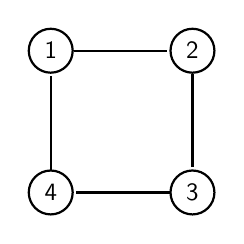
\begin{tikzpicture}[-,>=stealth,shorten >=1pt,auto,node distance=2cm,thick,main node/.style={scale=0.9,circle,draw,font=\sffamily\normalsize}]
                    \node[main node] (1){1};
                    \node[main node] (2)[right of = 1]{2};
                    \node[main node] (3)[below of = 2]{3};
                    \node[main node] (4)[left of = 3]{4};

                    \path[every node/.style={font=\sffamily\small}]
                        (1) edge (2)
                        (2) edge (3)
                        (3) edge (4)
                        (4) edge (1)
                        ;
                \end{tikzpicture}
            \end{tabular}
            &\qquad&
            \begin{tabular}{c}
                \includegraphics[scale=0.65]{images/emb_1.png}
            \end{tabular}
        \end{tabular}
        
        \caption{The graph $C_4$ and its embedding into $\R^2$.}
    \end{figure}

    It's easy to see that this embedding is isometrical from $d_{C_4}$ to $\ell_1$ since all distances are preserved. For the $\ell_2$ metric, instead, we notice that the diagonals aren't isometric:
    \[d_{C_4}(1,3) = 2 \quad\quad \ell_2(f(v_1), f(v_3)) = \ell_2 \rbk{\rbk{-\frac{1}{2}, \frac{1}{2}}, \rbk{\frac{1}{2}, -\frac{1}{2}}} = \sqrt{2}\]

    In particular, this embedding induces a distortion factor of at most $\sqrt{2}$. Indeed, it can be proven through the \textbf{Shortest Diagonal Lemma} that this distortion factor is the best we can achieve. To prove the lemma, we use a technique called \textit{sum of squares proof}: the idea is to show that one equation made of sums of squares is equivalent to the square of another equation, implying that the first equation must be always non-negative. Sum of squares proof are very easy to check once the second equation has been found. However, finding such equation is hard: common tools involve approximations based on \textit{Gröbner basis algorithms} constructed through SDPs.

    \begin{framedlem}{Shortest Diagonal Lemma}
        Given any four points $y_1, y_2, y_3, y_4 \in \R^d$, it holds that:
        \[\ell_2^2(y_1, y_3) + \ell_2^2(y_2, y_4) \leq \ell_2^2(y_1, y_2) + \ell_2^2(y_2, y_3) + \ell_2^2(y_3, y_4) + \ell_2^2(y_4, y_1)\]
    \end{framedlem}

    \begin{proof}
        We prove the lemma coordinate-by-coordinate. Fix $t \in [d]$. For each $i \in [4]$, let $z_i = y_{t,i}$ be the $t$-th coordinate of $y_{i}$.
        
        \textbf{Claim}: For all $t \in [d]$ it holds that:
        \[(z_1-z_4)^2 + (z_2-z_3)^2 + (z-3-z_4)^2 + (z_4-z_1)^2 - (z_1-z_3)^2 - (z_2-z_4)^2 = (z_1-z_2 + z_3 - z_4)^2\]

        \begin{proof}[Proof of the claim.]
            Proved by simply expanding both terms of the claim.
        \end{proof}
        
        Through the claim, we conclude that for each $t \in [d]$ it holds that:
        \[(z_1-z_4)^2 + (z_2-z_3)^2 + (z-3-z_4)^2 + (z_4-z_1)^2 - (z_1-z_3)^2 - (z_2-z_4)^2 = (z_1-z_2 + z_3 - z_4)^2 \geq 0\]

        Recalling that $\ell_2^2(y_i, y_j) = \sum_{t \in [d]} (y_{t,i} - y_{y,j})^2$, we conclude that:
        \[\ell_2^2(y_1, y_2) + \ell_2^2(y_2, y_3) + \ell_2^2(y_3, y_4) + \ell_2^2(y_4, y_1) - \ell_2^2(y_1, y_3) - \ell_2^2(y_2, y_4) \geq 0\]
    \end{proof}

    \begin{framedprop}{}
        Any embedding of the shortest path metric $d_{C_4}$ into $\ell_2$ over $\R^d$, for any $d \in \N$, has a distortion factor of at least $\sqrt{2}$.
    \end{framedprop}

    \begin{proof}
        Fix $d \in \N$. Suppose that $f : V(C_4) \to \R^d$ is an embedding of $d_{C_4}$ into $\ell_2$. Without loss of generality, assume that $f(i) = x_i$ for each $i \in [4]$. Let $M$ be the maximum $\ell_2$ edge length over all the points embedded into $\R^d$:
        \[M = \max(\ell_2(x_1, x_2), \ell_2(x_2, x_3), \ell_2(x_3, x_4), \ell_2(x_4, x_1))\]

        and let $m$ be the minimum $\ell_2$ diagonal length over all the points embedded into $\R^d$:
        \[m = \min(\ell_2(x_1, x_3), \ell_2(x_2,x_4))\]

        Through the Shortest Diagonal Lemma we have that:
        \[\begin{split}
            2m^2 &\leq \ell_2^2(y_1, y_3) + \ell_2^2(y_2, y_4) \\
            &\leq \ell_2^2(y_1, y_2) + \ell_2^2(y_2, y_3) + \ell_2^2(y_3, y_4) + \ell_2^2(y_4, y_1)\\
            & \leq 4M^2
        \end{split}\]

        concluding that $m \leq \sqrt{2}M$. Thus, since in $d_{C_4}$ the maximal edge length is 1 and the minimal diagonal length is 2, we conclude that the embedding $f$ must have applied a distortion factor of at least $\sqrt{2}$.
    \end{proof}

    \chapter{Submodular optimization}

    \section{Submodular functions}

    We consider a basic maximization problem, i.e. the \textbf{Max Cover problem}, where the goal is to cover as many elements as possible in a set-system. This problem clearly models many real-life situations, such as maximizing the number of satisfied users over a set of possible features to be added in an application.
    
    The Max Cover problem is formalizes similarly to the Minimum Set Cover problem. Given a number $n \in N$, let $\mathcal{U} = [n]$ be the universe set and let $\mathcal{C} = \{S_1, \ldots, S_m\}$ be a collection of subsets $S_i \subseteq \mathcal{U}$. Given a value $k \in \N$, the Max Cover problems asks us to find a sub-collection $\mathcal{S} \subseteq \mathcal{C}$ of $k$ sets that maximizes the number of covered elements in $\mathcal{U}$.
    \[\mathcal{S} = \{S_{i_1}^*, \ldots, S_{i_k}^*\} \in \argmax_{S_{i_1}, \ldots, S_{i_k} \in \mathcal{C}} \abs{\bigcup_{j \in [k]} S_{i_j}}\]

    This problem is one of the many problems that fall into the category of \textbf{submodular optimization}. We'll use this problem to build an intuition behind submodularity to then generalize the learned concepts. The approximation of the Max Cover problem is \textit{solved}, meaning that the best known approximation ratio of $1-\frac{1}{e} \approx 0.63\ldots$ has been proven to be tight under $\mathsf{NP}$-hardness. Surprisingly, a trivial greedy algorithm suffices to reach such approximation.

    \begin{algorithm}[H]
        \caption{$\rbk{1-\frac{1}{e}}$-approximation for Max Cover}
        \textbf{Input:} an universe set $\mathcal{U}$ and a collection $\mathcal{C}$

        \textbf{Output:} a sub-collection $\mathcal{S}$ of $\mathcal{C}$
        \begin{algorithmic}[1]
            \Function{$\rbk{1-\frac{1}{e}}$-approx-max-cover}{$\mathcal{U}, \mathcal{C}$}
                \State $S \gets \varnothing$
                \State $T_0 \gets \varnothing$
                \For{$i \in [k]$}
                    \For{$S \in \mathcal{C}-\mathcal{S}$}
                        \State $\mathrm{sc}_{T_{i-1}}(S) = \abs{S-T_{i-1}}$
                        \Comment $\mathrm{sc}$ acts as a score function
                    \EndFor

                    \State $S_i \in \argmax\limits_{S \in \mathcal{C}-\mathcal{S}} \mathrm{sc}_{T_{i-1}}(S)$
                    \State $\mathcal{S} \gets \mathcal{S} \cup \{S_i\}$
                    \State $T_i \gets T_{i-1} \cup S_i$
                \EndFor
                \State Return $\mathcal{S}$
            \EndFunction
        \end{algorithmic}
    \end{algorithm}

    \begin{framedthm}{}
        Given an input $(\mathcal{U}, \mathcal{C})$ of the Max Cover problem, let $\mathcal{S}^*$ be an optimal solution to Max-Cover$(\mathcal{U}, \mathcal{C})$. Given the output $\mathcal{S}$ of $\rbk{1-\frac{1}{e}}$\textsc{-approx-max-cover}, it holds that 
        \[\abs{\bigcup_{S \in \mathcal{S}} S} \geq \rbk{1-\frac{1}{e}}  \abs{\bigcup_{S \in \mathcal{S}^*} S}\]
    \end{framedthm}

    \begin{proof}
        First, we introduce some notation. Let $S_1, \ldots, S_k$ be the sets selected by the algorithm and let $T_1, \ldots, T_k$ be the sets of covered elements on each iteration, i.e. $T_{i} \cup \cup_{j \in [i]} S_j$. Let $X^* = \bigcup_{S \in \mathcal{S}^*} S$ be the set of elements covered by the optimal solution. For each $i \in [k]$, let $\mu_i = \abs{X^*} - \abs{T_i}$ be the advantage of the optimal solution over the $i$-th iteration. 

        \textbf{Claim 1}: for all $i \in [k]$ it holds that $\abs{S_i-T_i} \geq \frac{\mu_{i-1}}{k}$

        \begin{proof}[Proof of Claim 1.]
            Fix $i \in [k]$. Since $\abs{\mathcal{S^*}} = k$, there must exist a set $S_j^* \in \mathcal{S^*}$ such that:
            \[\abs{S_j^*-T_{i-1}} \geq \frac{\abs{X^*}-\abs{T_{i-1}}}{k} = \frac{\mu_{i-1}}{k}\]
            since otherwise it would be impossible for $\mathcal{S^*}$ to cover all of $\mathcal{X^*}-T_{i-1}$.

            Hence, the set $S_i$ selected at the $i$-th iteration is at least as large as $S_j^*$, since it is the one maximizing the score over $T_{i-1}$:
            \[\mathrm{sc}_{T_{i-1}}(S_i) \geq \mathcal{sc}_{T_{i-1}}(S_j^*) \geq \frac{\mu_{i-1}}{k}\]

        \end{proof}

        \textbf{Claim 2}: for all $i \in [k]$ it holds that $\mu_i \geq \rbk{1-\frac{1}{k}}^i \abs{X^*}$

        \begin{proof}[Proof of Claim 2.]
            We proceed by induction on $i$. When $i = 0$, we trivially have that:
            \[\rbk{1-\frac{1}{k}}^0 \abs{X^*} = \abs{X^*} = \abs{X^*} - \abs{T_0} = \mu_0\]

            Assume that the claim is true for any $m \leq i$. Through some algebraic manipulation we get that:
            \[\begin{split}
                \mu_{i+1} &= \abs{X^*} - \abs{T_{i+1}} \\
                & = \abs{X^*} - \abs{\bigcup_{j \in [i+1]} S_i} \\
                & = \abs{X^*} - \rbk{\abs{\bigcup_{j \in [i]} S_i} + \abs{S_{i+1} - \bigcup_{j \in [i]} S_i}} \\
                & = \abs{X^*} - \rbk{\abs{T_i} + \abs{S_{i+1} - T_i}} \\
                & = \mu_i - \abs{S_{i+1} - T_i} \\
            \end{split}\]

            Through Claim 1 we get that:
            \[\mu_{i+1} = \mu_i - \abs{S_{i+1} - T_i} \leq \mu_i - \frac{\mu_i}{k} = \rbk{1-\frac{1}{k}} \mu_i\]

            Finally, through inductive hypothesis we conclude that:
            \[\mu_{i+1} \leq \rbk{1-\frac{1}{k}} \mu_i \leq \rbk{1-\frac{1}{k}}^{i+1} \abs{X^*}\]
        \end{proof}

        Recalling that $\rbk{1-\frac{1}{x}} \leq e^{-1}$ for all $x \in \R^+$, through Claim 2 we conclude that:
        \[\abs{X^*} - \abs{T_k} = \mu_k \leq \rbk{1-\frac{1}{k}}^{k} \abs{X^*} \leq e^{-1}\abs{X^*}\]
        which implies that:
        \[\abs{T_k} \geq \rbk{1-\frac{1}{e}} \abs{X^*}\]

        Since $T_k$ contains all the elements covered by $\mathcal{S}$, this concludes the proof.
    \end{proof}

    The max cover problem is the typical example of a \textbf{submodular function},  a set function that, informally, describes the relationship between a set of inputs and an output, where adding more of one input has a decreasing additional benefit. As we'll discuss in this section, submodular functions are of fundamental interest in mathematics, economics and computer science: most optimization problems actually deal with submodular functions.

    \begin{frameddefn}{Modular functions}
        Given $n \in \N$, let $f : \mathcal{P}([n]) \to \R$ be a set function. We say that $f$ is:
        \begin{itemize}
            \item a \textbf{submodular function} when $\forall S,T \subseteq [n] \;\; f(S) + f(T) \geq f(S \cup T) + f(S \cap T)$
            \item a \textbf{modular function} when $\forall S,T \subseteq [n] \;\; f(S) + f(T) = f(S \cup T) + f(S \cap T)$
            \item a \textbf{supermodular function} when $\forall S,T \subseteq [n] \;\; f(S) + f(T) \leq f(S \cup T) + f(S \cap T)$
        \end{itemize}
    \end{frameddefn}

    We observe that the main property of submodular, modular and supermodular functions is the property to know the full description of the function through at most $n+1$ values. For instance, if $f$ is modular then the value of $f(\{1,2, 3\})$ can be computed through $f(\varnothing), f(\{1\}), f(\{2\})$ and $f(\{3\})$:
    \[f(\{1,2,3\}) = f(\{1,2\}) + f(\{3\}) - f(\varnothing) = f(\{1\}) + f(\{2\}) - f(\varnothing) + f(\{3\}) - f(\varnothing)\]

    \begin{framedprop}{}
        Given $n  \in \N$, the function $f : \mathcal{P}([n]) \to \R$ is submodular if and only if $\exists z, w_1, \ldots, w_n$ such that $\forall S \subseteq [n]$ it holds that $f(S) = z + \sum_{i \in S} w_i$.
    \end{framedprop}

    \begin{proof}
        Suppose that $f$ is modular and fix a set $S \subseteq [n]$. Assume that $S = \{1, \ldots, k\}$. By modularity we have that:
        \[\begin{split}
            f(S) &= f(\{1, \ldots k\}) \\
            &= f(\{2, \ldots, k\}) + f(\{1\}) - f(\varnothing) \\
            &= f(\{3, \ldots, k\}) + f(\{1\}) - f(\varnothing) + f(\{2\}) - f(\varnothing) \\
            &= f(\varnothing) + \sum_{i \in S} (f(\{i\}) - f(\varnothing))\\
            &= z + \sum_{i \in S} w_i
        \end{split}\]

        where $z = f(\varnothing)$ and $w_i = f(\{i\}) - f(\varnothing)$. Vice versa, suppose that $\exists z', w_1', \ldots, w_n'$ such that $\forall S \subseteq [n]$ it holds that $f(S) = z' + \sum_{i \in S} w_i'$. Fix two sets $S,T \subseteq [n]$. Then we have that:
        \[\begin{split}
            f(S) + f(T) &= z' + \sum_{i \in S} w_i' + z + \sum_{i \in T} w_i' \\
            &= z' + \sum_{i \in S \cap T} w_i' + \sum_{i \in S-T} w_i' + z + \sum_{i \in S \cap T} w_i' + \sum_{i \in T-S} w_i' \\
            &= \rbk{z' + \sum_{i \in S \cap T} w_i'} + \rbk{z + \sum_{i \in S-T} w_i' + \sum_{i \in S \cap T} w_i' + \sum_{i \in T-S} w_i'} \\
            &= f(S \cap T) + f(S \cup T)
        \end{split}\]
        hence $f$ is submodular.
    \end{proof}

    When a property holds for submodular functions, it's often the case that the respective property also holds supermodular ones (e.g. the property is the same but the inequality is inverted). The reason behind submodularity's importance in optimization problems derives from it's natural diminishing return property. In economics, \textbf{diminishing returns} referres to the decrease in incremental output of a production process as the amount of a single factor of production is incrementally increased, holding all other factors of production equal. In other words, the lesser the amount of elements, the better the return.
    
    \begin{frameddefn}{Diminishing return}
        Given $n  \in \N$, let $f : \mathcal{P}([n]) \to \R$. Given $S \subseteq [n]$ and $x \in [n]-S$, we define the \textbf{return} of $x$ on $S$ for $f$ as:
        \[\Delta_f(x \mid S) = f(S \cup \{x\}) - f(S)\]

        We say that $f$ has \textbf{diminishing return} when $\forall A \subseteq B \subseteq [n]$ and $\forall x \in [n] - B$ it holds that:
        \[\Delta_f(x \mid A) \geq \Delta_f(x \mid B)\]
    \end{frameddefn}

    \begin{framedthm}[label={sub_dim_ret}]{}
        Given $n  \in \N$, let $f : \mathcal{P}([n]) \to \R$. Then, $f$ is submodular if and only if it has diminishing return.
    \end{framedthm}

    \begin{proof}
        Suppose that $f$ is submodular. Fix any $A \subseteq B \subseteq [n]$ and any $x \in [n] - B$. By submodularity, we have that:
        \[f(A \cup \{x\}) + f(B) \geq f(A \cup B \cup \{x\}) + f((A \cup \{x\}) \cap B)\]

        Since $A \subseteq B$ and $x \notin B$, we get that:
        \[f(A \cup \{x\}) + f(B) \geq f(B \cup \{x\}) + f(A)\]

        Through some algebraic manipulation, we get that:
        \[\Delta_f(x \mid A) = f(A \cup \{x\}) - f(A) \geq f(B \cup \{x\}) - f(B) = \Delta_f(x \mid B)\]

        The other implication is left as an exercise (see \Cref{solved_submod}).
    \end{proof}
    
    In the previous section, we briefly mentioned that the Max-Cover problem is a submodular optimization problem, which means that the problem can be described in terms of a submodular function. Given a number $t \in N$, let $\mathcal{U} = [t]$ be the universe set and let $\mathcal{C} = \{A_1, \ldots, A_n\}$ be a collection of subsets $A_i \subseteq \mathcal{U}$. We define the \textbf{covering function} $f : \mathcal{P}([n]) \to \R$ as:
    \[f(S) = \abs{\bigcup_{i \in S} A_j}\]

    \begin{framedprop}{}
        The covering function is non-negative, monotone increasing and submodular.
    \end{framedprop}

    \begin{proof}
        Given any set $X \subseteq [n]$, we observe that:
        \[f(X) = \sum_{i \in [t]} \1[\exists j \in X \; i \in A_j] = \sum_{i \in [t]} f_i(X)\]

        where for each $i \in [t]$ the subfunction $f_i : \mathcal{P}([n]) \to \R$ is defined as:
        \[f_i(X) = \soe{ll}{
            1 & \exists j \in X \; i \in A_j \\
            0 & \text{otherwise}
        }\]

        \textbf{Claim:} for all $i \in [t]$ the subfunction $f_i$ is non-negative, monotone increasing and submodular.

        \begin{proof}
            Fix $S,T \subseteq [n]$. By definition, we trivially have that $f_i$ is non-negative, which implies that $f_i(S) + f_i(T) \leq 0$. Moreover, by definition $f_i$ is also monotone increasing, meaning that if $S \subseteq T$ then $f_i(S) \leq f_i(T)$. Hence, since $S \cap T \subseteq S \cup T$ and $f_i$ is non-negative, we have only two cases:
            \begin{enumerate}
                \item $f_i(S \cup T) = f_i(S \cap T) = 1$. Then, there is a $j \in S \cap T$ such that $i \in A_j$, which implies that $f_i(S) = f_i(T) = 1$. Hence, we have that:
                \[f_i(S) + f_i(T) = 1+1 = f_i(S \cup T) + f_i(S \cap T)\]

                \item $f_i(S \cup T) =1$ but $f_i(S \cap T) = 0$. Then, there is a $j \in S \cup T$ such that $i \in A_j$, which implies that $f_i(S) + f_i(T) \geq 1$. Hence, we have that:
                \[f_i(S) + f_i(T) \geq 1 = f_i(S \cup T) + f_i(S \cap T)\]
            \end{enumerate}
        \end{proof}

        Fix $S,T \subseteq [n]$. Through the claim, $f$ is trivially non-negative and monotone increasing. Moreover, we have that:
        \[\begin{split}
            f(S) + f(T) &= \sum_{i \in [t]} f_i(S) + f_i(T) \\
            &\geq \sum_{i \in [t]} f_i(S \cup T) + f_i(S \cap T) \\
            &= \sum_{i \in [t]} f_i(S \cup T) + \sum_{i \in [t]} f_i(S \cap T) \\
            &= f(S \cup T) + f(S \cap T)
        \end{split}\]

        thus $f$ is also submodular.
    \end{proof}

    Since the Max-Cover problem is $\mathsf{NP}$-hard, through the previous proposition we get that the general problem of maximizing a non-negative, monotone increasing, submodular function over $k$ elements is $\mathsf{NP}$-hard. In fact, the $\rbk{1-\frac{1}{e}}$-approximation for the Max-Cover problem that we discussed in the previous section is a specific instance of the more general $\rbk{1-\frac{1}{e}}$-approximation algorithm, developed by \textcite{nemhauser}, for the general probem that aims to maximize a NN-MI (non-negative, monotone increasing) submodular function.

    \begin{algorithm}[H]
        \caption{NWF $\rbk{1-\frac{1}{e}}$-approximation}
        \textbf{Input:} a NN-MI submodular function $f : \mathcal{P}(X) \to \R$  and a value $k \in \N$

        \textbf{Output:} a subset $S \subseteq X$
        \begin{algorithmic}[1]
            \Function{NWF-$\rbk{1-\frac{1}{e}}$-approx}{$f,$}
                \State $S_0 \gets \varnothing$
                \For{$i \in [k]$}
                    \State $x_{i+1} \in \argmax\limits_{X-S_i} f(S_i \cup \{x\})$
                    \Comment Or, equivalently, maximize $\Delta_f(x_{i+1} \mid S_i)$
                    \State $S_{i+1} \gets s_{i} \cup \{x_{i+1}\}$
                \EndFor
                \State Return $\mathcal{S_k}$
            \EndFunction
        \end{algorithmic}
    \end{algorithm}

    \begin{framedthm}{}
        Consider a non-negative, monotone increasing, submodular function $f : \mathcal{P}(X) \to \R$ and a value $k$. Given the output $S$ of \textsc{NWF-}$\rbk{1-\frac{1}{e}}$\textsc{-approx}, it holds that:
        \[f(S) \geq \rbk{1-\frac{1}{e}} \max\limits_{S \in \binom{X}{k}} f(S)\]
    \end{framedthm}

    \begin{proof}
        The proof is a generalization of the one of Max-Cover's approximation. Let $S^* = \{x_1^*, \ldots, x_k^*\}$ be an optimal solution, i.e. $S^* \in \argmax\limits_{S \in \binom{X}{k}} f(S)$

        \textbf{Claim 1}: for any $i \in [k-1]$ it holds that $f(S^*) \leq f(S_i) + k(f(S_{i+1}) - f(S_i))$

        \begin{proof}[Proof of Claim 1.]
            Since $f$ is monotone increasing, we observe that $f(S^*) \leq f(S_i \cup S^*)$. Through some algebraic manipulation, we're able to explicit a sum of return values by adding and subtracting values:
            \[\begin{split}
                f(S^*) &\leq f(S_i \cup S^*) \\
                &= f\rbk{S_i \cup \bigcup_{i = 0}^{k} \{x_i^*\}} \\
                &= f\rbk{S_i \cup \bigcup_{i = 0}^{k} \{x_i^*\}} + \sum_{j = 0}^{k-1} \rbk{-f\rbk{S_i \cup \bigcup_{i = 0}^{j} \{x_i^*\}} + f\rbk{S_i \cup \bigcup_{i = 0}^{j} \{x_i^*\}}} \\
                &= \sum_{j = 0}^k \rbk{f\rbk{S_i \cup \bigcup_{i = 0}^{j} \{x_i^*\}} - f\rbk{S_i \cup \bigcup_{i = 0}^{j-1} \{x_i^*\}}} + f\rbk{S_i}\\
                &= \sum_{j = 0}^k \Delta_f\rbk{x_j^* \mid S_i \cup \bigcup_{i = 0}^{j} \{x_i^*\}} + f\rbk{S_i}\\
            \end{split}\]

            By \Cref{sub_dim_ret}, we know that $f$ is submodular if and only if it has diminishing return, hence:
            \[\begin{split}
                f(S^*) &\leq \rbk{S_i} + \sum_{j = 0}^k \Delta_f\rbk{x_j^* \mid S_i \cup \bigcup_{i = 0}^{j} \{x_i^*\}} \\
                &\leq \rbk{S_i} + \sum_{j = 0}^k \Delta_f\rbk{x_j^* \mid S_i} \\
            \end{split}\]

            By the greedy choice of the algorithm, we conclude that:
            \[\begin{split}
                f(S^*) &\leq \rbk{S_i} + \sum_{j = 0}^k \Delta_f\rbk{x_j^* \mid S_i}  \\
                &\leq \rbk{S_i} + \sum_{j = 0}^k \Delta_f\rbk{x_{i+1} \mid S_i} \\
                &= f(S_i) + k(f(S_i \cup \{x_{i+1}\}) - f(S_i)) \\
                &= f(S_i) + k(f(S_{i+1}) - f(S_i)) \\
            \end{split}\]
        \end{proof}

        The second part of the proof is identical to the one of Max-Cover. For each $i \in [k]$, let $\delta_i = f(S^*) - f(S_i)$.

        \textbf{Claim 2}: for all $i \in [k]$ it holds that $\delta_i \geq \rbk{1-\frac{1}{k}}^i f(S^*)$

        \begin{proof}[Proof of Claim 2.]
            We proceed by induction on $i$. When $i = 0$, we trivially have that:
            \[\rbk{1-\frac{1}{k}}^0 f(S^*) = f(S^*) = f(S^*) - f(S_0) = \delta_0\]

            Assume that the claim is true for any $m \leq i$. Through Claim 1, we have that:
            \[\begin{split}
                \delta_{i+1} &= f(S^*) - f(S_{i+1}) \\
                & \leq k(f(S_{i+1}) - f(S_i)) \\
                & = k(f(S_{i+1}) - f(S^*) + f(S^*) - f(S_i)) \\
                & = k(-\delta_{i+1} + \delta_i)
            \end{split}\]

            which implies that $\delta_{i+1} \leq \rbk{1-\frac{1}{k}} \delta_i$. Finally, through inductive hypothesis we conclude that:
            \[\delta_{i+1} \leq \rbk{1-\frac{1}{k}} \delta_i \leq \rbk{1-\frac{1}{k}}^{i+1} f(S^*)\]
        \end{proof}

        Recalling that $\rbk{1-\frac{1}{x}} \leq e^{-1}$ for all $x \in \R^+$, through Claim 2 we conclude that:
        \[f(S^*) - f(S_k) = \delta_k \leq \rbk{1-\frac{1}{k}}^{k} f(S^*) \leq e^{-1} f(S^*)\]
        which implies that:
        \[f(S_k) \geq \rbk{1-\frac{1}{e}} f(S^*)\]
    \end{proof}

    \section{Property variations}

    After discussing how any general non-negative, monotone increasing submodular function can be approximated with a $1 - \frac{1}{e}$ ratio, it's natural to ask if the approximation ratio changes when some of these properties are dropped. For example, we consider once again the Max-Cut problem. Given a graph $G$, we consider the \textbf{cut function}  $c : \mathcal{P}([n]) \to \R$ defined as $c(S) = \abs{\mathrm{cut}(S, \overline{S})}$, assuming that $V(G) = [n]$. 

    This function is also non-negative and submodular. However, it isn't monotone increasing: given two nodes $x,y \in V(K_3)$, we have that $\{x\} \subseteq \{x,y\}$ but $c(\{x\}) \geq c(\{x,y\})$. Nonetheless, this function has an additional property that makes it interesting, that being symmetry.

    \begin{framedprop}{}
        The cut function is non-negative, symmetric and submodular.
    \end{framedprop}

    \begin{proof}
        The non-negativy and symmetry of the function follow from its very definition. 

        Hence, we can focus on proving that it is submodular. Fix two sets $S,T \subseteq [n]$. We define the sets $A_{S}, A_{T}, A_{S,T}, A$ as follows:
        \[A_S = S-T \quad A_T = T-S \quad A_{S,T} = S \cap T \quad A = [n]-(S \cup T)\]

        The cut-set from $S$ to $\overline{S}$ can be partitioned into four disjoint cut-sets:
        \[\mathrm{cut}(S, \overline{S}) = \mathrm{cut}(A_S, A_T) \cup \mathrm{cut}(A_S, A) \cup \mathrm{cut}(A_{S,T}, A_T) \cup \mathrm{cut}(A_{S,T}, A)\]

        Hence, we get that:
        \[c(S) = \abs{\mathrm{cut}(A_S, A_T)} + \abs{\mathrm{cut}(A_{S}, A)} + \abs{\mathrm{cut}(A_{S,T}, A_T)} + \abs{\mathrm{cut}(A_{S,T}, A)}\]

        Similarly, we get that:
        \[\begin{split}
            c(T) &= \abs{\mathrm{cut}(A_T, A_S)} + \abs{\mathrm{cut}(A_{T}, A)} + \abs{\mathrm{cut}(A_{S,T}, A_S)} + \abs{\mathrm{cut}(A_{S,T}, A)} \\
            c(S \cup T) &= \abs{\mathrm{cut}(A_{S}, A)} + \abs{\mathrm{cut}(A_{T}, A)} + \abs{\mathrm{cut}(A_{S,T}, A)} \\
            c(S \cap T) &= \abs{\mathrm{cut}(A_{S,T}, A_S)} + \abs{\mathrm{cut}(A_{S,T}, A_T)} + \abs{\mathrm{cut}(A_{S,T}, A)}
        \end{split}\]

        concluding that:
        \[c(S) + c(T) = c(S \cup T) + c(S \cap T) + 2\abs{\mathrm{cut}(A_S, A_T)} \geq c(S \cup T) + c(S \cap T)\]
        implying that $c$ is submodular.
    \end{proof}

    \textcite{feige} proved that the trivial $\frac{1}{2}$-approximation that we discussed for Max-Cut can be generalized to any function satisfying the same properties of the cut function. Even thought Max-Cut has a better approximation ratio given by the GW algorithm, for generic functions this bound is actually thight.

    \begin{framedlem}{}
        Let $f$ be a submodular function. Then, for any pair $S_1, S_2 \subseteq [n]$ it holds that:
        \[\avg_{T_1 \subseteq S_1} \avg_{T_2 \subseteq S_2} f(T_1 \cup T_2) \geq \frac{f(\varnothing) + f(S_1) + f(S_2) + f(S_1 \cup S_2)}{4}\]
    \end{framedlem}

    \begin{proof}
        We start by claiming a restricted version of the lemma, which will be used to prove the lemma itself. In particular, it's easy to see that this claim is a special case of the whole lemma, where  $S_1 = S$ and $S_2 = \varnothing$.

        \textbf{Claim 1}: If $g$ is a submodular function then for any $S \subseteq [n]$ it holds that:
        \[\avg_{T \subseteq S} g(T_1 \cup T_2) \geq \frac{g(\varnothing) + g(S)}{2}\]

        \begin{proof}[Proof of Claim 1.]
            We proceed by induction on $\abs{S}$. For $\abs{S} = 0$ we have that $S = \varnothing$, thus the claim holds on equality. Consider the case where $\abs{S} = i+1$. Given an element $x \in S$, let $S' = S - \{x\}$. Through some algebraic manipulation we get that:
            \[\begin{split}
                \sum_{T \subseteq S}{g(T)} &= \sum_{T' \subseteq S'}{g(T')} + \sum_{T' \subseteq S'}{g(T' \cup \{x\})} \\
                &= \sum_{T' \subseteq S'}{g(T')} + \sum_{T' \subseteq S'}{g(T' \cup \{x\})} + \sum_{T' \subseteq S'}{g(T')} - \sum_{T' \subseteq S'}{g(T')} \\
                &= 2\sum_{T' \subseteq S'}{g(T')} + \sum_{T' \subseteq S'}{(g(T' \cup \{x\}) - g(T'))} \\
                &= 2\sum_{T' \subseteq S'}{g(T')} + \sum_{\substack{T \subseteq S : \\ x \in T}}{(g(T) - g(T \cap S'))} \\
            \end{split}\]
            
            By submodularity of $f$, we get that:
            \[\begin{split}
                \sum_{T \subseteq S}{g(T)} &= 2\sum_{T' \subseteq S'}{g(T')} + \sum_{\substack{T \subseteq S : \\ x \in T}}{(g(T) - g(T \cap S'))} \\
                &\ge 2\sum_{T' \subseteq S'}{g(T')} + \sum_{\substack{T \subseteq S : \\ x \in T}}{(g(T \cup S') - g(S'))} \\
                &= 2\sum_{T' \subseteq S'}{g(T')} + \sum_{\substack{T \subseteq S : \\ x \in T}}{(g(S) - g(S'))} \\
                &= 2\sum_{T' \subseteq S'}{g(T')} + 2^i(g(S) - g(S')) \\
            \end{split}\]

            By multiplying both sides of the inequality by $2^{- \abs S}$, we get that:
            \[\avg_{T \subseteq S}{g(T)} = 2^{- \abs S}\sum_{T \subseteq S}{g(T)} \ge 2 ^{1 - \abs S}\sum_{T' \subseteq S'}{g(T')} + 2^{i - \abs S}(g(S) - g(S'))\]
            
            Finally, through inductive hypothesis we conclude that:
            \[\begin{split}
                \avg_{T \subseteq S}{g(T)} &\ge 2^{- i}\sum_{T' \subseteq S'}{g(T')} + 2^{-1}(g(S) - g(S')) \\
                &= \avg_{T' \subseteq S'}{g(T')} + \dfrac{g(S) - g(S')}{2} \\
                &\ge \dfrac{g(\varnothing) + g(S')}{2} + \dfrac{g(S) - g(S')}{2} \\
                &= \dfrac{g(\varnothing) + g(S)}{2}
            \end{split}\]
        \end{proof}

        For any subset $X \subseteq [n]$, we define the function $h_X : \mathcal{P}([n]) \to \R : T \mapsto f(X \cup T)$.

        \textbf{Claim 2}: for any $X \subseteq [n]$, the function $h_X$ is submodular.

        \begin{proof}[Proof of Claim 2.]
            Given any pair $A, B \subseteq [n]$, we have that:
            \[\begin{split}
                h_X(A) + h_X(B) &= f(X \cup A) + f(X \cup B) \\
                &\ge f(X \cup A \cup B) + f((X \cup A) \cap (X \cup B)) \\
                &= f(X \cup A \cup B) + f(X \cup (A \cap B)) \\
                &= h_X(A \cup B) + h_X(A \cap B)
            \end{split}\]
        \end{proof}

        Since $h_X$ is submodular, by the previous lemma $\forall S \subseteq [n]$ it holds that:
        \[\avg_{T \subseteq S}{h_X(T)} \ge \dfrac{h_X(\varnothing) + h_X(S)}{2} = \dfrac{f(X) + f(X \cup S)}{2}\]
        
        Therefore, for any pair $S_1, S_2 \subseteq [n]$ we have that:
        \[\begin{split}
            \avg_{T_1 \subseteq S_1}{\avg_{T_2 \subseteq S_2}{f(T_1 \cup T_2)}} &= \avg_{T_1 \subseteq S_1}{\avg_{T_2 \subseteq S_2}{h_{T_1}(T_2)}} \\
            &\ge \avg_{T_1 \subseteq S_1}{\dfrac{f(T_1) + f(T_1 \cup S_2)}{2}}\\
            &= \dfrac{1}{2}\rbk{\avg_{T_1 \subseteq S_1}{f(T_1)} + \avg_{T_1 \subseteq S_1}{f(T_1 \cup S_2)}} \\
            &= \dfrac{1}{2} \rbk{\avg_{T_1 \subseteq S_1}{f(T_1)} + \avg_{T_1 \subseteq S_1}{h_{S_2}(T_1)}}
        \end{split}\]

        Through the two claims, we conclude that:
        \[\begin{split}
            \avg_{T_1 \subseteq S_1}{\avg_{T_2 \subseteq S_2}{f(T_1 \cup T_2)}} &= \dfrac{1}{2} \rbk{\avg_{T_1 \subseteq S_1}{f(T_1)} + \avg_{T_1 \subseteq S_1}{h_{S_2}(T_1)}} \\
            &\ge \dfrac{1}{2} \rbk{\dfrac{f(\varnothing) + f(S_1)}{2} + \dfrac{f(S_2) + f(S_2 \cup S_1)}{2}} \\
            &= \dfrac{f(\varnothing) + f(S_1) + f(S_2) + f(S_1 \cup S_2)}{4}
        \end{split}\]
    \end{proof}

    \begin{framedthm}{}
        Consider a non-negative, symmetric, submodular function $f : \mathcal{P}([n]) \to \R$ and a value $k$. Given a uniform at random subset $R \subseteq [n]$, it holds that:
        \[\Exp[f(R)] \geq \frac{1}{2} \max\limits_{S \in \binom{X}{k}} f(S)\]
    \end{framedthm}

    \begin{proof}
        Let $S^* = \{x_1^*, \ldots, x_k^*\}$ be an optimal solution, i.e. $S^* \in \argmax\limits_{S \in \binom{X}{k}} f(S)$. Through the previous lemma we know that:
        \[\begin{split}
            \dfrac{f(\varnothing) + f(S^*) + f([n]-S^*) + f([n])}{4} &\leq  \avg_{T_1 \subseteq S_1}{\avg_{T_2 \subseteq S_2}{f(T_1 \cup T_2)}} \\
            &= = 2^{- \abs{S^*}} \cdot 2^{- n + \abs{S^*}} \cdot \sum_{T_1 \subseteq S^*}{\sum_{T_2 \subseteq [n] - S^*}{f(T_1 \cup T_2)}} \\
            &= 2^{-n} \sum_{T_1 \subseteq S^*}{\sum_{T_2 \subseteq [n] - S^*}{f(T_1 \cup T_2)}} \\
            &= 2^ {-n} \sum_{T \subseteq S^* \cup ([n] - S^*)}{f(T)} \\
            &= 2^{-n} \sum_{T \subseteq [n]}{f(T)} \\
            &= \avg_{T \subseteq [n]}{f(T)} \\
            &= \Exp [f(R)]
        \end{split}\]

        Since $f$ is non-negative and symmetric, we conclude that:
        \[\begin{split}
            \Exp[f(R)] &\geq \dfrac{f(\varnothing) + f(S^*) + f([n]-S^*) + f([n])}{4} \\
            &\geq \dfrac{f(S^*) + f([n]-S^*)}{4} \\
            &= \dfrac{2f(S^*)}{4} \\
            &= \dfrac{1f(S^*)}{2} \\
        \end{split}\]
    \end{proof}

    We observe that the previous proof can also be adapted for functions that are non-negative, submodular but not symmetric by replacing the application of symmetry with another application of non-negativity, obtaining a $\frac{1}{4}$-approximation. 

    \begin{framedthm}{}
        Consider a non-negative, submodular function $f : \mathcal{P}([n]) \to \R$ and a value $k$. Given a uniform at random subset $R \subseteq [n]$, it holds that:
        \[\Exp[f(R)] \geq \frac{1}{4} \max\limits_{S \in \binom{X}{k}} f(S)\]
    \end{framedthm}

    \newpage
    
    To recap, we proved that:
    \begin{itemize}
        \item All NN-MI submodular functions have a $\rbk{1-\frac{1}{e}}$-approximation.
        \item All NN-SYM submodular functions have a $\frac{1}{2}$-approximation.
        \item All NN submodular functions have a $\frac{1}{4}$-approximation.
    \end{itemize}

    Other approximations results are known for other property variations (see \cite{feige} for a table of known approximation ratios). Submodularity gives us a standard approximation bound to many $\mathsf{NP}$-hard maximization problems. The same results can be obtained for through supermodularity for many  $\mathsf{NP}$-hard minimization problems. 

    \chapter{Online algorithms}

    \section{The Maximum Bipartite Matching problem}

    Up until now, we have discussed the Maximal Matching problem in terms of its relations with other problems. In this section, instead, we'll focus on matching on \textbf{bipartite graphs}. These types of matchings are of particular interest due to how they describe many real-life situations. For instance, the problem of finding the optimal assignment of tasks to a group of employees can be solved by finding a maximum matching: we split the graph in two partitions, one with all the tasks and one with all the employees, connecting each employee to the tasks that he's capable of completing.

    \begin{figure}[H]
        \centering
        \resizebox{0.16\textwidth}{!}{
            \begin{tikzpicture}[-,>=stealth,shorten >=1pt,auto,node distance=2cm,thick,main node/.style={scale=1,circle,draw,font=\sffamily\normalsize}, rotate=90,transform shape]
                \node[main node] (1) [fill = Carmine,]{};
                \node[main node] (2) [fill = Carmine,right of=1] {};
                \node[main node] (3) [fill = Carmine,right of=2] {};
                \node[main node] (4) [fill = Carmine,right of=3] {};
                \node (5) [below right of=1] {};
                \node[main node] (6) [fill = BlueLagoon,below left of=5] {};
                \node[main node] (7) [fill = BlueLagoon,right of=6] {};
                \node[main node] (8) [fill = BlueLagoon,right of=7] {};
                \node[main node] (9) [fill = BlueLagoon,right of=8] {};

                \path[every node/.style={font=\sffamily\small}]
                        (1) edge (6)
                        (1) edge[color = Green, line width = 2] (9)
                        (2) edge (8)
                        (3) edge[color = Green, line width = 2] (6)
                        (3) edge (7)
                        (4) edge (8)
                        (4) edge (9)
                    ;
            \end{tikzpicture}
        }

        \caption{A matching on a bipartite graph.}
    \end{figure}

    Consider the matching on the bipartite graph shown in the previous figure. We observe that this matching is neither maximal nor maximum. When the matching is not maximal, we can obtain a matching with greater cardinality simply by extending it.

    \begin{figure}[H]
        \centering
        \resizebox{0.16\textwidth}{!}{
                \begin{tikzpicture}[-,>=stealth,shorten >=1pt,auto,node distance=2cm,thick,main node/.style={scale=1,circle,draw,font=\sffamily\normalsize}, rotate=90,transform shape]
                \node[main node] (1) [fill = Carmine,]{};
                \node[main node] (2) [fill = Carmine,right of=1] {};
                \node[main node] (3) [fill = Carmine,right of=2] {};
                \node[main node] (4) [fill = Carmine,right of=3] {};
                \node (5) [below right of=1] {};
                \node[main node] (6) [fill = BlueLagoon,below left of=5] {};
                \node[main node] (7) [fill = BlueLagoon,right of=6] {};
                \node[main node] (8) [fill = BlueLagoon,right of=7] {};
                \node[main node] (9) [fill = BlueLagoon,right of=8] {};

                \path[every node/.style={font=\sffamily\small}]
                        (1) edge (6)
                        (1) edge[color = Green, line width = 2] (9)
                        (2) edge (8)
                        (3) edge[color = Green, line width = 2] (6)
                        (3) edge (7)
                        (4) edge[color = Green, line width = 2] (8)
                        (4) edge (9)
                    ;
            \end{tikzpicture}
        }

        \caption{A maximal matching on a bipartite graph.}
    \end{figure}

    We notice that the above matching is maximal, but not maximum. For instance, we observe that the number of edges outside of the matching that we selected form new matching with more edges than the one that we have considered. Hence, by \textit{swapping} all the edges, we get a matching with higher cardinality. Moreover, this new matching is clearly a maximum one since the number of nodes is equal to twice the number of selected edges.

    \begin{figure}[H]
        \centering
        \resizebox{0.16\textwidth}{!}{
            \begin{tikzpicture}[-,>=stealth,shorten >=1pt,auto,node distance=2cm,thick,main node/.style={scale=1,circle,draw,font=\sffamily\normalsize}, rotate=90,transform shape]
                \node[main node] (1) [fill = Carmine,]{};
                \node[main node] (2) [fill = Carmine,right of=1] {};
                \node[main node] (3) [fill = Carmine,right of=2] {};
                \node[main node] (4) [fill = Carmine,right of=3] {};
                \node (5) [below right of=1] {};
                \node[main node] (6) [fill = BlueLagoon,below left of=5] {};
                \node[main node] (7) [fill = BlueLagoon,right of=6] {};
                \node[main node] (8) [fill = BlueLagoon,right of=7] {};
                \node[main node] (9) [fill = BlueLagoon,right of=8] {};

                \path[every node/.style={font=\sffamily\small}]
                        (1) edge[color = Green, line width = 2] (6)
                        (1) edge (9)
                        (2) edge[color = Green, line width = 2] (8)
                        (3) edge (6)
                        (3) edge[color = Green, line width = 2] (7)
                        (4) edge (8)
                        (4) edge[color = Green, line width = 2] (9)
                    ;
            \end{tikzpicture}
        }

        \caption{The maximum matching obtained by swapping all the edges.}
    \end{figure}

    Let's take a closer look to what we just did. We notice that all the edges of the last non-maximum matching actually form a path whose edges alternate between being outside of the matching and inside of the matching. Moreover, both the first and last edge of such path are outside of the matching, hence the number of outside edges is one more than the number of inside edges. We generalize such paths through the concept of \textit{alternating path} and \textit{augmenting path}.
    
    \begin{frameddefn}{Alternating and augmenting path}
        Let $G$ be a bipartite graph and let $M \subseteq E(G)$ be a matching on $G$. An \textbf{$M$-alternating path} is a path starting from an unmatched node and whose edges alternate between $M$ and $E(G)-M$. If the path also ends at an unmatched node, the path is said to be \textbf{$M$-augmenting}.
    \end{frameddefn}

    To clarify this definition, let's make things more formal. A path $P = x_0 e_1 x_1 e_2 \ldots e_k x_k$ is $M$-alternating when $x_0$ is unmatched, meaning that there is no edge $e \in M$ in the matching such that $x_0 \in e$, and whose edges alternate between being outside of the matching and inside of the matching, meaning that $e_1 \notin M, e_2 \in M, e_3 \notin M$ and so on. When $x_k$ is also unmatched, the path is said to be $M$-augmenting. This name comes from the fact that, in order for $x_k$ to be unmatched, the last edge is not inside the matching, meaning that we have more edges outside of the matching then inside of it. Moreover, since $x_0$ and $x_k$ are unmatched, by swapping the edges inside of the matching with the edges outside of it we're guaranteed to get a matching (with more edges than the previous one).

    \begin{figure}[H]
        \centering
        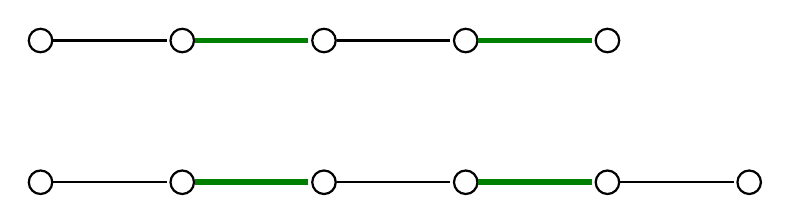
\begin{tikzpicture}[-,>=stealth,shorten >=1pt,auto,node distance=2cm,thick,main node/.style={scale=0.9,circle,draw,font=\sffamily\normalsize}]
            \node[main node] (1) []{};
            \node[main node] (2) [right of = 1]{};
            \node[main node] (3) [right of = 2]{};
            \node[main node] (4) [right of = 3]{};
            \node[main node] (5) [right of = 4]{};

            \node[main node] (6) [below of = 1]{};
            \node[main node] (7) [right of = 6]{};
            \node[main node] (8) [right of = 7]{};
            \node[main node] (9) [right of = 8]{};
            \node[main node] (10) [right of = 9]{};
            \node[main node] (11) [right of = 10]{};

            \path[every node/.style={font=\sffamily\small}]
                (1) edge (2)
                (2) edge[color = Green, line width = 2] (3)
                (3) edge (4)
                (4) edge[color = Green, line width = 2] (5)

                (6) edge (7)
                (7) edge[color = Green, line width = 2] (8)
                (8) edge (9)
                (9) edge[color = Green, line width = 2] (10)
                (10) edge (11)
            ;
        \end{tikzpicture}

        \caption{An $M$-alternating path (above) and an $M$-augmenting path (below).}
    \end{figure}

    \begin{framedlem}{}
        Let $G$ be a bipartite graph and let $M \subseteq E(G)$ be a matching on $G$. If $P$ is an $M$-augmenting path then $M \Delta E(P)$ is matching on $G$ with more edges than $M$
    \end{framedlem}

    \begin{proof}
        First, we recall that the \textit{symmetric difference} $M \Delta E(P)$ is defined as follows:
        \[M \Delta E(P) = (M \cup E(P)) - (M \cap E(P))\]

        Let $M' = M \Delta E(P)$. We observe that all the edges that aren't shared by $M$ and $P$ are also not in $M'$, hence we can ignore them. Let $P = x_0 e_1 x_1 e_2 \ldots e_k x_k$. Since $P$ is augmenting, the number of edges in $P$ that are also in $M$ is less than the number of edges that aren't in $M$. Hence, we get that $\abs{M'} > \abs{M}$.
    \end{proof}

    The above lemme gives us an easy way to increase the cardinality of our matching by finding augmenting paths and swapping edges. But how can we be sure that we have reached the maximum matching? \textcite{berge} proved that the above lemma can indeed be extended: if there are no augmenting paths then the matching is maximum.

    \begin{framedthm}[label={berge}]{Berge's theorem}
        Let $G$ be a bipartite graph and let $M \subseteq E(G)$ be a matching on $G$. Then, $M$ is a maximum matching on $G$ if and only if there are no $M$-augmenting paths.
    \end{framedthm}

    \begin{proof}
        One of the two implications directly follows from the previous lemma. For the other implication, we prove the contrapositive. Suppose that $M$ is a non-maximum matching on $G$. Then, there is at least one matching $M'$ on $G$ such that $\abs{M'} > \abs{M}$. Let $H \subseteq G$ be the graph such that $V(H) = V(G)$ and $E(H) = M \Delta M'$, where $\Delta$ denotes the \textit{symmetric difference}. We observe that every edge that is shared among $M$ and $M'$ gets deleted in $H$, hence we can ignore them.

        \textbf{Claim:} for every $x \in V(H)$ it holds that $\deg_H(x) \leq 2$.

        \begin{proof}[Proof of Claim 1.]
            Since $M$ and $M'$ are both matchings on $G$, each vertex can have at most one edge in $M$ and at most one edge in $M'$. If they share the same edge then $H$ won't contain such edge. If they don't, $x$ will have degree 2 in $H$.
        \end{proof}

        We observe that the above claim has many consequences. In particular, it implies that every component of $H$ must be either a cycle or a path (including trivial paths of one single vertex).
        
        \textbf{Claim 2}: every cycle component of $H$ has even length

        \begin{proof}[Proof of Claim 2.]
            By way of contradiction, suppose that there is a cycle $C$ of odd length. By construction, each component has to alternate between edges of $M$ and $M'$. Hence, at least one vertex of $C$ must have both edges lying either inside $M$ or $M'$, contradicting the fact that either $M$ or $M'$ is a matching. 
        \end{proof}

        Since $\abs{M'} > \abs{M}$, there must be a component with at least one (and at most one) edge in $M'$. Since the edges of each component alternate between $M$ and $M'$, by Claim 2 we know that such component cannot be a cycle. Hence, it must be a path component $P$. In order for $P$ to have more edges in $M'$ than edges in $M$, the first and last edge must be edges of $M'$, meaning that $P$ is an $M$-augmenting path. By contrapositive, if there is no $M$-augmenting path then $M$ is a maximum matching.
    \end{proof}

    This theorem has been used to construct many algorithms for finding a maximum matching on bipartite graphs, the easiest one being the following:

    \begin{algorithm}[H]
        \caption{Maximum Bipartite Matching}
        \textbf{Input:} a bipartite graph $G$ with partition $(V,W)$

        \textbf{Output:} a matching $M$ of $G$
        \begin{algorithmic}[1]
            \Function{max-bip-matching}{$G$}
                \State $M \gets \varnothing$
                \While{$\exists P \text{ $M$-augmenting path} $}
                    \State $M \gets M \Delta P$
                \EndWhile
                \State Return $M$
            \EndFunction
        \end{algorithmic}
    \end{algorithm}

    The augmenting path in this algorithm can be found through a DFS or BFS, making the runtime $O(mn)$. Some variants of this idea are able to reduce the runtime by efficiently computing augmenting paths, such as the \textbf{Hopcroft-Karp algorithm} \cite{hopcroft-karp}. Given a bipartite graph $G$ with bipartition $(A,B)$, the idea behind such algorithms is to run a simultaneous BFS starting from all the unmatched vertices of $A$, until at least
    one free node of $B$ is found. Then, we run a DFS over the forest produced by the BFS, starting from the unmatched nodes of $B$. Each path found through this procedure is an augmenting path, hence their edges can be swapped to increase the cardinality of the matching. The whole process is repeated until no augmenting path is found. This process guarantees a runtime of $O(m \sqrt{n})$. 
    
    \section{The Online approach}

    In computer science, an \textbf{online algorithm} is an algorithm whose input is fed piece-by-piece in a serial fashion, without having the entire input available from the start. In contrast, an \textbf{offline algorithm} -- the standard type of algorithm -- is given the whole input from the beginning and is required to output an answer which solves the problem at hand. Online algorithms allow the user to solve the problem \curlyquotes{as it comes}, making it unnecessary to know the whole input data. This type of algorithms became a fundamental topic of study as the Internet grew in usage, in particular with the advent of the \curlyquotes{big data} phenomena. These days, we require to solve problems that must work with huge amounts of data, making memory optimization an hard task even for high-end super-computers.
    
    For instance, the Maximum Bipartite Matching problem is a fundamental topic of study for \textit{advertisement services}. Suppose that an Internet ad services has to match each user to at most one advertisement per hour and each advertisement can be matched to at most one user per hour. Through analysis of their interests, the service constructs a list of potential ads to show to the user. To maximize the profits, the ad service wants to find the maximum matching between users and ads. It's easy to see that this is clearly equivalent to the Maximum Bipartite Matching problem, where users lie in one partition of the graph and ads lie on the other. However, there are two main problems:
    \begin{itemize}
        \item The amount of users and ads is too large, making storage a difficult task
        \item The set of users and ads changes over time, meaning that a previous match may not be optimal anymore
    \end{itemize}

    Online algorithms come at hand in both situations. However, since such algorithm doesn't know the whole input from the start, it is forced to make decisions that may later turn out not to be optimal. The study of online algorithms has focused on the \textbf{quality of decision-making} that is possible in this setting. For instance, suppose that our online algorithm currently knows the following graph, where the red nodes represent ads and the blue nodes represent users.

    \begin{figure}[H]
        \centering
        \resizebox{0.2\textwidth}{!}{
            \begin{tikzpicture}[-,>=stealth,shorten >=1pt,auto,node distance=2cm,thick,main node/.style={scale=1,circle,draw,font=\sffamily\normalsize}]
                \node[main node] (1) [fill = Carmine,text=white]{$A$};
                \node[main node] (2) [fill = Carmine, text=white, below of=1] {$B$};

                \node[main node] (3) [fill = BlueLagoon, text=white, right of=1, xshift=20] {$1$};

                \path[every node/.style={font=\sffamily\small}]
                        (1) edge (3)
                        (2) edge (3)
                    ;
            \end{tikzpicture}
        }

        \caption{A partial input known by an online bipartite matching algorithm.}
    \end{figure}

    Our algorithm has two possibilities: either match $1$ to $A$ or match it to $B$. Without loss of generality, assume that $1$ is matched to $A$. Suppose now that a new user $2$ joins the service. After analyzing their preferences, the system establishes that only the ad $A$ is compatible with user $2$, implying that the new user cannot be matched since $1$ is matched with $A$. However, if our algorithm had matched $1$ to $B$, we could've gotten a better matching.

    \begin{figure}[H]
        \centering
        \resizebox{0.2\textwidth}{!}{
            \begin{tikzpicture}[-,>=stealth,shorten >=1pt,auto,node distance=2cm,thick,main node/.style={scale=1,circle,draw,font=\sffamily\normalsize}]
                \node[main node] (1) [fill = Carmine, text=white]{$A$};
                \node[main node] (2) [fill = Carmine, text=white, below of=1] {$B$};

                \node[main node] (3) [fill = BlueLagoon, text=white, right of=1, xshift=20] {$1$};
                \node[main node] (4) [fill = BlueLagoon, text=white, below of=3] {$2$};

                \path[every node/.style={font=\sffamily\small}]
                        (1) edge[color = Green, line width = 2] (3)
                        (2) edge (3)
                        (1) edge (4)
                    ;
            \end{tikzpicture}
        }

        \caption{The new partial input when the second user joins.}
    \end{figure}

    This non-optimal-extension characteristic of algorithms is typical of online algorithms and it is often impossible to solve. For this reason, online algorithms are studied under the lens of \textbf{competitive analysis}, which compares the performance of an optimal offline algorithm (which can view the sequence of requests in advance) with respect to an online algorithm (which must satisfy an unpredictable sequence of requests, completing each request without being able to see the future). Unlike traditional worst-case analysis, where the performance of an algorithm is measured only for \curlyquotes{hard} inputs, competitive analysis requires that an algorithm perform well both on hard and easy inputs, where \curlyquotes{hard} and \curlyquotes{easy} are defined by the performance of the optimal offline algorithm. To measure the competitiveness of online algorithms, we use the \textbf{adversary model}, where an adversary feeds \curlyquotes{bad input} to the algorithm. For deterministic algorithms, the adversary is considered to be \textit{all-knowing}, meaning that they know how the online algorithm works. Since the latter cannot see into the future, an all-knowing adversary is able to fool the online algorithm.
    
    \begin{framedthm}{}
        There is no deterministic online algorithm for the Maximum Bipartite Matching problem that can match more than $\frac{1}{2}$ of the edges of an optimal solution.
    \end{framedthm}

    \begin{proof}
        We give an adversarial argument through an all-knowing adversary. The idea is to build a counterexample to any possible choice made by the online algorithm. On the first round, the adversary sends three vertices $a,b,x$ and two edges $\{a,x\}, \{b,x\}$. The online algorithm has three possible choices: leave $x$ unmatched, match it with $a$, or match it with $b$.
        
        If the algorithm matches $x$ with $a$, on the next round the adversary sends a new vertex $y$, an edge $\{a,y\}$ and then a message that signals that the input is terminated. Since $x$ is matched to $a$, the new vertex $y$ cannot be matched, meaning that the algorithm returns a solution with only one edge in the matching. However, an offline optimal solution would give a matching with two edges: $\{b,x\}$ and $\{a,y\}$, concluding that the the competitive ratio is $\frac{1}{2}$. If the algorithm matches $x$ with $b$, through a similar argument we can conclude that the the competitive ratio is $\frac{1}{2}$.

        Suppose now that the algorithm leaves $x$ unmatched. On the next round, the adversary sends a new vertex $y$, an edge $\{a,y\}$ (or an $\{b,y\}$) and then a message that signals that the input is terminated. If algorithm matches the vertex $y$ with $a$, the ratio is still $\frac{1}{2}$ since $x$ was left unmatched. If it leaves it unmatched, instead, the ratio is $0$. This concludes that the competitive ratio can be at most $\frac{1}{2}$.
    \end{proof}

    This results establishes an approximation ratio upper bound on every possible deterministic online algorithm, concluding that a perfect solutions is impossible for the Maximum (Bipartite) Matching problem. Knowing this, we shift our focus on finding a greedy solution that reaches such maximum approximation ratio. As in many cases, the best solution is the most obvious one: when a new user comes, we match if it's possible, otherwise we leave it unmatched and proceed with the next round. It's easy to see that such algorithm is actually solving the Maxim\underline{al} Bipartite Matching problem.

    \begin{algorithm}[H]
        \caption{The online maximal matching algorithm}
        \textbf{Input:} an undirected graph $G$ fed in an online way

        \textbf{Output:} a maximal matching $M$ of $G$

        \begin{algorithmic}[1]
            \Function{online-maximal-matching}{$G$}
                \State $M \gets \varnothing$
                \While{there is a new user $x$}
                    \State Read $N(x)$
                    \State $U(x) \gets \{v \in N(x) \mid \nexists e \in M \text{ s.t. } v \in e\}$
                    \If{$U(x) \neq \varnothing$}
                        \State Let $y$ be a random vertex in $U(x)$
                        \State{$M \gets M \cup \{x,y\}$}
                    \EndIf
                \EndWhile
                \State Return $M$
            \EndFunction
        \end{algorithmic}
    \end{algorithm}

    \begin{framedprop}{}
        Let $G$ be a graph. If $M^*$ is a maximum matching on $G$ and $M$ is a maximal matching on $G$ then $\abs{M} \geq \frac{1}{2} \abs{M^*}$.
    \end{framedprop}

    \begin{proof}
        Let $S = \{v \in V(G) \mid \exists e \in M \text{ s.t. } v \in e\}$. By construction, $\abs{S} = 2\abs{M}$. Each $e \in M^*$ is incident to at least one edge of $S$, since otherwise $M \cup \{e\}$ is a matching that extends $M$. Moreover, each node of $S$ is incident to at most one edge of $S$, otherwise $M^*$ is not a matching. Hence, there is a function $f : M^* \to S$ with $f(e) \in S \cap e$ that is also injective, concluding that $\abs{M^*} \leq \abs{S} = 2\abs{M}$.
    \end{proof}

    The above proposition and the previous theorem conclude that our online greedy algorithm is an optimal approximation for the Maximum Matching problem.
    
    To mitigate the limits of deterministic online algorithms, \textit{randomness} can often come at hand. In the case of randomized online algorithms the adversary can be of different types based on the \textit{degree of knowledge} that they have. A common type of randomized adversary is one where the input is chosen from a random distribution.

    \begin{framedthm}{}
        There is no randomized online algorithm for the Maximum Bipartite Matching problem that can expectedly match more than $\frac{3}{4}$ of the edges of an optimal solution for graphs chosen from a random distribution.
    \end{framedthm}

    \begin{proof}
        Let $G_1$ be the graph such that $E(G_1) = \{\{a,x\}, \{b,x\}, \{b,y\}\}$. Let $G_2$ be the graph such that $E(G_2) = \{\{a,x\}, \{b,x\}, \{a,y\}\}$. Consider now a distribution on graphs where both $G_1,G_2$ have probability $\frac{1}{2}$ and all the other graphs have probability 0. On the first round, the adversary sends the edges $\{a,x\}, \{b,x\}$. Then, after the algorithm matches $x$ to $a$ or $b$, it will learn nothing about the vertex $y$ whose edges will be sent on the next round, which can be either $\{a,y\}$ or $\{b,y\}$. Thus, the probability of $y$ being impossible to match on the next round is $\frac{1}{2}$, which implies that:
        \[\Exp[\text{number of matched edges}] = 1 \cdot \frac{1}{2} + 2 \cdot \frac{1}{2} = \frac{3}{2}\]

        However, there is an offline deterministic algorithm (wich is also a randomized algorithm that makes no random choices) that always return an optimal solution with 2 matched edges, giving the expected ratio:
        \[\frac{\frac{3}{2}}{2} = \frac{3}{4}\]
    \end{proof}

    \subsection{The Market Process algorithm}

    With a similar but more advanced argument, it can be shown that the bound of the previous section can be improven to $1-\frac{1}{e}$. The standard algorithm for the online bipartite matching problem is known as the \textbf{Ranking Algorithm}, originally developed by \textcite{ranking_algorithm}. The solution returned by this algorithm is guaranteed to be an expected $\rbk{1-\frac{1}{e}}$ approximation, which is tight considering the above bound. Over the years, the algorithm was revisited and simplified while maintaining the same approximation. The modern version of this algorithm is known as the \textbf{Market Process Algorithm}, developed by \textcite{market_process}. The name comes from its economics-based interpretation. In this context, we'll refer to the bipartitions of the graph as the pair $(A,U)$, wher $A$ is a set of advertisements and $U$ is a set of users.

    \begin{algorithm}[H]
        \caption{The Market Process Algorithm}
        \textbf{Input:} a bipartite graph $G$ with bipartition $(A,U)$

        \textbf{Output:} a matching on $G$

        \begin{algorithmic}[1]
            \State \textbf{Initialization}:
            \For{$j \in A$}
                \State Sample $w_j$ from $[0,1]$ independently and uniformly at random
                \State $p_j \gets e^{w_j - 1}$
                \Comment The price of ad $j$
            \EndFor
            \Function{market-process}{$G$}
                \State $M \gets \varnothing$
                \For{$i \in U$}
                    \State $A' \gets \{j \in A \mid \nexists i' \in U \text{ s.t. } \{i',j\} \in M\}$
                    \Comment Set of unmatched ads
                    \For{$j \in A'$}
                        \State $v_i(j) \gets \1[j \in N(i)]$
                        \Comment The value of ad $j$ for user $i$
                        \State $u_i(j) \gets v_i(j) - p_j$
                        \Comment The utility of ad $j$ for user $i$
                    \EndFor
                    \State $u_i(\bot) \gets 0$
                    \Comment The utility of not being matched for user $i$
                    \If{$A' \cap N(i) \neq \varnothing$}
                        \State Pick $j^* \in \argmax_{j \in A' \cup \{\bot\}} u_i(j)$
                        \State $M \gets M \cup \{\{i,j^*\}\}$
                    \Else
                        \State $i$ remains unmatched
                    \EndIf
                \EndFor
                \State Return $M$
            \EndFunction
        \end{algorithmic}
    \end{algorithm}

    We observe that, by construction of the algorithm, on each iteration for all $j \in A'$ it holds that $u_i(j) \geq 0$ if $j \in N(i)$, otherwise $u_i(j) < 0$. We introduce some notation for the next two proofs:
    \begin{itemize}
        \item Given a matching $M$ we write $M(i) = j$ to express that user $i$ is matched to ad $j$ and $M(i) = \bot$ to express that user $i$ is unmatched.
        \item For each ad $j \in A$, let $\mathrm{rev}_j$ be the revenue for ad $j$, where:
        \[\mathrm{rev}_j = \soe{ll}{
            p_j & \text{if $j$ is matched} \\
            0 & \text{otherwise}
        }\]
        \item For each ad $i \in U$, let $\mathrm{util}_i$ be the utility for user $i$, where:
        \[\mathrm{util}_i = \soe{ll}{
            1-p_j & \text{if $M(i) = j$} \\
            0 & \text{if $M(i) = \bot$}
        }\]
    \end{itemize}

    We observe that for each $i \in U$ and each $j \in A$ it holds that $0 \leq \mathrm{rev}_j, \mathrm{util}_i \leq 1$ since $\frac{1}{e} \leq p_j \leq 1$.

    \begin{framedlem}{}
        Let $w = \smat{w_1 & w_2 & \cdots}$ be the vector of the values sampled by \textsc{market-process} on input $G = (A,U,E)$. Then, for each $\{i,j\} \in E(G)$ it holds that:
        \[\Exp_{w}[\mathrm{util}_i + \mathrm{rev}_j] \geq 1-\frac{1}{e}\]
    \end{framedlem}

    \begin{proof}
        Fix an edge $\{i,j\} \in E(G)$. Let $w' = \smat{w_1 & w_2 \ldots & w_{j-1} & w_{i+1} & \ldots}$. Consider the output matching $M_j$ obtained by running \textsc{market-process} on $G-j$ using $w'$ as the sampled values. Let $p_{j'} = e^{y-1}$ be the value of the ad $j'$ such that $M_j(i) = j'$ (assume $y = 1$ if $M_j(i) = \bot$).

        \textbf{Claim 1}: if $p_j < p_{j'}$ then the ad $j$ is matched in $G$

        \begin{proof}[Proof of Claim 1.]
            We observe that $p_j < p_{j'}$ implies that $u_j > p_{j'}$. Moreover, since $j'$ is the ad matched to $j$ in $M_j$, we know that $j'$ is the ad that maximizes utility for $i$ in $G-j$, concluding that $j$ is the one maximizing utility for $i$ in $G$. Thus, when selecting an ad for $i$, either the ad $j$ will be already matched or user $i$ will be matched to $j$.
        \end{proof}

        Let $x_j = \1[j \text{ matched in } M]$ and let $x_j' = \1[p_j < p_{j'}]$. By Claim 1, we have that $x_j \geq x'_j$. 

        \textbf{Claim 2}: $\Exp_{w_j} [\mathrm{rev}_j \mid w'] \geq p_{j'} - \frac{1}{e}$

        \begin{proof}[Proof of Claim 2.]
            First, we observe that $\mathrm{rev}_j = p_jx_j$. Then, we get that:
            \[\Exp_{w_j} [\mathrm{rev}_j \mid w'] = \Exp_{w_j} [p_j x_j\mid w'] \geq \Exp_{w_j} [p_jx'_j \mid w'] = \Exp_{w_j}[e^{w_j-1} \cdot \1[e^{w_j-1} < p_{j'}] \mid w']\]

            Since $w_j \in [0,1]$, we have that:
            \[\begin{split}
                \Exp_{w_j} [\mathrm{rev}_j \mid w'] & \geq \Exp_{w_j}[e^{w_j-1} \cdot \1[e^{w_j-1} < p_{j'}] \mid w'] \\
                & = \int_{0}^{1} e^{z-1} \cdot \1[e^{z-1} < e^{y-1}] \, dz \\
                & = \int_{0}^{1} e^{z-1} \cdot \1[z < y] \, dz \\
                & = \int_{0}^{y} e^{z-1} \cdot \1[z < y] \, dz + \int_{y}^{1} e^{z-1} \cdot \1[z < y] \, dz \\
                &= e^{y-1} - e^{0-1} \\
                &= p_{j'} - \frac{1}{e}
            \end{split}\]
        \end{proof}

        We now observe that introducing the add $j$ to $G-j$ cannot decrease the utility of any user. Hence, the final utility for $i$ must be at least $\mathrm{util}_i \geq u_i(j') = 1-p_{j'}$. This directly implies that $\Exp_{w_j} [\mathrm{util}_i \mid w'] \geq 1-p_{j'}$. Putting together Claim 2 and the above observation, we conclude that:
        \[\begin{split}
            \Exp_{w}[\mathrm{util}_i + \mathrm{rev}_j] &= \Exp_{w_j}[\mathrm{util}_i + \mathrm{rev}_j \mid w'] \\
            & = \Exp_{w_j}[\mathrm{util}_i \mid w'] + \Exp_{w_j}[\mathrm{rev}_j \mid w'] \\
            & \geq 1-p_{j'} + p_{j'} - \frac{1}{e} \\
            & = 1-\frac{1}{e}
        \end{split}\]
    \end{proof}

    \begin{framedthm}{}
        Given an input $G$ with bipartition $(A,U)$ of the Online Bipartite Matching problem, let $M^*$ be an optimal solution to Online-Bip-Matchn$(G)$. Given the output $M$ of \textsc{market-process}, it holds that 
        \[\abs{M} \geq \rbk{1-\frac{1}{e}} \abs{M^*}\]
    \end{framedthm}

    \begin{proof}
        Let $w = \smat{w_1 & w_2 & \cdots}$ be the vector of the values sampled by \textsc{market-process} on input $G = (A,U,E)$. Given the output $M$, it holds that:
        \[\sum_{i \in U} \mathrm{util}_i + \sum_{j \in A} \mathrm{rev}_j = \sum_{\{i,j\} \in M} ((1-p_j) + p_j) = \sum_{\{i,j\} \in M} 1 = \abs{M}\]

        which implies that:
        \[\Exp_{w}[\abs{M}] = \Exp_{w} \sbk{\sum_{i \in U} \mathrm{util}_i + \sum_{j \in A} \mathrm{rev}_j}\]

        Since for each $i \in U$ and each $j \in A$ it holds that $0 \leq \mathrm{rev}_j, \mathrm{util}_i \leq 1$ and the second sum contains a subset of the first sum, we get that:
        \[\Exp_{w}[\abs{M}] = \Exp_{w} \sbk{\sum_{i \in U} \mathrm{util}_i + \sum_{j \in A} \mathrm{rev}_j} \geq  \Exp_{w} \sbk{\sum_{\{i,j\} \in M^*} \mathrm{util}_i + \mathrm{rev}_j} = \sum_{\{i,j\} \in M^*} \Exp_{w} [\mathrm{util}_i + \mathrm{rev}_j]\]

        Finally, by the previous lemma, we conclude that:
        \[\Exp_{w}[\abs{M}] \geq \sum_{\{i,j\} \in M^*} \rbk{1-\frac{1}{e}} = \rbk{1-\frac{1}{e}} \abs{M^*}\]

    \end{proof}

    \section{The Expert model}

    In statistics, economics and machine learning, the \textbf{expert model} is a technique used to combine weak smaller models into a stronger larger model. Behind the expert model is the concept of \textbf{boosing} (or \textit{bootstrapping}). Suppose you are given some traning data. After splitting the data in $n$ chunks, we independently train $n$ models, called \textit{experts}, one for each chunk. At testing time, we get $n$ predictions. The expert model dictates how these $n$ predictions get combined together or which of them is directly selected. Algorithmically, the idea can summarized in the following procedure:
    \begin{enumerate}
        \item Let $m_1, \ldots, m_n$ be the trained experts
        \item On each time $t = 1, \ldots, T$, we read a prediction vector $y_t = \smat{y_{1,t} & \cdots & y_{n,t}}$ where each $y_{i,t} \in \{0,1\}$ is a prediction of expert $m_i$

        \item Using $y_t$, we produce a final prediction $z_t \in \{0,1\}$
        \item After reading the real outcome $x_t$, we lose a point if $z_t \neq x_t$, otherwise we gain a point.
    \end{enumerate}

    The easiest way to use the prediction vector $y_t$ is to randomly chose which of the experts' predictions will be the final one. If there is at least one \textbf{perfect expert}, meaning that its prediction is never wrong, we can use a Naïve algorithm that discards the experts until only the perfect ones remains.

    \begin{algorithm}[H]
        \caption{The Naïve Expert model}
        \textbf{Input:} $m_1, \ldots, m_n$ trained experts, assuming one of them is perfect

        \textbf{Output:} predictions over time $T$

        \begin{algorithmic}[1]
            \Function{naïve-expert-model}{$m_1, \ldots, m_n$}
                \State $S = [n]$
                \For{$t = 1, \ldots, T$}
                    \State Read $y_t = \smat{y_{1,t} & \cdots & y_{n,t}}$
                    \State Chose $i \in S$ uniformly at random 
                    \State Read the outcome $x_t \in \{0,1\}$
                    \If{$x_t \neq y_{i,t}$}
                        \State $S \gets S-\{j \mid y_{j,t} \neq x_t\}$
                    \EndIf
                \EndFor
            \EndFunction
        \end{algorithmic}
    \end{algorithm}

    \begin{framedprop}{}
        Let $m_1, \ldots, m_n$ be experts. If there is one perfect expert among them, \textsc{naïve-expert-model} makes at most $n-1$ mistakes.
    \end{framedprop}

    Complex expert systems are based on the use of a large number of experts. Hence, even if there is one perfect expert among them, this naïve approach requires too many iterations to reach them. A faster convergence is achieved using a majority voting system: on each mistake, at least half of the experts will be wrong, thus discarded.

    \begin{algorithm}[H]
        \caption{The Halving Expert model}
        \textbf{Input:} $m_1, \ldots, m_n$ trained experts, assuming one of them is perfect

        \textbf{Output:} predictions over time $T$

        \begin{algorithmic}[1]
            \Function{halving-expert-model}{$m_1, \ldots, m_n$}
                \State $S = [n]$
                \For{$t = 1, \ldots, T$}
                    \State Read $y_t = \smat{y_{1,t} & \cdots & y_{n,t}}$
                    \State Let $z_t$ the majority of predictions in $y_t$
                    \State Read the outcome $x_t \in \{0,1\}$
                    \If{$x_t \neq z_t$}
                        \State $S \gets S-\{j \mid y_{j,t} \neq x_t\}$
                    \EndIf
                \EndFor
            \EndFunction
        \end{algorithmic}
    \end{algorithm}

    \begin{framedprop}{}
        Let $m_1, \ldots, m_n$ be experts. If there is one perfect expert among them, \textsc{halving-expert-model} makes at most $\floor{\log n}$ mistakes.
    \end{framedprop}

    But what if there is no guaranteed perfect expert among the initial experts? In this case, the algorithm will eventually discard all the experts. In this case, we can repeat the whole process after the set of experts becomes empty.

    \begin{algorithm}[H]
        \caption{The Iterative Halving Expert model}
        \textbf{Input:} $m_1, \ldots, m_n$ trained experts

        \textbf{Output:} predictions over time $T$

        \begin{algorithmic}[1]
            \Function{iter-halving-expert-model}{$m_1, \ldots, m_n$}
                \State $S = [n]$
                \For{$t = 1, \ldots, T$}
                    \State Read $y_t = \smat{y_{1,t} & \cdots & y_{n,t}}$
                    \State Let $z_t$ the majority of predictions in $y_t$
                    \State Read the outcome $x_t \in \{0,1\}$
                    \If{$x_t \neq z_t$}
                        \State $S \gets S-\{j \mid y_{j,t} \neq x_t\}$
                        \If{$S = \varnothing$}
                            \State $S \gets [n]$
                        \EndIf
                    \EndIf
                \EndFor
            \EndFunction
        \end{algorithmic}
    \end{algorithm}

    \begin{framedthm}{}
        Let $m_1, \ldots, m_n$ be experts. The number $m$ of mistakes make by \textsc{iter-halving-expert-model} is bounded by
        \[m \leq (m^*+1)(\floor{\log n} + 1)\]
        where $m^*$ is the number of mistakes of the best expert after $T$ rounds.
    \end{framedthm}

    \begin{proof}[Proof sketch.]
        The whole process is split into phases. Each phase begins whenever $S$ is set to $[n]$. Clearly, each expert will make at least one mistake during each phase. Moreover, during each phase the algorithm will make at most $\floor{\log n} +1$ mistakes. Given that there are at most $m^*+1$ phases, the bound follows.
    \end{proof}

    The idea of the iterative halving expert model can be further improved by considering a \textbf{weighted majority} instead of a simple majority. Here, there is no need to remove the experts: we can just tweak the weights every time there is a mistake.

    \begin{algorithm}[H]
        \caption{The Weighted Majority Expert model}
        \textbf{Input:} $m_1, \ldots, m_n$ trained experts

        \textbf{Output:} predictions over time $T$

        \begin{algorithmic}[1]
            \Function{weight-majority-expert-model}{$m_1, \ldots, m_n$}
                \State Set $w_i \gets 1$ for each $i \in [n]$
                \For{$t = 1, \ldots, T$}
                    \State Read $y_t = \smat{y_{1,t} & \cdots & y_{n,t}}$
                    \State $A_t \gets \sum_{i \in [n] : y_{i,t} = 1} w_i$
                    \State $B_t \gets \sum_{i \in [n] : y_{i,t} = 0} w_i$
                    \If{$A_t \geq B_t$}
                        \State $z_t \gets 1$
                    \Else
                        \State $z_t \gets 0$
                    \EndIf
                    \State Read the outcome $x_t \in \{0,1\}$
                    \If{$x_t \neq z_t$}
                        \For{$i \in [n]$}
                            \If{$y_{i,t} \neq x_t$}
                                \State $w_i \gets \frac{w_i}{2}$
                            \EndIf
                        \EndFor
                    \EndIf
                \EndFor
            \EndFunction
        \end{algorithmic}
    \end{algorithm}
    
    \begin{framedthm}{}
        Let $m_1, \ldots, m_n$ be experts. The number $m$ of mistakes make by \textsc{weight-majority-expert-model} is bounded by
        \[m \leq 2.41 \cdot (m^* + \log n)\]
        where $m^*$ is the number of mistakes of the best expert after $T$ rounds.
    \end{framedthm}

    \begin{proof}
        Let $w_i^{(t)}$ be the weight of expert $i$ at the end of round $t$ (after the update step). For each $t \in [T]$, let $W^{(t)} = \sum_{i = 1}^n w_i^{(t)}$. We observe that:
        \begin{itemize}
            \item $W^{(0)} = n$ since $w_i^{(0)} = 1$ for all $i \in [n]$
            \item $W^{(t)} \geq W^{(t+1)}$ since on each iteration either all weights remain the same or some of them get halved
        \end{itemize}

        \textbf{Claim}: On each round $t \in [T]$, if $z_t \neq x_t$ then $W^{(t)} \leq \frac{3}{4} W^{(t-1)}$

        \begin{proof}[Proof of Claim 1]
            Let $I^{(t-1)}$ be the total weight of the wrong experts at the beginning of round $t-1$, i.e. $I^{(t-1)} = \sum_{i \in [n] : y_{i,t} \neq x_t} w_i^{(t-1)}$. If $z_t \neq x_t$, we know that the weight of at least half of the experts will get halved, hence $I^{(t-1)} \geq \frac{1}{2} W^{(t-1)}$. Then, we have that:
            \[W^{(t)} = \frac{I^{(t-1)}}{2} + (W^{(t-1)}-I^{(t-1)}) = W^{(t-1)} - \frac{I^{(t-1)}}{2} \leq W^{(t-1)} - \frac{W^{(t-1)}}{4} = \frac{3}{4} W^{(t-1)}\]
        \end{proof}

        Through the claim, we inductively get that:
        \[W^{(T)} \leq \rbk{\frac{3}{4}}^m W^{(0)} = \rbk{\frac{3}{4}}^m n\]

        Moreover, it's easy to see that $W^{(T)} \geq w_{i^*}^{(T)}$ where $i^*$ is one of the best experts, i.e. those that made $m^*$ mistakes. Since the $i^*$-th expert made $m^*$ mistakes, its original weight got halved $m^*$ times, meaning that $w_{i^*}^{(T)} = 2^{-m^*}$. Putting everything together, we get that:
        \[ 2^{-m^*} = w_{i^*}^{(T)} \leq W^{(T)} \leq \rbk{\frac{3}{4}}^m n\]

        Solving the inequality for $m$, we get that:
        \[m \leq \frac{1}{\log \frac{4}{3}}(m^* + \log n) \leq 2.41 \cdot (m^* + \log n)\]
    \end{proof}

    We now ask the usual question: is this approximation bound tight? Surprisingly, the answer is \curlyquotes{kinda}: it can be proven that there is no deterministic algorithm that guarantees a number of mistakes that is lower than both of the non-constant terms of the inequality.

    \begin{framedthm}{}
        Let $m_1, \ldots, m_n$ be experts. For every deterministic algorithm based on the expert model, the total number of mistakes $m$ is at least $2 m^*$ and at least $\log n$, where $m^*$ is the number of mistakes of the best expert after $T$ rounds.
    \end{framedthm}

    \begin{proof}
        For the first bound, suppose that there is an algorithm $A_1$ for the expert model that makes $m < 2 m^*$ mistakes. Consider the two expers $E_0$ and $E_1$, where the first always returns 0 and the second always returns 1. Consider now an algorithm that makes a mistake on each of the $T$ iterations, i.e. $m = T$. At time $T$, either $E_0$ or $E_1$ will have made fewer than $\frac{T}{2}$ mistakes, hence $m^* \leq \frac{T}{2}$, but this implies that $T = m < 2{m^*} \leq T$ raising a contradiction. This concludes that $m \geq 2 {m^*}$.

        For the second bound, a similar argument can be achieved through the experts $E_0, E_1, \ldots, E_{2^n}$ such that the first $n$ outputs of each $E_i$ corresponds to the binary encoding of $i$ (e.g. for $n = 3$ we have that $E_0$ returns $0,0,0$ while $E_7$ returns $1,1,1$).
    \end{proof}

    Nonetheless -- as always -- this lower bound can be improved through randomization. However, in this case the improvement isn't of too much impact.


    \begin{algorithm}[H]
        \caption{The Randomized Weighted Majority Expert model}
        \textbf{Input:} $m_1, \ldots, m_n$ trained experts

        \textbf{Output:} predictions over time $T$

        \begin{algorithmic}[1]
            \Function{rand-wm-expert-model$_\varepsilon$}{$m_1, \ldots, m_n$}
                \State Set $w_i \gets 1$ for each $i \in [n]$
                \For{$t = 1, \ldots, T$}
                    \State Read $y_t = \smat{y_{1,t} & \cdots & y_{n,t}}$
                    \State Create a probabilistic distribution $P_t$ such that $P_t(i) = \frac{w_i}{\sum_{j \in [n]} w_j}$
                    \State Sample $i$ from $P_t$
                    \State $z_t \gets y_{i,t}$
                    \State Read the outcome $x_t \in \{0,1\}$
                    \If{$x_t \neq z_t$}
                        \For{$i \in [n]$}
                            \If{$y_{i,t} \neq x_t$}
                                \State $w_i \gets (1-\varepsilon) w_i$
                            \EndIf
                        \EndFor
                    \EndIf
                \EndFor
            \EndFunction
        \end{algorithmic}
    \end{algorithm}

    \begin{framedthm}{}
        Let $m_1, \ldots, m_n$ be experts. The expected number $m$ of mistakes make by \textsc{rand-wm-expert-model} is bounded by
        \[\Exp[m] \leq (1+\varepsilon) m^* + \frac{1}{\varepsilon}\ln n\]
        for each $0 < \varepsilon < \frac{1}{2}$, where $m^*$ is the number of mistakes of the best expert after $T$ rounds.
    \end{framedthm}

    \begin{proof}
        Let $w_i^{(t)}$ be the weight of expert $i$ at the end of round $t$ (after update step). For each $t \in [T]$, let $W^{(t)} = \sum_{i = 1}^n w_i^{(t)}$. Let $I^{(t)}$ be the weighted fraction of experts that are wrong at round $t$:
        \[I^{(t)} = \frac{\sum_{\substack{i \in [n] : y_{i,t} \neq x_t}} w_i^{(t)}}{\sum_{i \in [n]} w_i^{(t)}} = \frac{1}{W^{(t)}} \sum_{\substack{i \in [n] : \\y_{i,t} \neq x_t}} w_i^{(t)}\]

        Let $i^*$ be one of the best experts, i.e. one of those that make $m^*$ mistakes. Then, we have that:
        \[w_{i^*}^{(T)} = w_{i^*}^{(0)} (1-\varepsilon)^{m^*} = (1-\varepsilon)^{m^*}\]

        Thus, we have that $W^{(T)} \geq w_{i^*}^{(T)} = (1-\varepsilon)^{m^*}$. 

        \textbf{Claim 1}: for each $t \in [T]$ it holds that $W^{(t)} = n \prod_{s = 1}^t (1-\varepsilon I^{(s)})$

        \begin{proof}[Proof of Claim 1]
            For any $t$ we have that:
            \[\begin{split}
                W^{(t+1)} &= \sum_{i = 1}^n w_i^{(t+1)} \\
                &= \sum_{i = 1}^n w_i^{(t)}(1-\varepsilon \cdot \1[y_{i,t+1} \neq x_{t+1}]) \\
                &= \sum_{i = 1}^n w_i^{(t)} - \varepsilon \sum_{\substack{i \in [n] : \\y_{i,t+1} \neq x_{t+1}}}  w_i^{(t)}\\
                &= W^{(t)} - \varepsilon \frac{W^{(t)}}{W^{(t)}} \sum_{\substack{i \in [n] : \\y_{i,t+1} \neq x_{t+1}}}  w_i^{(t)}\\
                &= W^{(t)}(1-\varepsilon I^{(t+1)})
            \end{split}\]

            Since $W^{(0)} = n$, we inductively get that:
            \[W^{(t+1)} = W^{(0)} \prod_{s = 1}^{t+1} (1-\varepsilon I^{(s)})\]
        \end{proof}

        Through the claim and the previous observation we get that:
        \[n \prod_{s = 1}^T (1-\varepsilon I^{(s)}) = W^{(T)} \geq (1-\varepsilon)^{m^*} \implies \ln n + \sum_{s = 1}^T \ln (1- \varepsilon I^{(s)}) \geq m^* \ln (1- \varepsilon)\]

        Using the fact that $\ln (1-x) \leq -x$ for all $0 \leq x < 1$, we also know that:
        \[\ln n - \varepsilon \sum_{s = 1}^T I^{(s)} \geq \ln n + \sum_{s = 1}^T \ln (1- \varepsilon I^{(s)})\]
        concluding that:
        \[\ln n - \varepsilon \sum_{s = 1}^T I^{(s)} \geq m^* \ln (1- \varepsilon) \implies \sum_{s = 1}^T I^{(s)} \geq m^* \frac{1}{\varepsilon}\ln n - \frac{1}{\varepsilon} m^* \ln(1-\varepsilon)\]

        \textbf{Claim 2}: $\Exp[m] = \sum_{s = 1}^T I^{(s)}$

        \begin{proof}[Proof of Claim 2.]
            Through algebraic manipulation we have that:
            \[\begin{split}
                \Exp[m] &= \sum_{s =  1}^T \Pr[\text{mistake at round $s$}] \\
                & = \sum_{s =  1}^T \Pr[\text{a wrong expert is picked at round $s$}] \\
                & = \sum_{s =  1}^T \sum_{\substack{i \in [n] : \\ y_{i,s} \neq x_s}} \Pr[\text{expert $i$ picked at round $s$}] \\
                & = \sum_{s =  1}^T \sum_{\substack{i \in [n] : \\ y_{i,s} \neq x_s}} \frac{w_i^{(s)}}{\sum_{i \in [n]}w_i^{(s)}} \\
                & =  \sum_{s = 1}^T I^{(s)}\\
            \end{split}\]
        \end{proof}

        Putting the previous equivalence with Claim 2, we conclude that:
        \[\Exp[m] = \sum_{s = 1}^T I^{(s)} \geq m^* \frac{1}{\varepsilon}\ln n - \frac{1}{\varepsilon} m^* \ln(1-\varepsilon) = (1+\varepsilon) m^* + \frac{1}{\varepsilon}\ln n\]
    \end{proof}

    \section{Scoring rules and selection processes}

    As we briefly discussed, the expert model is used in machine learning to pinpoint the best predictor out of a fixed (immutable) class of models. Even though this model performs extremely well, it has no control over the experts themselves. What if we want to \curlyquotes{update} the set of predictors when they make mistakes (e.g. remove them, substitute them, \dots)?

    The \textbf{forecaster model} solves this issue by giving a \textit{probabilistic output} instead of a single value. For instance, suppose that we want to build a model that is able to predict if tomorrow is going to rain. An expert model would use the weighted majority algorithm to decide if the output should be a 0 (sun) or a 1 (rain). A forecaster model, instead, would return a pair of values ($\mu$, $1-\mu$), where $\mu$ is the probability of having sunny weather tomorrow.

    In the expert model, the expert rebalances its weights after making a wrong guess (as if it is paying a penalty). For the forecaster model, however, this \textbf{payoff scheme} has to be slightly altered: if tomorrow rains and our model outputs the pair (50, 50), can it be considered a wrong guess? 

    A possible payoff scheme could be the following: if the forecaster guesses $x \in [0,1]$ as the probability of the event then it gains $x$ points if the event really happens, otherwise it loses $1-x$ points. Ideally, this scheme should incentivize the forecaster to claim $x = \mu$, where $\mu$ is what he believes the probability of the event is. In particular, if the forecaster believes that the correct probability is $\mu$ and the forecaster claims $x$ as the probability of the event, then his \textbf{expected gain} $g_\mu(x)$ is going to be:
    \[g_\mu(x) = \Exp_{\mu}[P_x] = x \mu + (1-x)(1-\mu)\]

    As we already said, if the expert converges to claiming $x = \mu$ then we're going. However, we observe that:
    \[\frac{d}{dx} g_\mu(x) = \mu + (1-\mu)(-1) = 2\mu -1\]

    Thus, the minimum value of $g_\mu(x)$ is reached on $x = 1$ if $\mu > \frac{1}{2}$, otherwise on $x = 0$ if $\mu \leq \frac{1}{2}$ (recall that $\mu \in [0,1]$). This concludes that this payoff scheme actually incentivizes the model to lie, i.e. to claim that either $x = 1$ or $x = 0$ without values in between.

    To fix this problem, we need more advanced payoff schemes called \textbf{scoring rules}. These scoring rules act as a generalization of the payoff scheme that we just discussed, where the sum of the gain and the payoff doesn't have to be equal to 1. In other words, if the forecaster guesses $x \in [0,1]$ as the probability of the event then it gains $f_1(x)$ points if the event really happens, otherwise it loses $f_0(x)$ points (in the previous scheme we had that $f_1(x) = x$ and $f_0(x) = 1-x$). With this type of rule, the expected gain now becomes:
    \[g_\mu(x) = \Exp_{\mu}[P_x] = f_1(x) \mu + f_0(x)(1-\mu)\]

    An optimal scoring rule would be one that achieves our goal, i.e. make the model converge to $x = \mu$.

    \begin{frameddefn}{Scoring rule}
        Let $f_0, f_1 : X \to [0,1]$ be two functions. We say that the pair $(f_0, f_1)$ is a \textbf{scoring rule} if for all $\mu \in [0,1]$ it holds that:
        \[\argmax_{x \in [0,1]} g_\mu(x) = \mu\]

        \textit{Note}: observe that this definition implies that there is only one maximizing $x$ value.
    \end{frameddefn}

    Good scoring rules are clearly hard to find and vary on the situations. However, even finding simple scoring rules (not necessarly good ones) is hard. Two of the most commonly used scoring rules are the \textbf{Quadratic Scoring Rule} (or \textit{Brier's Scoring Rule} \cite{brier}) and the \textbf{Binary Logarithmic Scoring Rule}. 

    \begin{framedthm}{Quadratic Scoring Rule}
        Let $f_0(x) = 1-x^2$ and $f_1(x) = 1-(1-x)^2$. Then, the pair $(f_0, f_1)$ is a scoring rule.
    \end{framedthm}

    \begin{proof}
        We want to prove that $g_\mu(x)$ is uniquely maximized at $x = \mu$ for all $\mu \in [0,1]$.First, we observe that:
        \[\begin{split}
            g_\mu(x) &= (1-(1-x)^2)\mu + (1-x^2)(1-\mu) \\
            &= \mu-\mu(1-x)^2 + (1-\mu)-(1-\mu)x^2 \\
            &= 1 - \mu(1-2x+x^2) - (1-\mu)x^2 \\
            &= 1 - \mu-2\mu x+ \mu x^2 - x^2 -\mu x^2 \\
            &= 1 - \mu -2\mu x - x^2 \\
        \end{split}\]

        By computing the derivative, we have that:
        \[\begin{split}
            \frac{d}{dx} g_\mu(x) & =\frac{d}{dx} (1 - \mu -2\mu x - x^2) \\
            & = 2\mu - 2x
        \end{split}\]

        Through the derivative, we get that $g_\mu(x)$ is sctrictly increasing for $x < \mu$ and strictly decreasing for $x > \mu$. Thus, the unique maximum is reached when $x = \mu$. 
    \end{proof}

    \begin{framedthm}{Binary Logarithmic Scoring Rule}
        Let $f_0(x) = \ln(1-x)$ and $f_1(x) = \ln x$. Then, the pair $(f_0, f_1)$ is a scoring rule.
    \end{framedthm}

    \begin{proof}
        We want to prove that $g_\mu(x)$ is uniquely maximized at $x = \mu$ for all $\mu \in [0,1]$.First, we observe that:
        \[\begin{split}
            g_\mu(x) &= \mu \ln(x) + (1-\mu) \ln(1-x)
        \end{split}\]

        By computing the derivative, we have that:
        \[\begin{split}
            \frac{d}{dx} g_\mu(x) & =\frac{d}{dx} (\mu \ln(x) + (1-\mu) \ln(1-x)) \\
            &= \frac{\mu}{x} + \frac{1-\mu}{-(1-x)} \\
            &=\frac{\mu - x}{x-x^2}
        \end{split}\]

        Through the derivative, we get that $g_\mu(x)$ is sctrictly increasing for $x < \mu$ and strictly decreasing for $x > \mu$. Thus, the unique maximum is reached when $x = \mu$. 
    \end{proof}

    What if we have more than 2 possible outcomes, such as a set $\{0, 1, \ldots, k-1\}$ of $k$ possible categories having distributions $\overline{\mu} = \smat{\mu_0, \mu_1, \ldots, \mu_{k-1}}$. In this case, we can use the \textbf{Cross-Entropy Scoring Rule} (or \textit{Logarithmic-loss Scoring rule}), a generalization of the Binary Logarithmic Scoring Rule.

    \begin{framedthm}{Cross-Entropy Scoring Rule}
        Let $\overline{\mu} = \smat{\mu_0, \mu_1, \ldots, \mu_{k-1}}$ be a vector of distributions and let $f_i(x_0, \ldots, x_{k-1}) = x_i$ for all $i \in [k]$. Then, the function:
        \[g_{\overline{\mu}} = \sum_{i = 0}^{k-1} \mu_i f_i(x_0, \ldots, x_{k-1}) = \sum_{i = 0}^{k-1} \mu_i \ln(x_i)\]
        is uniquely maximized at $\overline{x} = \overline{\mu}$.
    \end{framedthm}

    \begin{proof}
        Ommitted.
    \end{proof}

    \section{Selection processes}

    Suppose that we have a sequence of items and we wish to select the best one in an online manner. This is known as the \textbf{Secretary Problem}, where we have to select the best applicant out of a sequence of $n$ applicants and the candidates are shown uniformely at random in an online manner. At any point in time, we can order the applicants that we have seen by their ability. When we see a candidate we have to immediately decide whether to hire him/her or not.

    Suppose that we have three candidates $c_1, c_2, c_3$ whose ability follows the ordering $c_2 > c_1 > c_3$. We observe that we have $3!$ possible arrival orderings for the three candidates.
    \[1,2,3 \qquad 1,3,2 \qquad 2,1,3 \qquad 2,3,1 \qquad 3,1,2 \qquad 3,2,1\]
    
    We propose the following three algorithms:
    \begin{enumerate}
        \item Pick the first candidate you see. This algorithm picks the best candidate, i.e. $c_2$, with probability $\frac{1}{3}$.
        \item Pick the last candidate you see. This algorithm picks the best candidate, i.e. $c_2$, again with probability $\frac{1}{3}$.
        \item Pick the second candidate if he/she is better than the first candidate, otherwise pick the third candidate. This algorithm picks the best candidate, i.e. $c_2$, with probability $\frac{1}{2}$.
    \end{enumerate}

    The above example makes it clear that confronting the variours candidates is crucial. However, we recall that we can only check previous candidates, hence we could potentially miss the best candidate, but we'll usually still get a \curlyquotes{good enough} candidate. To generalize this idea, we use a \textbf{threshold process}, where we observe the first $t$ candidates without hiring them and then keep observing following candidates, hiring the first candidate that is better then all of the first $t$ candidates (or the last candidate if no such better candidate is found).

    \begin{framedlem}{}
        The probability of success of the $t$-threshold process over $n$ candidates $c_1, \ldots, c_n$ is:
        \[\Pr[\text{best candidate  hired}] = \frac{t}{n}(H_{n-1} - H_{t-1})\]
        
        where $H_k = \sum_{i = 1}^k \frac{1}{i}$ is the $k$-th Harmonic number 
    \end{framedlem}

    \begin{proof}
        First, we observe that:
        \[\begin{split}
            \Pr[\text{best candidate  hired}] &= \sum_{i = 1}^n \Pr[\text{$c_i$  hired and $c_i$  best}] \\
            &= \sum_{i = 1}^n \Pr[\text{$c_i$  hired} \mid \text{$c_i$  best}] \cdot \Pr[\text{$c_i$  best}] \\
            &= \sum_{i = 1}^n \Pr[\text{$c_i$  hired} \mid \text{$c_i$  best}] \cdot \frac{1}{n} \\
            &= \frac{1}{n} \rbk{ \sum_{i = 1}^t \Pr[\text{$c_i$  hired} \mid \text{$c_i$  best}]  + \sum_{i = t+1}^n \Pr[\text{$c_i$  hired} \mid \text{$c_i$  best}] }\\
            &= \frac{1}{n} \rbk{0 + \sum_{i = t+1}^n \Pr[\text{$c_i$  hired} \mid \text{$c_i$  best}] }\\
            &= \frac{1}{n} \sum_{i = t+1}^n \Pr[\text{$c_i$  hired} \mid \text{$c_i$  best}] \\
        \end{split}\]

        Now, we observe that the event \curlyquotes{$c_i$ is hired $\mid$ $c_i$ is the best} is equivalent to the event \curlyquotes{the second best candidate among $c_1,\ldots, c_i$ is in one of the first $t$ positions $\mid$ $c_i$ is the best}, implying that:
        \[\begin{split}
            \Pr[\text{best candidate  hired}] &= \frac{1}{n} \sum_{i = t+1}^n \Pr[\text{$c_i$  hired} \mid \text{$c_i$  best}] \\
            &= \frac{1}{n} \sum_{i = t+1}^n \frac{t}{i-1} \\
            &= \frac{t}{n} \sum_{j = t}^{n-1} \frac{1}{j} \\
            &= \frac{t}{n} (H_{n-1} - H_{t-1})
        \end{split}\]
    \end{proof}

    \begin{framedthm}{}
        If $t = \floor{\frac{n}{e}}$, the probability of success of the $t$-threshold process on $n$ candidates $c_1,\ldots, c_n$ is at least $\frac{1}{e}-o(1)$.
    \end{framedthm}

    \begin{proof}
        Through the previosu lemma we have that:
        \[\Pr[\text{best candidate  hired}] = \frac{t}{n}(H_{n-1} - H_{t-1})\]

        We observe that:
        \[\begin{split}
            H_{n-1} - H_{t-1} &= \sum_{k = t}^{n-1} \frac{1}{k} \geq \sum_{k = t}^n-1 \int_{k}^{k+1} \frac{1}{x} \; dx = \int_{t}^{n} \frac{1}{x} \; dx = \ln \abs{\frac{n}{t}}
        \end{split}\]

        Now, given that $t = \floor{\frac{n}{e}}$, we have that:
        \[\ln \abs{\frac{n}{t}} = \ln \abs{\frac{n}{\floor{\frac{n}{e}}}} \geq \ln \abs{\frac{n}{\frac{n}{e}}} = \ln e = 1\]

        Thus, we conclude that:
        \[\Pr[\text{best candidate  hired}] = \frac{t}{n}(H_{n-1} - H_{t-1}) \geq \frac{t}{n} = \frac{\floor{\frac{n}{e}}}{n} > \frac{\frac{n}{e}-1}{n} = \frac{1}{e} - \frac{1}{n}\]
        which tends to $\frac{1}{e}$ as $n$ grows to $+\infty$.
    \end{proof}

    Suppose now that each candidate $c_i$ has a \curlyquotes{score} sampled independenty from a known random variable $X_i \geq 0$. The setup remains the same: we still get to see the candidates in order and we still have to select only one of them in an online fashion. Additionally, we get to see the distributions of the scores a priori. This variant is known as the \textbf{Prophet Inequalities Problem}. For instance, suppose that we have two candidates $c_1, c_2$ with score variables $X_1, X_2$ defined as:
    \[X_1 = \soe{ll}{
        0 & \text{with prob. } \frac{1}{2} \\
        1 & \text{with prob. } \frac{1}{2}
    }
    \qquad 
    X_2 = \soe{ll}{
        \frac{1}{3} & \text{with prob. } \frac{1}{2} \\
        \frac{4}{3} & \text{with prob. } \frac{1}{2}
    }
    \]

    We use the following simple algorithm: if $X_1 = 0$ then we accept $X_2$, otherwise we accept $X_1$. Let $A$ be the output of the algorithm. We notice that:
    \[\begin{split}
        \Exp[A] &= \Pr[X_1 = 0] \Exp[X_2] + \Pr[X_1 = 1] \cdot 1 \\
        &=\frac{1}{2} \rbk{\frac{1}{3} \cdot \frac{1}{2} + \frac{4}{3} \cdot \frac{1}{2}}+ \frac{1}{2} \\
        & = \frac{11}{12}
    \end{split}\]

    For expected value of the best score, instead, we have that:
    \[\begin{split}
        \Exp[\max(X_1, X_2)] &= \Pr\sbk{X_2 = \frac{4}{3}} + \Pr\sbk{X_2 = \frac{1}{3}} \cdot \Pr[X_1 = 1] \cdot 1 + \Pr\sbk{X_2 = \frac{1}{3}} \Pr[X_1 = 0] \frac{1}{3} \\
        &= \frac{1}{2} \cdot \frac{4}{3} + \frac{1}{2} \cdot \frac{1}{2} \cdot 1 + \frac{1}{2} \cdot \frac{1}{2} \cdot \frac{1}{3} \\
        &= 1
    \end{split}\]

    Thus, we get that:
    \[\Exp[A] \geq \frac{11}{12} \Exp[\max(X_1, X_2)]\]

    Can we always be competitive over $n$ candidates? The answer is no: it can be proved that no online algorithm can give an approximation better than $\frac{1}{2}$.
    
    \begin{framedthm}{}
        There is no randomized online algorithm for the Prophet Inequalities problem that can expectedly return the best candidate with score greater than $\frac{1}{2}$ of the score of the optimal candidate for scores chosen from a random distribution.
    \end{framedthm}

    \begin{proof}
        Fix a small $\varepsilon \in (0,1]$. Let $X_1,X_2$ be two random score variables, where $X_1 = 1$ with probability 1,  $X_2 = \frac{1}{\varepsilon}$ with probability $\varepsilon$ and $X_2 = 0$ with probability $1-\varepsilon$.

        \textbf{Claim 1}: each online algorithm will always make a choice with expected value equal to 1.

        \begin{proof}[Proof of Claim 1]
            Let $A$ be the solution returned by an algorithm. Then, $A$ can either be $X_1$ or $X_2$. By definition, we have that $\Exp[X_1] = 1$. Moreover, we have that:
            \[\Exp[X_2] = \frac{1}{\varepsilon} \cdot \varepsilon + (1-\varepsilon) \cdot 0 = 1\]
            Thus $\Exp[A] = 1$ will always hold.
        \end{proof}

        \textbf{Claim 2:} $\Exp[\max(X_1, X_2)] = 2-\varepsilon$

        \begin{proof}[Proof of Claim 2]
            We observe that:
            \[\max(X_1, X_2) = \soe{ll}{
                \frac{1}{\varepsilon} & \text{with prob. } \varepsilon \\
                1 & \text{with prob. } 1-\varepsilon \\
            }\]

            Hence, we have that:
            \[\Exp[\max(X_1,X_2)] = \frac{1}{\varepsilon} \cdot \varepsilon + 1 \cdot (1-\varepsilon) = 2-\varepsilon\]
        \end{proof}

        The two claims conclude that for any solution $A$ returned by any algorithm it holds that:
        \[\Exp[A] = \frac{1}{2-\varepsilon} \Exp[\max(X_1,X_2)]\]
    \end{proof}

    We now give a greedy algorithm that reaches this optimal bound.

    \begin{algorithm}[H]
        \caption{Optimal Prophet Inequalities}
        \textbf{Input:} $X_1, \ldots, X_n$ scoring variables

        \textbf{Output:} best candidate

        \begin{algorithmic}[1]
            \Function{proph-ineq$_\tau$}{$X_1, \ldots, X_n$}
                \For{$i = 1, \ldots, n$}
                    \State Observe an independent sample $v_i$ from $X_i$
                    \If{$v_i \geq \tau$}
                        \State Return $v_i$
                    \EndIf
                \EndFor
                \State Return nothing
            \EndFunction
        \end{algorithmic}
    \end{algorithm}

    \begin{framedthm}{}
        Given an input $X_1, \ldots, X_n$ of the Prophet Inequalities problem, let $\tau^* = \max(X_1, \ldots, X_n)$. Given the output $A_{\tau^*}$ of \textsc{proph-ineq$_{\tau^*}$}($X_1, \ldots, X_n$), it holds that $\Exp{A_{\tau^*}} \geq \tau^*$
    \end{framedthm}

    \begin{proof}
        Let $\mu_{\tau}$, for each value $\tau$, be defined as:
        \[\mu_{\tau} = \Pr[\exists X_i \geq \tau] = \Pr[\text{a candidate is selected}]\]

        Let also $(x)^+$, for each value $x$, be defined as:
        \[(x)^+ = \max(x, 0)\]

        We observe that for a general $\tau$ it holds that:
        \[\begin{split}
            \Exp[A_{\tau}] &= \mu_{\tau} \cdot \tau + \sum_{i = 1}^n \Pr[\max(X_1, \ldots, X_{i-1}) < t] \cdot \Exp[(X_i-\tau)^+] \\
            & \geq \mu_{\tau} \cdot \tau + \sum_{i = 1}^n \Pr[\max(X_1, \ldots, X_{n}) < t] \cdot \Exp[(X_i-\tau)^+] \\
            &= \mu_{\tau} \cdot \tau + \sum_{i = 1}^n (1-\mu_\tau) \Exp[(X_i-\tau)^+] \\
            &= \mu_{\tau} \cdot \tau + (1-\mu_\tau) \Exp[\sum_{i = 1}^n  (X_i-\tau)^+] \\
            &\geq \mu_{\tau} \cdot \tau + (1-\mu_\tau) \Exp[\max_{i \in [n]} (X_i-\tau)^+] \\
            &= \mu_{\tau} \cdot \tau + (1-\mu_\tau) \Exp[\max_{i \in [n]} \max(0, X_i-\tau)] \\
            &= \mu_{\tau} \cdot \tau + (1-\mu_\tau) \Exp[\max(0, \max_{i \in [n]} (X_i)-\tau)] \\
            &\geq \mu_{\tau} \cdot \tau + (1-\mu_\tau) \Exp[\max_{i \in [n]} (X_i)-\tau] \\
            &= \mu_{\tau} \cdot \tau + (1-\mu_\tau)(\Exp[\max_{i \in [n]} (X_i)] - \tau)
        \end{split}\]

        Now, given $\tau^* = \frac{1}{2}\Exp[\max\limits_{i \in [n]}(X_i)]$, we conclude that:
        
        \[\begin{split}
            \Exp[A_{\tau^*}] &\geq \mu_{\tau^*} \cdot \tau^* + (1-\mu_{\tau^*})(\Exp[\max_{i \in [n]} (X_i)] - \tau^*) \\
            &= \mu_{\tau^*} \cdot \tau^* + (1-\mu_{\tau^*})(2\tau^*-\tau^*) \\
            &= \tau^*
        \end{split}\]
    \end{proof}

    \chapter{Solved Exercises}

    \begin{framedprob}{}
        Does there exist a polytime algorithm that, given a graph $G$ returns True iff the max-cut of $G$ has size $\abs{E(G)}$? Either provide such an algorithm, or prove that the problem of determining if the max-cut of a graph has size $\abs{E(G)}$ is NP-hard.
    \end{framedprob}

    \begin{proof}[Solution]
        The problem is solvable in polynomial time $O(\abs{V(G)} + \abs{E(G)})$ by reduction to the 2-coloring problem. First, we observe that since $\forall S \subseteq V(G)$ it holds that $\abs{\mathrm{cut}(S, \overline{S})} \leq \abs{E(G)}$, the asked problem is equivalent to deciding if $G$ has a cut of size $\abs{E(G)}$.

        \textbf{Claim}: $G$ has a cut of size $\abs{E(G)}$ if and only if $G$ is bipartite

        \begin{proof}[Proof of the claim]
            Suppose that $G$ is bipartite and let $(A,B)$ be its bipartition. Then, by definition of bipartition we get that:
            \[\abs{\mathrm{cut}(A, B)} = \abs{\mathrm{cut}(A,\overline{A})} = \abs{E(G)}\]

            Vice versa, suppose that $\exists S \subseteq V(G)$ such that $\abs{\mathrm{cut}(S, \overline{S})} = \abs{E(G)}$. Then, we have that:
            \[E(G) = \mathrm{cut}(S, \overline{S}) = \{\{x,y\} \mid x \in S, y \in \overline{S}\}\]

            which concludes that $(S, \overline{S})$ is a bipartition of $G$.
        \end{proof}

        We know that a graph is bipartite if and only if it is 2-colorable since the two concepts are equivalent, concluding that all of the three problems are equivalent to each other. This implies that we can solve the former problem through an algorithm that decides if there exists a 2-coloring of $G$.

        \begin{algorithm}[H]
            \caption{Existence of a 2-coloring of a graph}
            \begin{algorithmic}[1]
                \Function{2-coloring}{$G$}
                    \State Col $\gets [-1, \ldots, -1]$
                    \Comment Array of $n$ elements
                    \For{$u \in V(G)$}
                        \If{Col$[u] = -1$}
                            \State out $\gets$ \textsc{dfs-2-coloring}($G, u, \mathrm{Col}, 0$)
                            \If{out = False}
                                \State return False
                            \EndIf
                        \EndIf
                    \EndFor
                    \State return True
                \EndFunction
                \Function{dfs-2-coloring}{$G,u,\mathrm{Col}, c$}
                    \If{$\mathrm{Col}[u] = c$}
                        \State return False
                    \EndIf
                    \State $\mathrm{Col}[u] \gets c$
                    \Comment Array of $n$ elements
                    \For{$v \in N(v)$}
                        \Comment $N(v)$ is the neighborhood of $v$
                        \State out $\gets$ \textsc{dfs-2-coloring}($G, u, \mathrm{Col}, 1-c$)
                        \If{out = False}
                            \State return False
                        \EndIf
                    \EndFor
                    \State return True
                \EndFunction
            \end{algorithmic}
        \end{algorithm}
    \end{proof}

    \begin{framedprob}{}
        Let $G$ be a graph having a vertex cover of size $k$. Show that the vertices of $G$ can be colored with $k + 1$ colors in such a way that, for each $\{u, v\} \in E$, u and v have different colors.
    \end{framedprob}

    \begin{proof}
        Let $C = \{x_1, \ldots, x_k\}$ be a vertex cover of $G$ having size $k$. We define the following coloring function $c : V(G) \to [k+1]$:
        \[c(v) = \soe{ll}{
            i & \text{if } v = x_i \\
            k+1 & \text{otherwise}
        }\]

        First of all, it's easy to see that the coloring is total, i.e. every vertex gets a color. Consider now any edge $\{u,v\} \in E(G)$. We have three cases:
        \begin{itemize}
            \item $u,v \in C$. Then, we have that $u = x_i$ and $v = v_j$ for some $i,j \in [k]$ with $i \neq j$, which implies that $c(u) = i \neq j = c(v)$.
            \item $u \in C$ and $v \notin C$. Then, we have that $u = x_i$ for some $i \in [k]$, which implies that $c(u) = i \neq k+1 = c(v)$
            \item $u,v \notin C$. This case is not possible since it would imply that the edge $\{u,v\}$ is not covered by $C$.
        \end{itemize}

        Hence, we concude that $c$ is a proper $k+1$ coloring of $G$.
    \end{proof}

    \begin{framedprob}{}
        Let $f : \mathcal{P}[n] \to \R$ be a modular function where $f(\varnothing) = 0$.
        
        \begin{enumerate}
            \item Prove that the full description of $f$ (i.e. the value of $f(S)$ for any $S \subseteq [n]$) can be learned by querying the function $f$ on $O(n)$ sets. 
            \item Let $G$ be a graph with $V(G) = [n]$ and $E(G) \subseteq \binom{V}{2}$. Suppose that our algorithm is able to query $f$ only on the edges of $G$, i.e. we can query $f(\{i,j\})$ if and only if $\{i,j\} \in E(G)$. Can the algorithm learn the full description of $f$ (i.e. the value of $f(S)$ for any $S \subseteq [n]$) if $G$ is a complete graph? What if $G$ is a tree? Give a general condition for the learnability of $f$.
        \end{enumerate} 
    \end{framedprob}

    \begin{proof}[Solution]
        \quad

        \begin{enumerate}
            \item  We claim that leaning $f(\varnothing), f(\{1\}), \ldots, f(\{n\})$ suffice to leaning the full description of $f$. We proceed by induction on $\abs{S} = k$, where $S \subseteq [n]$. When $k \leq 1$, we already know the values of $f(S)$, concluding the base case. Assume now that for any set $S'$ with less than $k$ elements we can learn $f(S)$ through these $n+1$ values. Consider any set $S$ with $\abs{S} = k$ and let $S = \{i_1, \ldots, i_k\}$ be its elements. By modularity of $f$, we have that:
            \[f(S - \{s_k\}) + f(\{s_k\}) = f((S-\{s_k\}) \cup \{s_k\}) +  f((S-\{s_k\}) \cap \{s_k\}) = f(S) + f(\varnothing) = f(S)\]

            implying that $f(S) = f(S - \{s_k\}) + f(\{s_k\})$. Then, by inductive hypothesis, the values of $f(S - \{s_k\}), f(\{s_k\})$ can be computed through the $n+1$ known values, concluding the inductive step.
            
            \item Through the previous point, we know that $f$ is learnable if and only if the values of $f(\varnothing), f(\{1\}), \ldots, f(\{n\})$ are learnable. Let $x = \smat{x_1 & \cdots & x_n}^T$ where $x_i = f(\{i\})$ for all $i \in [n]$. By modularity of $f$, for each edge $\{i,j\} \in E(G)$ we have that:
            \[f(\{i,j\}) = f(\{i\}) + f(\{j\}) = x_i + x_j\]

            Hence, to find the value of $x$ we can define a system of $m = \abs{E(G)}$ equations, one for each edge of $G$. Fix an ordering $e_1, \ldots, e_m$ of $E(G)$. For each subgraph $H \subseteq G$, we define $A^H \in \R^{m \times n}$ as the matrix such that the $k$-th row vector $A^H_k$ is given by:
            \[A^H_{k,i} = \soe{cl}{
                1 & \text{if } i \in e_k \text{ and } e_k \in E(H)\\
                0 & \text{otherwise}
            }\]

            Similarly, let $b \in \R^{m}$ be the vector $b = \smat{f(e_1) & \ldots & f(e_k)}^T$. Clearly, we can learn $f$ if and only if the system $A^Gx = b$ has an unique solution. 
            
            \textbf{Claim}: for each component $H_i$ of $G$, it holds that $A^{H_i} x = b$ has at least one solution if and only if $H_i$ has at least one cycle.
            
            \begin{proof}[Proof of the claim]
                First, we observe that $A^{H_i} x = b$ has at least one solution if and only if it has at least as many linearly independent rows as linearly independent columns, which is equal to $\abs{V(H_i)}$ by construction of $A^{H_i}$. Furthermore, we observe that each non-empty row of $A^{H_i}$ is already linearly independent from the others by construction. Thus, we have that $A^{H_i} x = b$ has at least one solution if and only if it has at least $\abs{V(H_i)}$ rows, which can happen if and only if it has at least $\abs{V(H_i)}$ edges and thus if and only if $H_i$ has at least one cycle.
            \end{proof}

            Let $S_G$ be the solution space of $A^{G} x = b$. Similarly, for each $i \in [t]$ let $S_{H_i}$ be the solution space of $A^{H_i} x = b$. It's easy to see that $S_G = S_{H_1} \cap \ldots \cap S_{H_t}$. Hence, through the claim we conclude that $S_G$ has at least one solution if and only if each component of $G$ has at least one cycle. Moreover, by modularity and totality of $f$, we know that there can be at most one such solution. Hence, we conclude that $f$ is learnable through the edges of $G$ if and only if every component of $G$ has at least one cycle. This also concludes that $f$ can be learned when $G$ is a complete graph but not when $G$ is a tree.
        \end{enumerate}
    \end{proof}
    
    \begin{framedprob}{}
        Let $d$ be a cut metric, that is, a non-negative combination of elementary cut metrics. Prove that $d$ satisfies the triangle inequality.
    \end{framedprob}

    \begin{proof}[Solution]
        Let $d : V(G) \to \R$ be a cut metric defined over the elementary cut metrics $d_{T_1}, \ldots, d_{T_k}$:
        \[d(x,y) = \sum_{i \in [k]} \lambda_i d_{T_i}(x,y)\]
        
        We recall that elementary cut metrics are metrics, thus they satisfy the triangle inequality. Then, given three nodes $x,y,z\in V(G)$, we have that:
        \[\begin{split}
            d(x,z) + d(z,y) &= \sum_{i \in [k]} \lambda_i d_{T_i}(x,z) + \sum_{i \in [k]} \lambda_i d_{T_i}(z,y) \\
            & = \sum_{i \in [k]} \lambda_i d_{T_i}(x,z) + \lambda_i d_{T_i}(z,y) \\
            & \geq \sum_{i \in [k]} \lambda_i d_{T_i}(x,y) \\
            & = d(x,y)
        \end{split}\]

        concluding that $d$ also satisfies the triangle inequality.
    \end{proof}

    \begin{framedprob}{}
        Let $G$ be the graph with node set $V(G) = [2n]$ for $n \in \N$, and edge set
        \[E(G) = \{\{i, i + 1\} \mid 1 \leq i \leq 2n - 1\} \cup \{\{2n, \1\}\}\]
         meaning that $G$ is a cycle on $2n$ nodes. Let $d_G$ be the shortest path metric on $G$. Prove that $d_G$ can be isometrically embedded into $\ell_1$.
    \end{framedprob}

    \begin{proof}[Solution]
        Let $f : [2n] \to \R^n$ be the function defined as:
        \[f(i) = \soe{ll}{
            0^{n-(i-1)} 1^{i-1} & \text{if } i \leq n \\
            1^{2n-(i-1)} 1^{i-1-n} & \text{if } i > n \\
        }\]

        \textit{Note}: here the notation $0^k1^h$ describes the vector with the first $k$ entries equal to $0$ and the last $h$ entries equal to 1.

        We observe that by definition of $f$ for any pair $i,j \in [2n]$ we have that $\ell_1(f(i), f(j)) = d_H(f(i), f(j))$, where $d_H$ is the Hamming distance over binary strings. We'll prove that $f$ is an isometric embedding of $d_G$ over $\ell_1$.

        Fix two vertices $i,j \in [2n]$. By symmetry of $\ell_1$, we may assume that $i \leq j$. We have four cases:
        \begin{enumerate}
            \item $i \leq j \leq n$. Then, we have that:
            \[\begin{split}
                \ell_1(f(i), f(j)) &= d_H(0^{n-(i-1)} 1^{i-1}, 0^{n-(j-1)} 1^{j-1}) \\
                &= (n-(j-1)) - (n-(i-1)) \\
                &= j - i \\
                &= d_G(i, j)
            \end{split}\]

            \item $n < i \leq j$. Then, we have that:
            \[\begin{split}
                \ell_1(f(i), f(j)) &= d_H(1^{2n-(i-1)} 0^{i-1-n}, 1^{2n-(j-1)} 1^{j-1-n}) \\
                &= (2n-(j-1)) - ((2n-(i-1))) \\
                &= j - i \\
                &= d_G(i, j)
            \end{split}\]

            \item $i \leq n < j$ and $j - i \leq k$. Then, we have that:
            \[\begin{split}
                \ell_1(f(i), f(j)) &= d_H(0^{n-(i-1)} 1^{i-1}, 1^{2n-(j-1)} 1^{j-1-n}) \\
                &= (n-(j-1)) + (j-1-n) \\
                &= j - i \\
                &= d_G(i, j)
            \end{split}\]

            \item $i \leq n < j$ and $j - i > k$. Then, we have that:
            \[\begin{split}
                \ell_1(f(i), f(j)) &= d_H(0^{n-(i-1)} 1^{i-1}, 1^{2n-(j-1)} 1^{j-1-n}) \\
                &= (i-1) + (2n-(j-1)) \\
                &= 2n - j + i \\
                &= d_G(i, j)
            \end{split}\]
        \end{enumerate}

        Hence, in all cases we have that $\ell_1(f(i), f_j) = d_G(i,j)$, concluding that $f$ is an isometrical embedding.
    \end{proof}


    \begin{framedprob}{}
        Prove that if $f : \mathcal{P}([n]) \to \R$ has diminishing return then $f$ is submodular
    \end{framedprob}

    \begin{proof}[Solution]
        Suppose that $f$ has diminishing return. We claim a stronger version of the latter property that extends it to any subset of elements instead of a single element. The notation is a natural extension of that of diminishing return.

        \textbf{Claim}: $\forall A \subseteq B \subseteq [n]$ and $\forall C \subseteq [n]-B$ it holds that $\Delta_f(C \mid A) \geq \Delta_f(C \mid B)$.
        
        \begin{proof}[Proof of the claim]
            Fix two sets $A,B \subseteq [n]$ such that $A \subseteq B$ and fix $C \subseteq [n]-B$. Let $C = \{c_1, \ldots, c_k\}$. For each $i \in [k]$, let $C_i = \{c_1, \ldots, c_i\}$. By induction, we prove that $\forall m \leq k$ it holds that $\Delta_f(C_i \mid A) \geq \Delta_f(C_i \mid B)$

            If $m = 1$, we have that $C_1 = \{c_1\}$, hence by diminishing return we have that:
            \[\Delta_f(c_1 \mid A) \geq \Delta_f(c_1 \mid B)\]
            
            Assume the inductive hypothesis and consider the case $m > 1$. Through some algebraic manipulation we get that:
            \[\begin{split}
                \Delta_f(C_i \mid A) &= f(C_i \cup A) - f(A) \\
                &= f(\{c_i\} \cup C_{i-1} \cup A) - f(A) \\
                &= f(\{c_i\} \cup C_{i-1} \cup A) - f(A) + f(C_{i-1} \cup A) - f(C_{i-1} \cup A)\\
                &= f(\{c_i\} \cup C_{i-1} \cup A) - f(C_{i-1} \cup A) + f(C_{i-1} \cup A) - f(A) \\
                &= \Delta_f(c_i \mid C_{i-1} \cup A) + \Delta_f(C_{i-1} \mid A)\\
            \end{split}\]

            By applying diminishing return on the first term and the inductive hypothesis on the second term, we conclude that:
            \[\begin{split}
                \Delta_f(C_i \mid A) &= \Delta_f(c_i \mid C_{i-1} \cup A) + \Delta_f(C_{i-1} \mid A)\\
                &\geq \Delta_f(c_i \mid C_{i-1} \cup B) + \Delta_f(C_{i-1} \mid B)\\
                &= f(\{c_i\} \cup C_{i-1} \cup B) - f(C_{i-1} \cup B) + f(C_{i-1} \cup B) - f(B) \\
                &= f(C_i \cup B) - f(B) \\
                &= \Delta_f(C_i \mid B)
            \end{split}\]
        \end{proof}

        Consider now any pair of sets $S,T \subseteq [n]$. We observe the following chain of double implications:
        \[\begin{split}
            & f(S) + f(T) \geq f(S \cup T) + f(S \cap T) \\
            \iff & f((S \cap T) \cup S) + f((S \cap T) \cup T) \geq f((S \cap T) \cup S \cup T) + f(S \cap T) \\
            \iff & f((S \cap T) \cup S) - f(S \cap T) \geq f((S \cap T) \cup S \cup T) - f((S \cap T) \cup T) \\
            \iff & \Delta_f(S-(S \cap T) \mid S \cap T) \geq \Delta_f(S- ((S \cap T) \cup T) \mid (S \cap T) \cup T)\\
            \iff & \Delta_f(S-T \mid S \cap T) \geq \Delta_f(S- T \mid T)\\
        \end{split}\]

        Since $(S \cap T) \subseteq T \subseteq [n]$ and $(S-T) \subseteq [n]-T$, by the previous claim the last inequality is true, concluding that $f(S) + f(T) \geq f(S \cup T) + f(S \cap T)$ holds and thus that $f$ is submodular.
    \end{proof}

    \begin{framedprob}{}
        Let $f : \mathcal{P}([n]) \to \R$ be a function such that $\forall i,j \in [n]$ and $\forall S \subseteq [n] - \{i,j\}$ it holds that:
        \[f(S \cup \{i\}) + f(S \cup \{j\}) \geq f(S \cup \{i,j\}) + f(S)\]
        Prove that $f$ has diminishing return.
    \end{framedprob}

    \begin{proof}
        Fix two subsets $A,B \subseteq [n]$ such that $A \subseteq B$. Fix any element $x \in [n] - B$. First, we observe that when $A = B$ we have that $\Delta_f(x \mid A) \geq \Delta_f(x \mid B)$. Suppose now that $A \neq B$ and let $B-A = \{y_1, \ldots, y_t\}$
        
        \textbf{Claim}: for all $k \in [t]$ it holds that $\Delta_f(x \mid A) \geq \Delta_f(x \mid A \cup \{y_1, \ldots, y_k\})$

        \begin{proof}[Proof of the claim]
            We proceed by induction on $k$. When $k = 1$, since $A \subseteq [n]-\{x, y_1\}$, by assumption we have that:
            \[\begin{split}
                &f(A \cup \{x\}) + f(A \cup \{y_1\}) \geq f(A \cup \{x, y_1\}) + f(A) \\
                \iff& f(A \cup \{x\}) - f(A) \geq f(A \cup \{x, y_1\}) - + f(A \cup \{y_1\}) \\
                \iff& \Delta_f(x \mid A) \geq \Delta_f(x \mid A \cup \{y_1\})
            \end{split}\]
            
            Assume the inductive hypothesis and consider the case $k > 1$. Since $Y_{k-1} \subseteq [n]-\{x,y_k\}$, by assumption we have that:
            \[\begin{split}
                &f(Y_{k-1} \cup \{x\}) + f(Y_{k-1} \cup \{y_k\}) \geq f(Y_{k-1} \cup \{x, y_k\}) + f(A) \\
                \iff& f(Y_{k-1}\cup \{x\}) - f(Y_{k-1}) \geq f(Y_{k-1}\cup \{x, y_k\}) - + f(Y_{k-1} \cup \{y_k\}) \\
                \iff& \Delta_f(x \mid Y_{k-1}) \geq \Delta_f(x \mid Y_{k-1} \cup \{y_k\})
            \end{split}\]

            Then, by inductive hypothesis we have that:
            \[\Delta_f(x \mid A) \geq \Delta_f(x \mid Y_{k-1}) \geq \Delta_f(x \mid Y_{k-1} \cup \{y_k\}) = \Delta_f(x \mid A \cup \{y_1, \ldots, y_k\})\]
        \end{proof}

        Through the claim, when $k = t$ we get that $\Delta_f(x \mid A) \geq \Delta_f(x \mid B)$. This concludes that $\forall A \subseteq B \subseteq [n]$ and $\forall x \in [n] - B$ it holds that $\Delta_f(x \mid A) \geq \Delta_f(x \mid B)$, i.e. $f$ has diminishing returns.
    \end{proof}

    
    \printbibliography
    \addcontentsline{toc}{chapter}{Bibliography}  % Add Bibliography to ToC

\end{document}